%%%%%%%%%%%%%%%%%%%%%%%%%%%%%%%%%%%%%%%%%%%%%%%%%%%%%%%%%%%%%%%%%%%%
%% I, the copyright holder of this work, release this work into the
%% public domain. This applies worldwide. In some countries this may
%% not be legally possible; if so: I grant anyone the right to use
%% this work for any purpose, without any conditions, unless such
%% conditions are required by law.
%%%%%%%%%%%%%%%%%%%%%%%%%%%%%%%%%%%%%%%%%%%%%%%%%%%%%%%%%%%%%%%%%%%%

\documentclass[8pt]{beamer}
\usetheme[faculty=science, university=uu, logo=UCF-logo]{fibeamer}
\usepackage[utf8]{inputenc}
\usepackage[
  main=english %% By using `czech` or `slovak` as the main locale
                %% instead of `english`, you can typeset the
                %% presentation in either Czech or Slovak,
                %% respectively.
                %% The additional keys allow foreign texts to be
]{babel}        %% typeset as follows:
%%
%%   \begin{otherlanguage}{czech}   ... \end{otherlanguage}
%%   \begin{otherlanguage}{slovak}  ... \end{otherlanguage}
%%
%% These macros specify information about the presentation
\title{Handwritten Character recognition} %% that will be typeset on the
%\subtitle{Presentation Subtitle} %% title page.
\author{Zhendong Zhang}
%% These additional packages are used within the document:
\usepackage{ragged2e}  % `\justifying` text
\usepackage{booktabs}  % Tables
\usepackage{tabularx}
\usepackage{tikz}      % Diagrams
\usetikzlibrary{calc, shapes, backgrounds}
\usepackage{amsmath, amssymb}
\usepackage{url}       % `\url`s
\usepackage{listings}  % Code listings
\usepackage{cite}
\setbeamertemplate{caption}[numbered]
\usepackage[font=footnotesize, labelfont=footnotesize,skip=0pt]{caption}

\usepackage{makecell}
%\usepackage{caption}
\let\oldfootnote\footnote
\renewcommand\footnote[1][]{\oldfootnote[frame,#1]}

\frenchspacing
\begin{document}
  \frame{\maketitle}
  
  \AtBeginSection[]{% Print an outline at the beginning of sections
    \begin{frame}<beamer>
      \frametitle{Outline for Section \thesection}
%      \tableofcontents[currentsection]
      \begin{columns}[onlytextwidth,T]
        \begin{column}{0.5\textwidth}
            \tableofcontents[sectionstyle=show/shaded,subsectionstyle=shaded/shaded/shaded,subsubsectionstyle=shaded/shaded/shaded/shaded,sections=1-5]
        \end{column}
        \begin{column}{0.5\textwidth}
            \tableofcontents[sectionstyle=show/shaded,subsectionstyle=shaded/shaded/shaded,subsubsectionstyle=shaded/shaded/shaded/shaded,sections=6-11]
        \end{column}
    \end{columns}
    \end{frame}}
    \AtBeginSubsection[]{% Print an outline at the beginning of subsections
    \begin{frame}<beamer>
      \frametitle{Outline for Section \thesection .\thesubsection}
%      \tableofcontents[currentsection]
      \begin{columns}[onlytextwidth,T]
        \begin{column}{0.5\textwidth}
            \tableofcontents[sectionstyle=show/shaded,subsectionstyle=show/shaded/shaded,subsubsectionstyle=show/show/shaded/shaded,sections=1-5]
        \end{column}
        \begin{column}{0.5\textwidth}
            \tableofcontents[sectionstyle=show/shaded,subsectionstyle=show/shaded/shaded,subsubsectionstyle=show/show/shaded/shaded,sections=6-10]
        \end{column}
    \end{columns}
    \end{frame}}

\section{Introduction}
\subsection{Background}
\begin{frame}[allowframebreaks]{\secname : \subsecname}
Handwriting recognition (HWR), also known as Handwritten Text Recognition (HTR), is the ability of a computer to receive and interpret intelligible handwritten input from sources such as paper documents, photographs, touch-screens and other devices. The image of the written text may be sensed "offline" from a piece of paper by optical scanning (optical character recognition) or intelligent word recognition. 
\end{frame}



\subsection{Problem Description}
\begin{frame}[allowframebreaks]{\secname : \subsecname}
What's this problem?
\begin{itemize}
  \item This is a supervised classification problem;
  \item And identification accuracy is the goals.
\end{itemize}
 We decided to further investigate by following questions: 
\begin{enumerate}
  \item How to process image type data?
  \item What is the best way to identifying hand written text?
\end{enumerate}
\end{frame}



\section{Data Preparation}
\subsection{Data Source}
\begin{frame}[allowframebreaks]{\secname : \subsecname}
Identifying hand written text will be a hard task. To answer this question, we made use of MNIST data for Digits.\cite{lecun-mnisthandwrittendigit-2010}.
\end{frame}



\subsection{Data Content}
\begin{frame}{\secname : \subsecname}
\begin{itemize}
  \item The MNIST database (Modified National Institute of Standards and Technology database) of handwritten digits consists of a training set of 60,000 examples, and a test set of 10,000 examples;
  \item It is a subset of a larger set available from NIST;
  \item The records are 28 by 28 pixel black and white images, that is 784 variables;
  \item All variable are introduced grayscale levels, which is a number from 0 to 255;
  \item There are total 10 for Digits (i.e. 0 to 9 ).
%  \item To avoid mis-classification digit 0 is combined in character O category. 
\end{itemize}
Here's some example of data, Fig. \ref{Example of data}
\begin{figure}[htbp]
\centerline{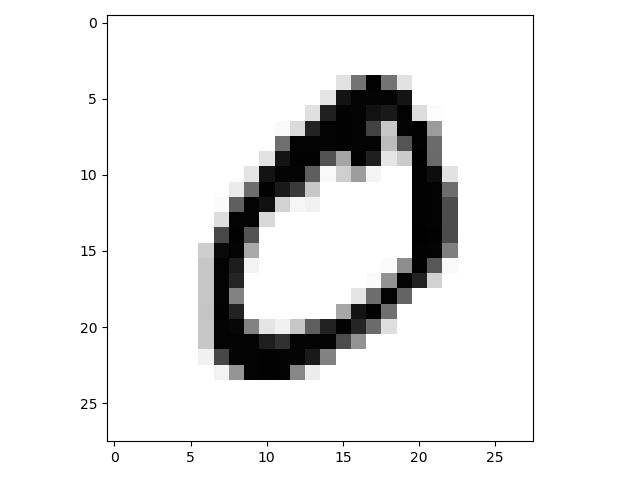
\includegraphics[width=0.1\textwidth]{figure/0.png}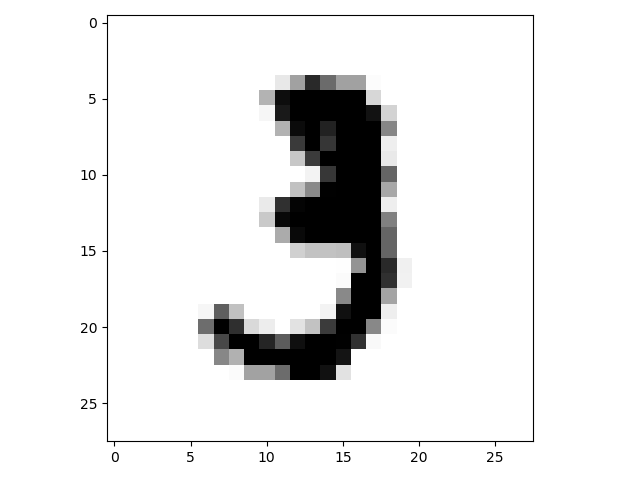
\includegraphics[width=0.1\textwidth]{figure/3.png}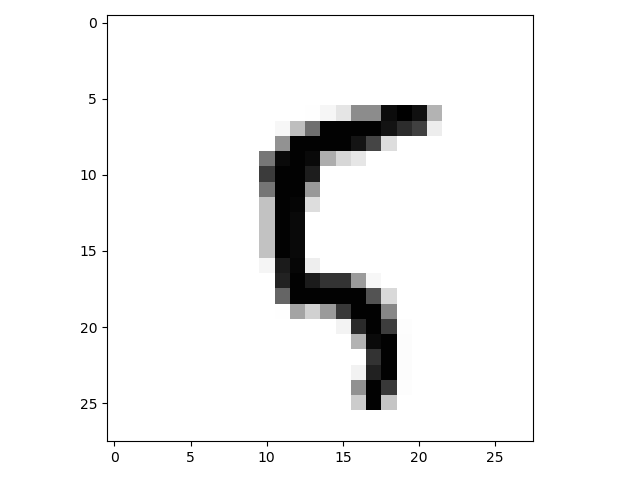
\includegraphics[width=0.1\textwidth]{figure/5.png}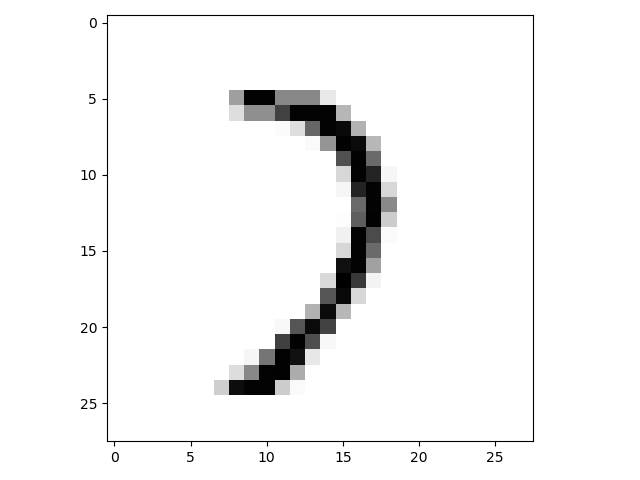
\includegraphics[width=0.1\textwidth]{figure/2.png}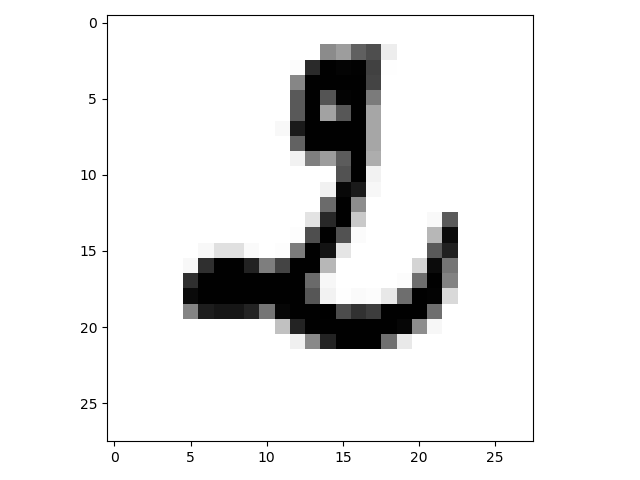
\includegraphics[width=0.1\textwidth]{figure/8.png}}
\caption{Example of data}
\label{Example of data}
\end{figure}
\end{frame}



\subsection{Data transformation}
\begin{frame}{\secname : \subsecname}
	\begin{itemize}
  \item Besides, the data can't be normalized since there are some constant valued columns (some columns are always $0$). 
  \item Alternatively, We will map these values into an interval from $[0.01, 1]$ by multiplying each pixel that values $p$ with \eqref{pnew}.
\begin{equation}
	p^{new}=p*\frac{0.99}{255}+0.01\label{pnew}
\end{equation}
	\begin{itemize}
	  \item It will speed the computation if we map the data to $[0.01, 1]$, rather than $[0, 1]$.
	\end{itemize}

\end{itemize}

\end{frame}




\section{Data visualization}
\begin{frame}[allowframebreaks]{\secname}
\begin{figure}[htbp]
\centerline{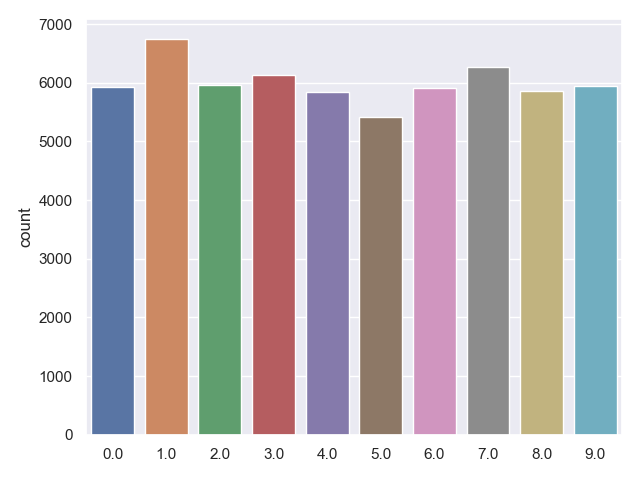
\includegraphics[width=0.6\textwidth]{figure/distributionplot.png}}
\caption{Distribution of MNIST data}
\label{Distribution of MNIST data}
\end{figure}
\begin{itemize}
  \item From Fig. \ref{Distribution of MNIST data}, we can conclude that the data size of different class are basically equal, which means that our data is balanced.
\end{itemize}
\end{frame}



%\section{Variable Selection} 







\section{Used Language}
\begin{frame}[allowframebreaks]{\secname}
	\begin{itemize}
  \item We are originally use R language as our tool to model \begin{itemize}
  \item by the limited computing ability, we only randomly pick 6,000 train and 1,000 test data from all numerate data from (0-9) to train our model, which is $1/10$ of the MNIST data set. 
  \item However, even if we reduced the data size, we still find the running time is extremely long when tuning model of Neural Network in \ref{nn}. 
\end{itemize}

  \item Since Python is up to 8 times faster than R. Therefore, we only use R as our visualization programming language and Python as our model building language.
\end{itemize}

\end{frame}




\section{Support Vector Machines}
\begin{frame}[allowframebreaks]{\secname}
	\begin{itemize}
  \item In machine learning, support-vector machines (SVMs, also support-vector networks[1]) are supervised learning models with associated learning algorithms that analyze data used for classification and regression analysis.
  \item Since it's time consuming to use quadratic programing in SVM, so we adapted Stochastic Sub-Gradient Descent into Linear Kernel SVM.
\end{itemize}

%If n\_class is the number of classes, then $n_class * (n_class - 1) / 2$ classifiers are constructed and each one trains data from two classes. 
\end{frame}



\subsection{Linear Kernel}
\subsubsection{SGD optimization}\label{svmlkgo}
\begin{frame}[allowframebreaks]{\secname : \subsecname}{\subsubsecname}
First we use support vector machines of linear kernel. 
$$
K\left\langle x, x^{\prime}\right\rangle=\left\langle x, x^{\prime}\right\rangle
$$	
We added Elastic-Net regularization term (See \eqref{elas} for the math formula of Elastic-Net) into our SVM model which linearly combines the L1 and L2 penalties of the lasso and ridge methods, and included two parameters:
\begin{itemize}
  \item $l_{1_{ratio}}$: weight of $L_1$ regularization term;
  \item $\alpha$: overall penalization term.
\end{itemize}
\begin{equation}\label{elas}
	R(w) := \alpha(\frac{1-l_{1_{ratio}}}{2} \sum_{i=1}^{n} w_i^2 + l_{1_{ratio}} \sum_{i=1}^{n} |w_i|)
\end{equation}

Applying this regularization term into SVM model, and tuning these 2 parameters, the results are as Fig. \ref{SGD SVM Accuracy rate, alpha versus l1 ratio}. 

\framebreak
From figure, we can easily see that a smaller $\alpha$ tend to be better, which means that there is barely improvement on test error by using regularization term. Therefore, we don't consider regularization term in the following SVM models.  
\begin{figure}[htbp]
\centerline{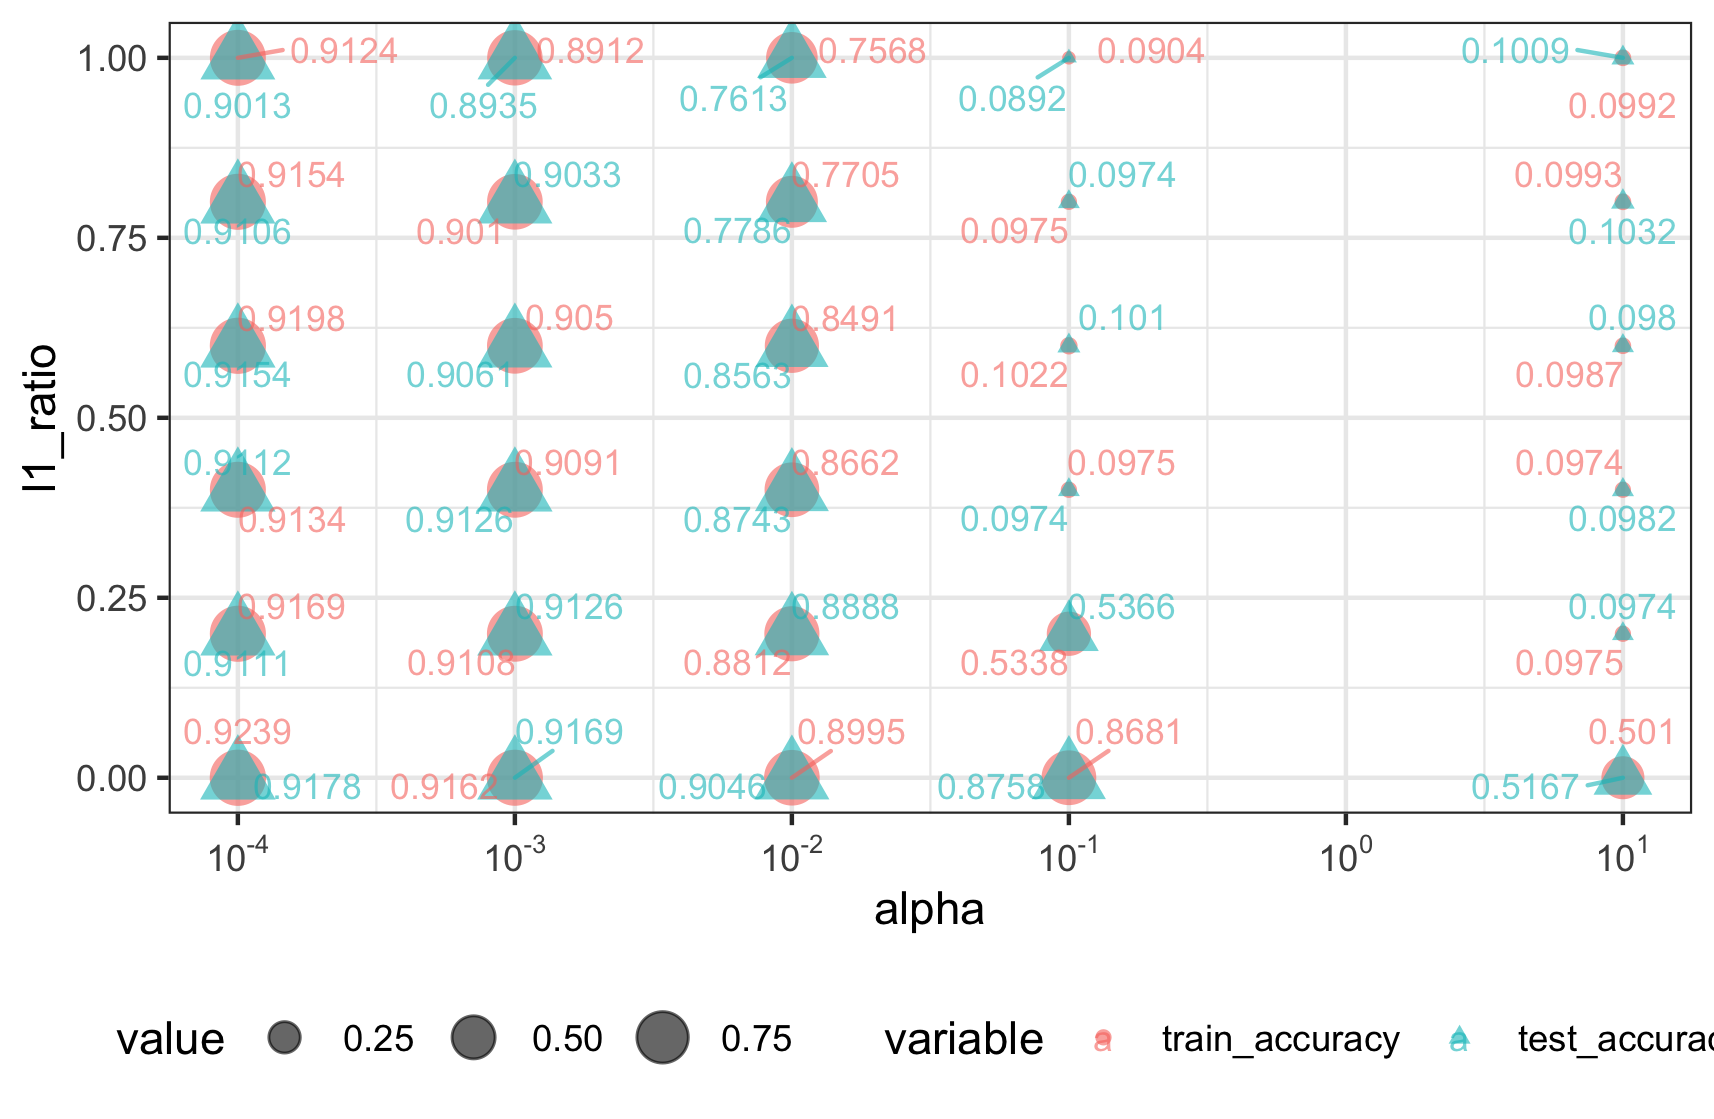
\includegraphics[width=0.8\textwidth]{figure/SGD SVM Accuracy rate, alpha versus l1_ratio.png}}
\caption{SGD SVM Accuracy rate, alpha versus l1 ratio}
\label{SGD SVM Accuracy rate, alpha versus l1 ratio}
\end{figure}


We pick the model of best test accuracy, which is 0.9178, and the confusion table is as TABLE \ref{SVM confusion table}.
%\begin{figure}[htbp]
%\centerline{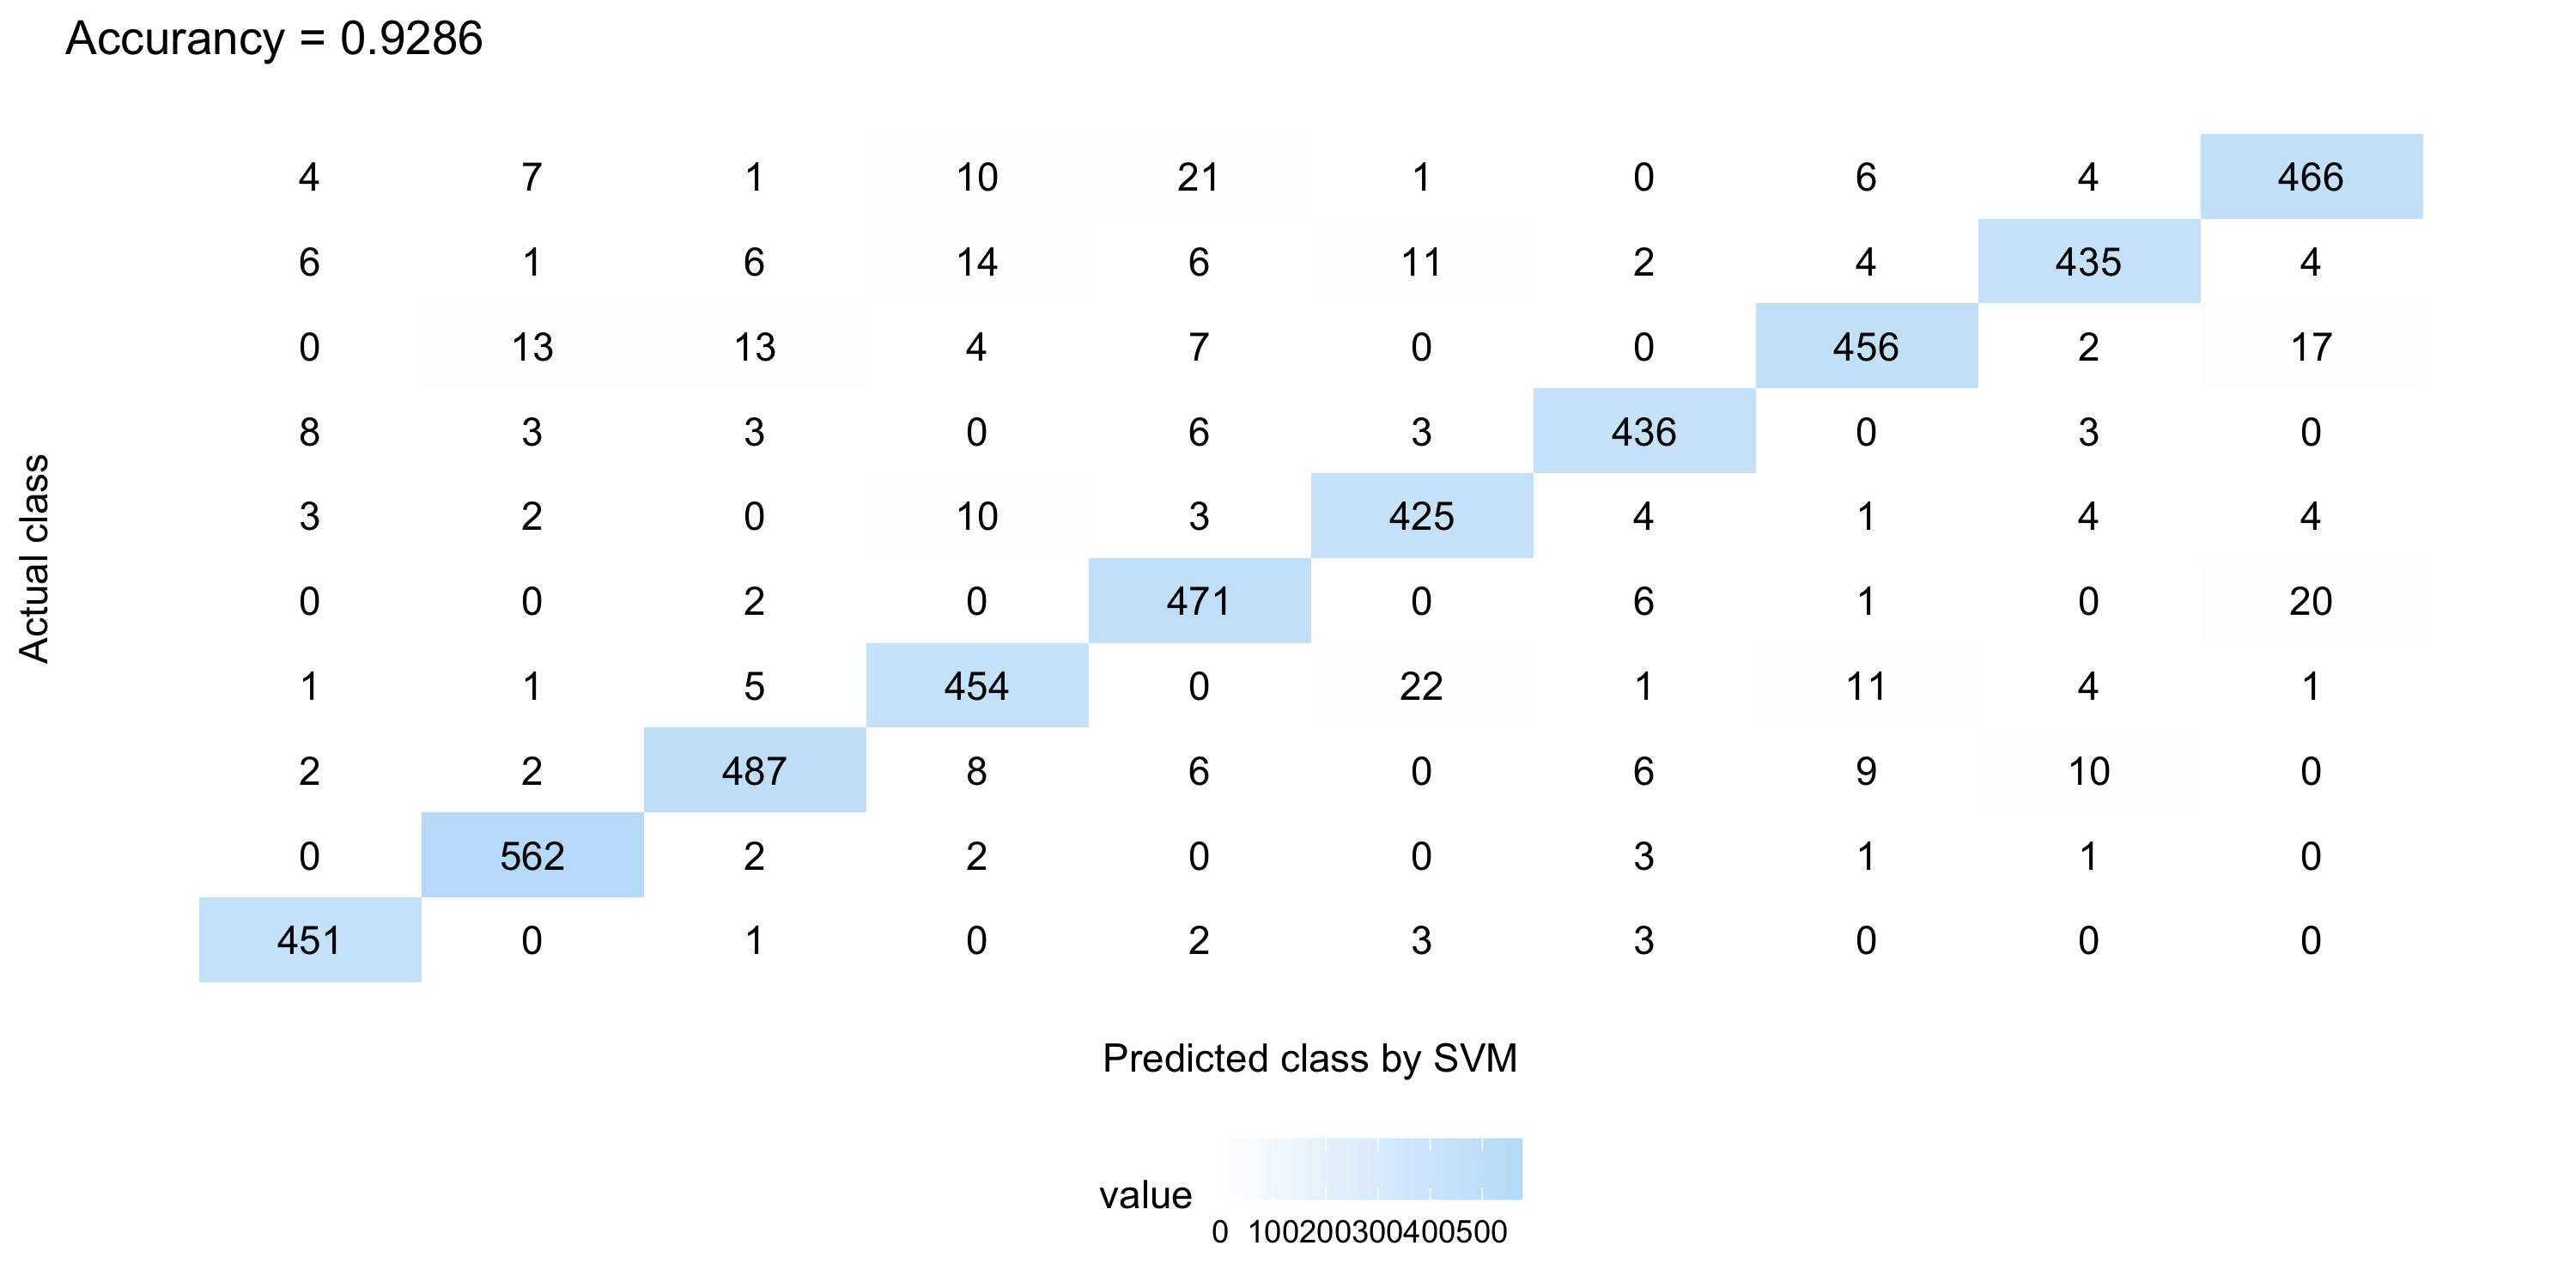
\includegraphics[width=0.8\textwidth]{figure/errorSVM.png}}
%\caption{Predicted class vs Actual class}
%\label{errorSVM}
%\end{figure}
% Table generated by Excel2LaTeX from sheet 'Sheet1'

\begin{table}[htbp]
\tiny
  \centering
  \caption{SVM confusion table}
% Table generated by Excel2LaTeX from sheet 'Sheet2'
\begin{tabular}{|r|rrrrrrrrrr|r|}
\hline
  & 0 & 1 & 2 & 3 & 4 & 5 & 6 & 7 & 8 & 9 &  \\
\hline
0 & 953 & 0 & 1 & 2 & 0 & 16 & 3 & 4 & 1 & 0 & 0.9724 \\
1 & 0 & 1106 & 3 & 1 & 1 & 5 & 4 & 2 & 13 & 0 & 0.9744 \\
2 & 7 & 3 & 899 & 19 & 9 & 20 & 15 & 17 & 39 & 4 & 0.8711 \\
3 & 6 & 0 & 16 & 899 & 2 & 50 & 4 & 11 & 13 & 9 & 0.8901 \\
4 & 1 & 1 & 7 & 0 & 926 & 0 & 7 & 4 & 4 & 32 & 0.9430 \\
5 & 6 & 1 & 0 & 22 & 12 & 814 & 14 & 4 & 14 & 5 & 0.9126 \\
6 & 11 & 3 & 3 & 2 & 5 & 30 & 901 & 1 & 2 & 0 & 0.9405 \\
7 & 1 & 5 & 19 & 4 & 4 & 4 & 1 & 969 & 2 & 19 & 0.9426 \\
8 & 9 & 7 & 4 & 24 & 24 & 83 & 11 & 18 & 784 & 10 & 0.8049 \\
9 & 8 & 4 & 0 & 10 & 47 & 22 & 1 & 38 & 9 & 870 & 0.8622 \\
\hline
  & 0.9511 & 0.9788 & 0.9443 & 0.9145 & 0.8990 & 0.7797 & 0.9376 & 0.9073 & 0.8899 & 0.9168 & 0.9178 \\
\hline
\end{tabular}%
  \label{SVM confusion table}%
\end{table}%
\end{frame}





\subsection{RBF Kernel}
\subsubsection{Tuning with 20\% data set}
\begin{frame}[allowframebreaks]{\secname : \subsecname}{\subsubsecname}
In order to get a non-linear boundary, we use RBF kernel to train model.
$$
K\left\langle x, x^{\prime}\right\rangle=\exp \left(-\gamma\left\|x-x^{\prime}\right\|^{2}\right) 
$$

Considering the computation complexity of RBF Kernel, we only use 20\% data set to tune our model. The hyper-parameter field are as follows.
\begin{itemize}
  \item $\gamma:10^{-4},10^{-3},10^{-2},10^{-1}$.
\end{itemize}

\framebreak
It takes total 13,578.077 seconds to train those 4 model with 4-core CPU. And we gain best model of $\gamma=0.01$ with a test accuracy of $0.9375$, training this model takes 2,749.068 seconds.
\begin{figure}[htbp]
\centerline{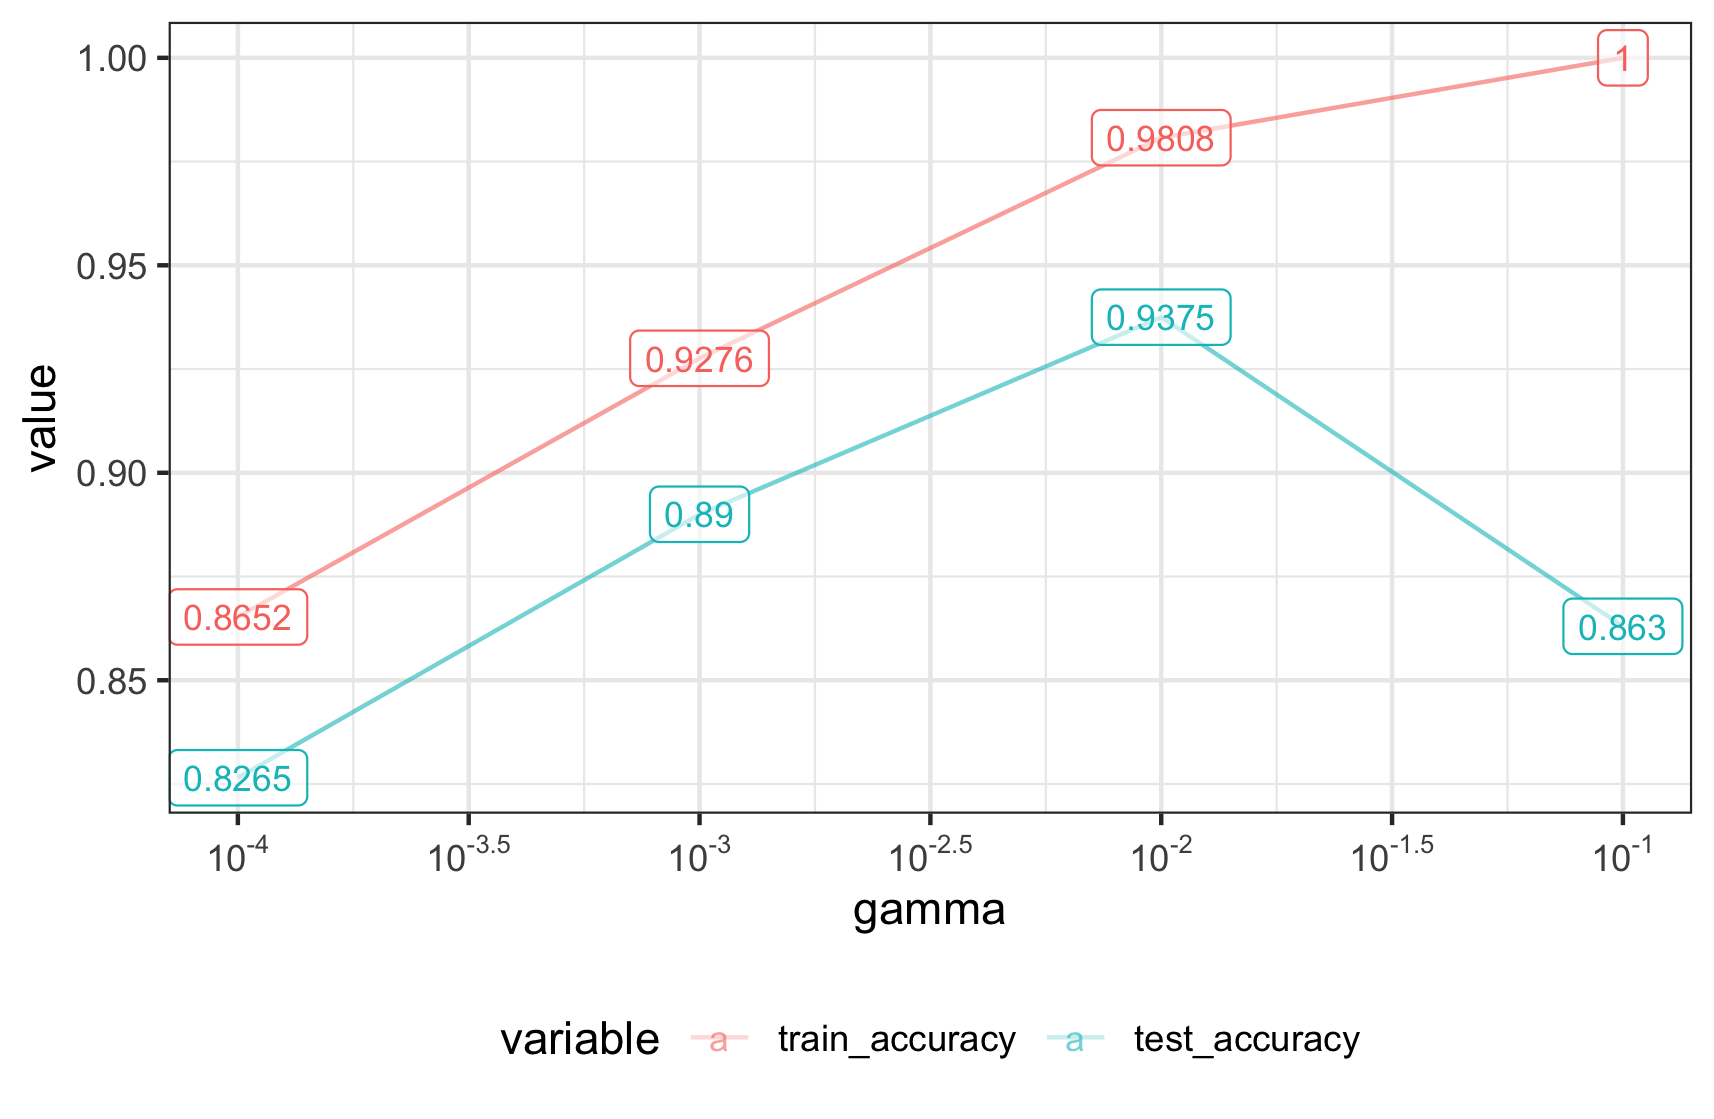
\includegraphics[width=0.8\textwidth]{figure/RBF SVM Accuracy versus gamma.png}}
\caption{RBF SVM Accuracy versus gamma}
\label{RBF SVM Accuracy versus gamma}
\vspace{-1.5em}
\end{figure}
\end{frame}









\subsubsection{Train best model with whole data set}
\begin{frame}[allowframebreaks]{\secname : \subsecname}{\subsubsecname}
Applying best model of $\gamma=0.01$ to whole data set. It takes total 2,749 seconds to train this model with 4-core CPU. We get a train accuracy of 0.9983 and test accuracy of $0.9852$, and the confusion table is as TABLE \ref{tab:RBF SVM confusion table}.
% Table generated by Excel2LaTeX from sheet 'Sheet1'
\begin{table}[htbp]
\tiny
  \centering
  \caption{RBF SVM confusion table}
% Table generated by Excel2LaTeX from sheet 'Sheet2'
\begin{tabular}{|r|rrrrrrrrrr|r|}
\hline
  & 0 & 1 & 2 & 3 & 4 & 5 & 6 & 7 & 8 & 9 &  \\
\hline
0 & 1014 & 0 & 2 & 0 & 0 & 2 & 2 & 0 & 1 & 3 & 0.9902 \\
1 & 0 & 1177 & 2 & 1 & 1 & 0 & 1 & 0 & 2 & 1 & 0.9932 \\
2 & 2 & 2 & 1037 & 2 & 0 & 0 & 0 & 2 & 5 & 1 & 0.9867 \\
3 & 0 & 0 & 3 & 1035 & 0 & 5 & 0 & 6 & 6 & 2 & 0.9792 \\
4 & 0 & 0 & 1 & 0 & 957 & 0 & 1 & 2 & 0 & 3 & 0.9927 \\
5 & 1 & 1 & 0 & 4 & 1 & 947 & 4 & 0 & 5 & 1 & 0.9824 \\
6 & 2 & 0 & 1 & 0 & 2 & 0 & 1076 & 0 & 4 & 0 & 0.9917 \\
7 & 1 & 1 & 8 & 1 & 1 & 0 & 0 & 1110 & 2 & 4 & 0.9840 \\
8 & 0 & 4 & 2 & 4 & 1 & 6 & 0 & 1 & 1018 & 1 & 0.9817 \\
9 & 3 & 1 & 0 & 7 & 5 & 2 & 0 & 4 & 9 & 974 & 0.9692 \\
\hline
  & 0.9912 & 0.9924 & 0.9820 & 0.9820 & 0.9886 & 0.9844 & 0.9926 & 0.9867 & 0.9677 & 0.9838 & 0.9852 \\
\hline
\end{tabular}%
  \label{tab:RBF SVM confusion table}%
\end{table}%	
\end{frame}









\subsection{Polynomial Kernel}
\subsubsection{Tuning with 20\% data set}
\begin{frame}[allowframebreaks]{\secname : \subsecname}{\subsubsecname}
We now use Polynomial kernel to train model.
$$
K\left\langle x, x^{\prime}\right\rangle=\left(\gamma\left\langle x, x^{\prime}\right\rangle\right)^{d}
$$	
\begin{itemize}
  \item Considering the computation complexity of Polynomial Kernel, we only use 20\% data set to tune our model. 
  \item The hyper-parameter field are as follows.
	\begin{itemize}
	  \item $\gamma:10^{-4},10^{-3},10^{-2},10^{-1}$;
	  \item $d=1,2,3,4,5$.
	\end{itemize}
\end{itemize}


\framebreak
It takes total 4,916.98 seconds to tune the model with 4-core CPU. And we gain best model of $\gamma=0.1,d=2$. We get a test accuracy of $0.9535$.
\begin{figure}[htbp]
\centerline{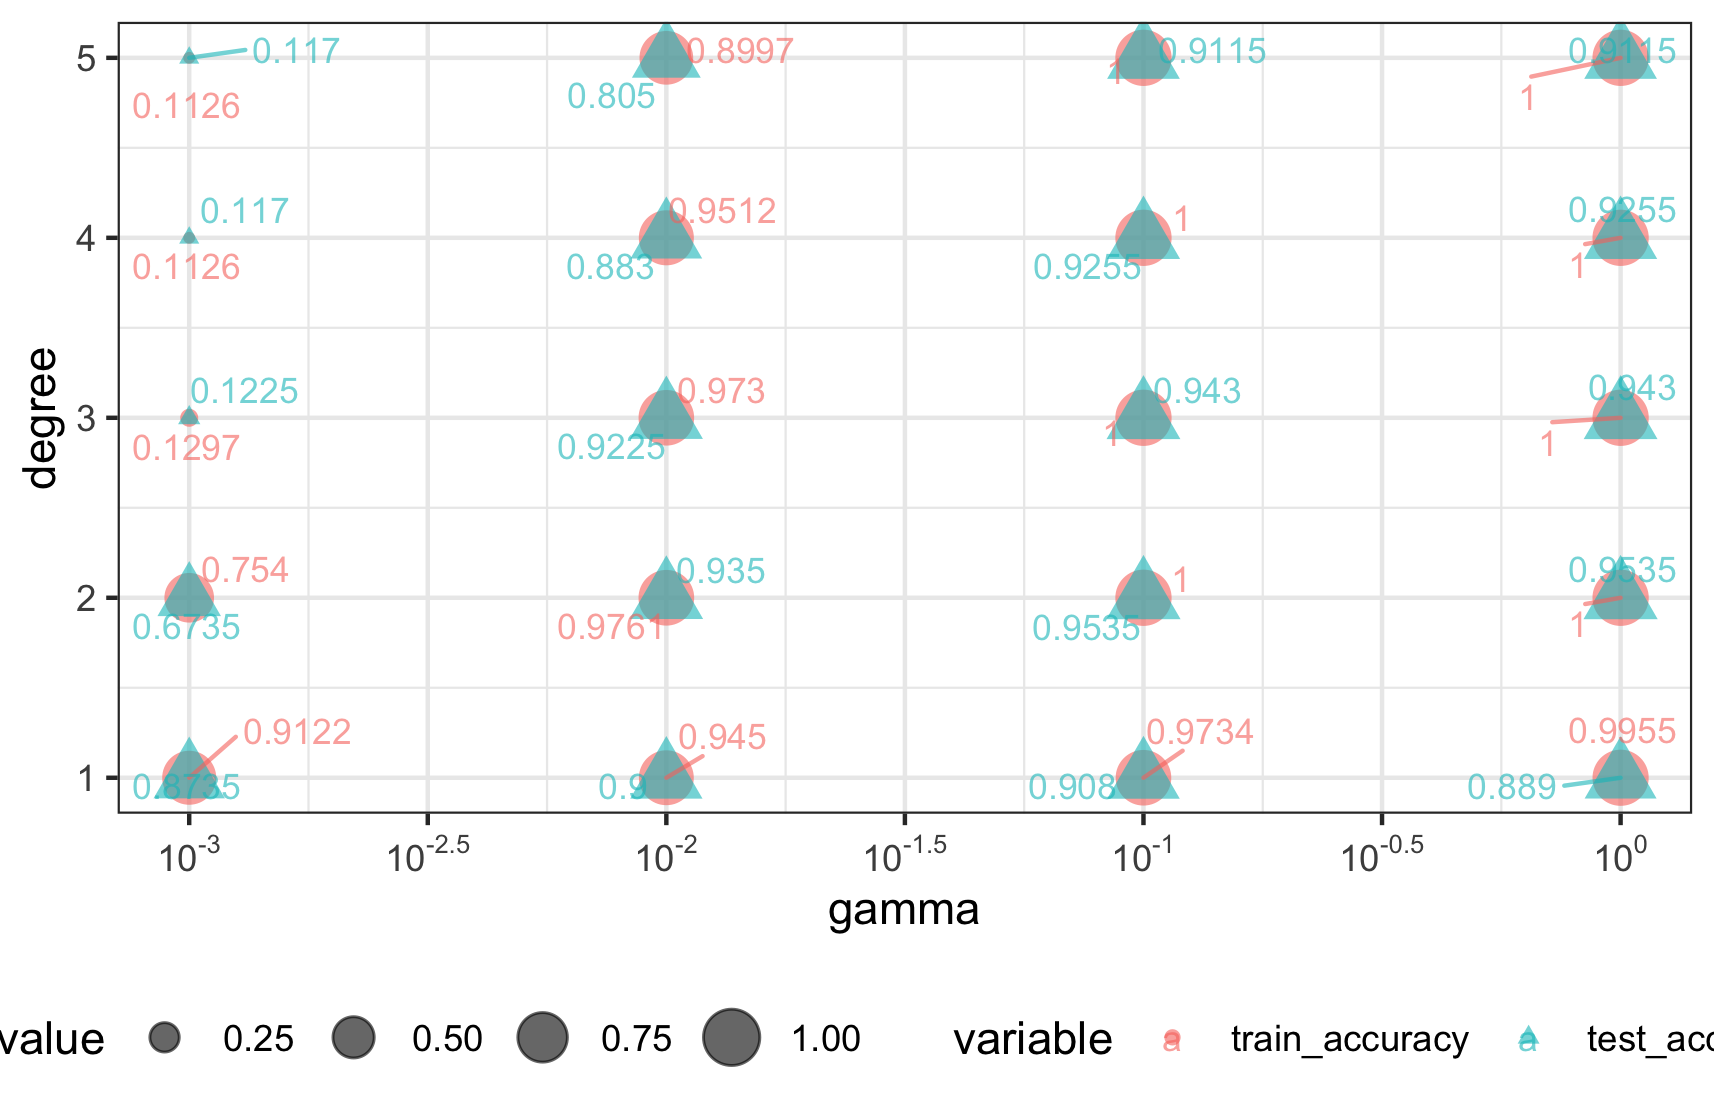
\includegraphics[width=0.8\textwidth]{figure/Polynomial SVM Accuracy degree versus gamma.png}}
\caption{Polynomial SVM Accuracy degree versus gamma}
\label{Polynomial SVM Accuracy degree versus gamma}
\vspace{-1.5em}
\end{figure}
\end{frame}

\subsubsection{Train best model with whole data set}
\begin{frame}[allowframebreaks]{\secname : \subsecname}{\subsubsecname}
Applying best model of $\gamma=0.1,d=2$ to whole data set. It takes total 1,439.43 seconds to train this model with 4-core CPU. We get a train accuracy of $0.9989$ and a test accuracy of $0.9806$, and the confusion table is as TABLE \ref{tab:Polynomial SVM confusion table}.
% Table generated by Excel2LaTeX from sheet 'Sheet1'
\begin{table}[htbp]
\tiny
  \centering
  \caption{Polynomial SVM confusion table}
% Table generated by Excel2LaTeX from sheet 'Sheet2'
\begin{tabular}{|r|rrrrrrrrrr|r|}
\hline
  & 0 & 1 & 2 & 3 & 4 & 5 & 6 & 7 & 8 & 9 &  \\
\hline
0 & 973 & 0 & 1 & 2 & 0 & 1 & 1 & 0 & 2 & 0 & 0.9929 \\
1 & 0 & 1128 & 2 & 1 & 0 & 1 & 1 & 1 & 1 & 0 & 0.9938 \\
2 & 7 & 1 & 1008 & 1 & 1 & 0 & 4 & 6 & 4 & 0 & 0.9767 \\
3 & 0 & 0 & 3 & 987 & 0 & 5 & 0 & 5 & 7 & 3 & 0.9772 \\
4 & 1 & 0 & 4 & 0 & 966 & 0 & 2 & 0 & 0 & 9 & 0.9837 \\
5 & 2 & 0 & 0 & 9 & 1 & 872 & 3 & 1 & 2 & 2 & 0.9776 \\
6 & 5 & 2 & 2 & 0 & 2 & 5 & 940 & 0 & 2 & 0 & 0.9812 \\
7 & 0 & 6 & 9 & 1 & 1 & 0 & 0 & 1002 & 1 & 8 & 0.9747 \\
8 & 4 & 0 & 2 & 4 & 3 & 2 & 1 & 4 & 951 & 3 & 0.9764 \\
9 & 2 & 4 & 0 & 4 & 9 & 4 & 0 & 4 & 3 & 979 & 0.9703 \\
\hline
  & 0.9789 & 0.9886 & 0.9777 & 0.9782 & 0.9827 & 0.9798 & 0.9874 & 0.9795 & 0.9774 & 0.9751 & 0.9806 \\
\hline
\end{tabular}%
  \label{tab:Polynomial SVM confusion table}%
\end{table}%	
\end{frame}















\section{Boosting}
\subsection{Ada Boosting}
\subsubsection{Tuning with 20\% data set}
\begin{frame}[allowframebreaks]{\secname : \subsecname}{\subsubsecname}
It takes total 1,044 seconds to tune the model with 4-core CPU. And we gain best model of learning rate $=0.1$.	
\begin{figure}[htbp]
\centerline{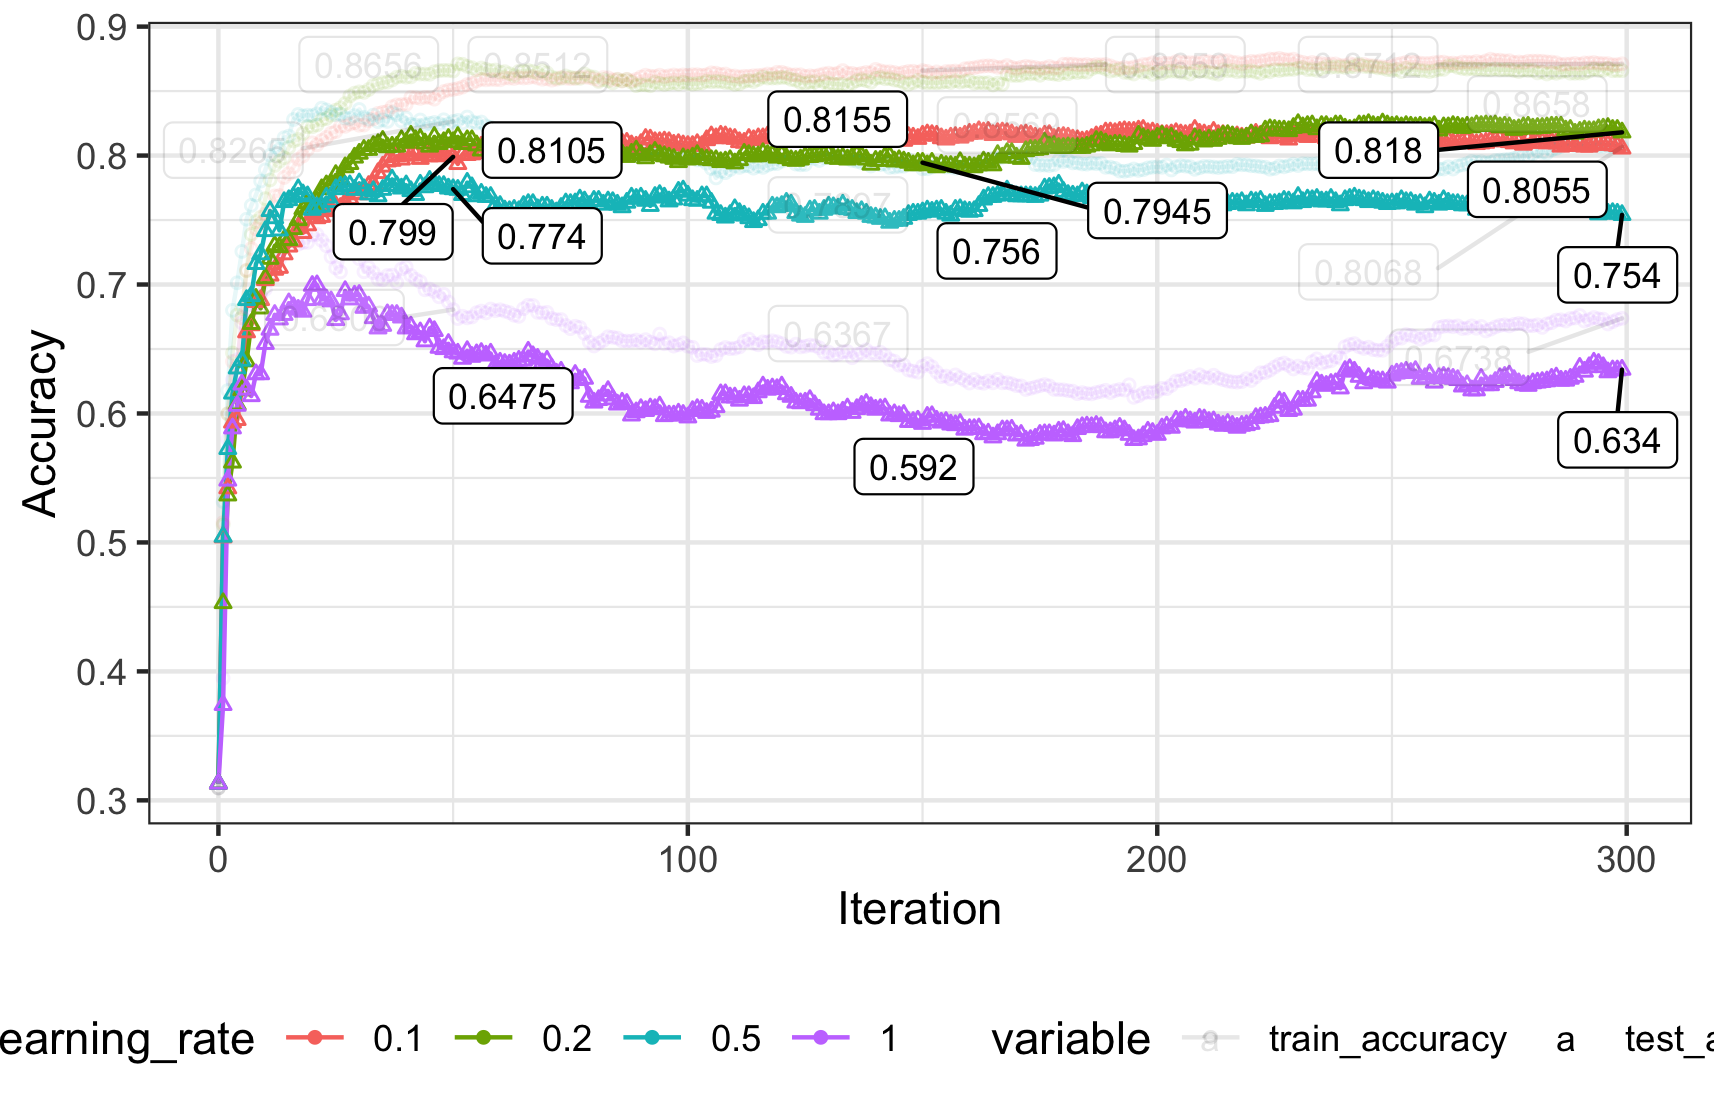
\includegraphics[width=0.8\textwidth]{figure/Ada Boosting Accuracy By Iteration.png}}
\caption{Ada Boosting Accuracy By Iteration}
\label{Ada Boosting Accuracy By Iteration}
\vspace{-1.5em}
\end{figure}
\end{frame}



\subsubsection{Train best model with whole data set}
\begin{frame}[allowframebreaks]{\secname : \subsecname}{\subsubsecname}
\begin{itemize}
  \item Now we apply the best model of learning rate $=0.1$ into whole data
  \item it takes 1402 seconds to  train the model
  \item The test accuracy is 0.8902, train accuracy is 0.8911, and the confusion table is as TABLE \ref{tab:Ada Boosting confusion table}. 
  \item However from Fig. \ref{Final Ada Boosting Accuracy By Iteration}, we can see that there are barely differences between the test and train accuracy in each iteration, which means that our model is under-fitted. Try to increase the iteration number and decrease the learning rate might increase accuracy.
\end{itemize}


\begin{figure}[htbp]
\centerline{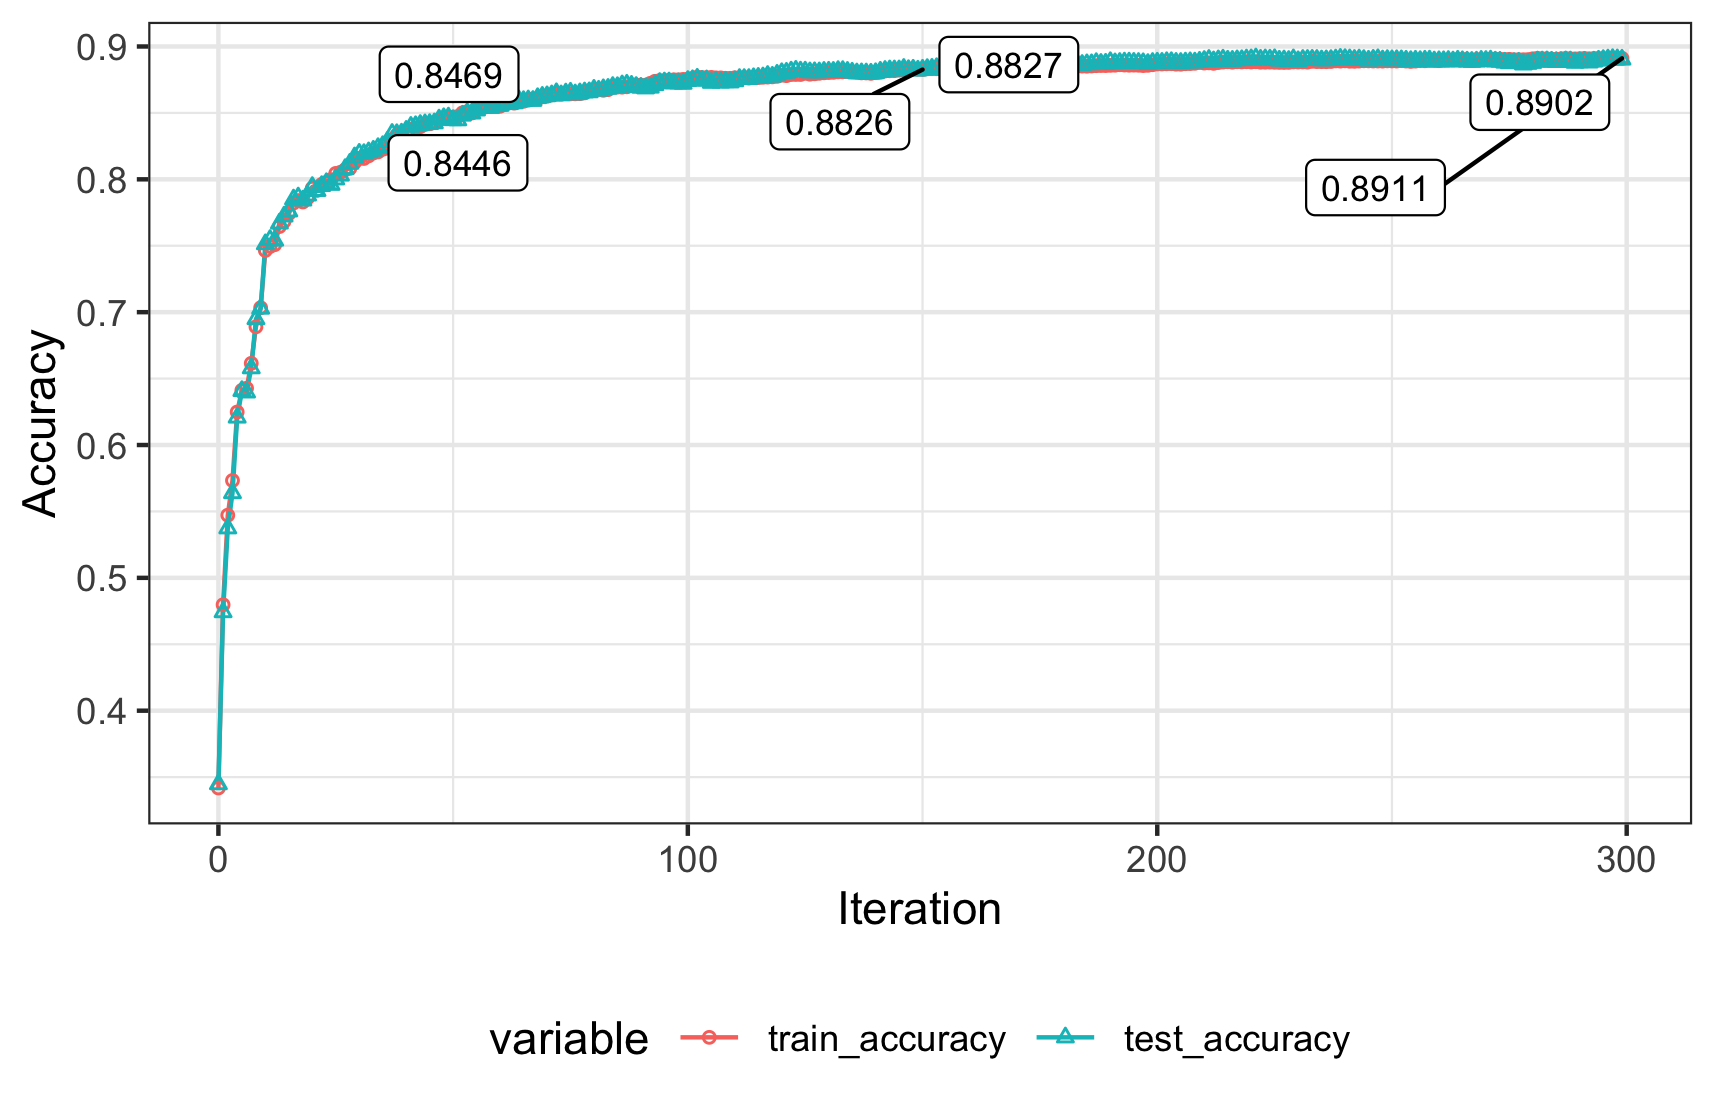
\includegraphics[width=0.8\textwidth]{figure/Final Ada Boosting Accuracy By Iteration.png}}
\caption{Final Ada Boosting Accuracy By Iteration}
\label{Final Ada Boosting Accuracy By Iteration}
\end{figure}
% Table generated by Excel2LaTeX from sheet 'Sheet1'
\begin{table}[htbp]
\tiny
  \centering
  \caption{Ada Boosting confusion table}
\begin{tabular}{|r|rrrrrrrrrr|r|}
\hline
  & 0 & 1 & 2 & 3 & 4 & 5 & 6 & 7 & 8 & 9 &  \\
\hline
0 & 902 & 0 & 13 & 0 & 0 & 45 & 13 & 0 & 4 & 3 & 0.9204 \\
1 & 0 & 1114 & 5 & 3 & 0 & 1 & 1 & 1 & 8 & 2 & 0.9815 \\
2 & 12 & 14 & 852 & 16 & 8 & 5 & 38 & 9 & 76 & 2 & 0.8256 \\
3 & 20 & 0 & 13 & 894 & 0 & 30 & 0 & 7 & 43 & 3 & 0.8851 \\
4 & 1 & 0 & 6 & 0 & 902 & 1 & 2 & 1 & 8 & 61 & 0.9185 \\
5 & 16 & 3 & 3 & 46 & 3 & 754 & 13 & 1 & 38 & 15 & 0.8453 \\
6 & 10 & 3 & 44 & 0 & 31 & 29 & 833 & 0 & 8 & 0 & 0.8695 \\
7 & 0 & 3 & 27 & 4 & 6 & 0 & 0 & 889 & 8 & 91 & 0.8648 \\
8 & 12 & 10 & 3 & 18 & 8 & 11 & 4 & 3 & 891 & 14 & 0.9148 \\
9 & 4 & 8 & 7 & 12 & 56 & 2 & 0 & 12 & 24 & 884 & 0.8761 \\
\hline
% Table generated by Excel2LaTeX from sheet 'Sheet2'
  & 0.9232 & 0.9645 & 0.8756 & 0.9003 & 0.8895 & 0.8588 & 0.9215 & 0.9632 & 0.8042 & 0.8223 & 0.8911 \\
\hline
\end{tabular}%
 \label{tab:Ada Boosting confusion table}%
\end{table}%	
\end{frame}



\subsection{Gradient Boosting}
\subsubsection{Tuning with 20\% data set}
\begin{frame}[allowframebreaks]{\secname : \subsecname}{\subsubsecname}
\begin{itemize}
  \item Even though we only training model with 20\% data, Gradient Boosting still need an average of 15 minutes to build one model, which is significantly slower than ada boosting method. 
  \item It takes 12,129 seconds to tune parameters. 
\end{itemize}

\framebreak
From Fig. \ref{Gradient Boosting Accuracy By Iteration}, we can see that with the increasing of tree depth, the accuracies are going up. The best hyper parameters are learning rate $=0.2,$ tree depth $=4$. \footnote{Since the size of tree depth we choose is the upper bound of our tuning field, therefore, we might gain a better result by using a tree depth that is more than 4.}
\begin{figure}[htbp]
\centerline{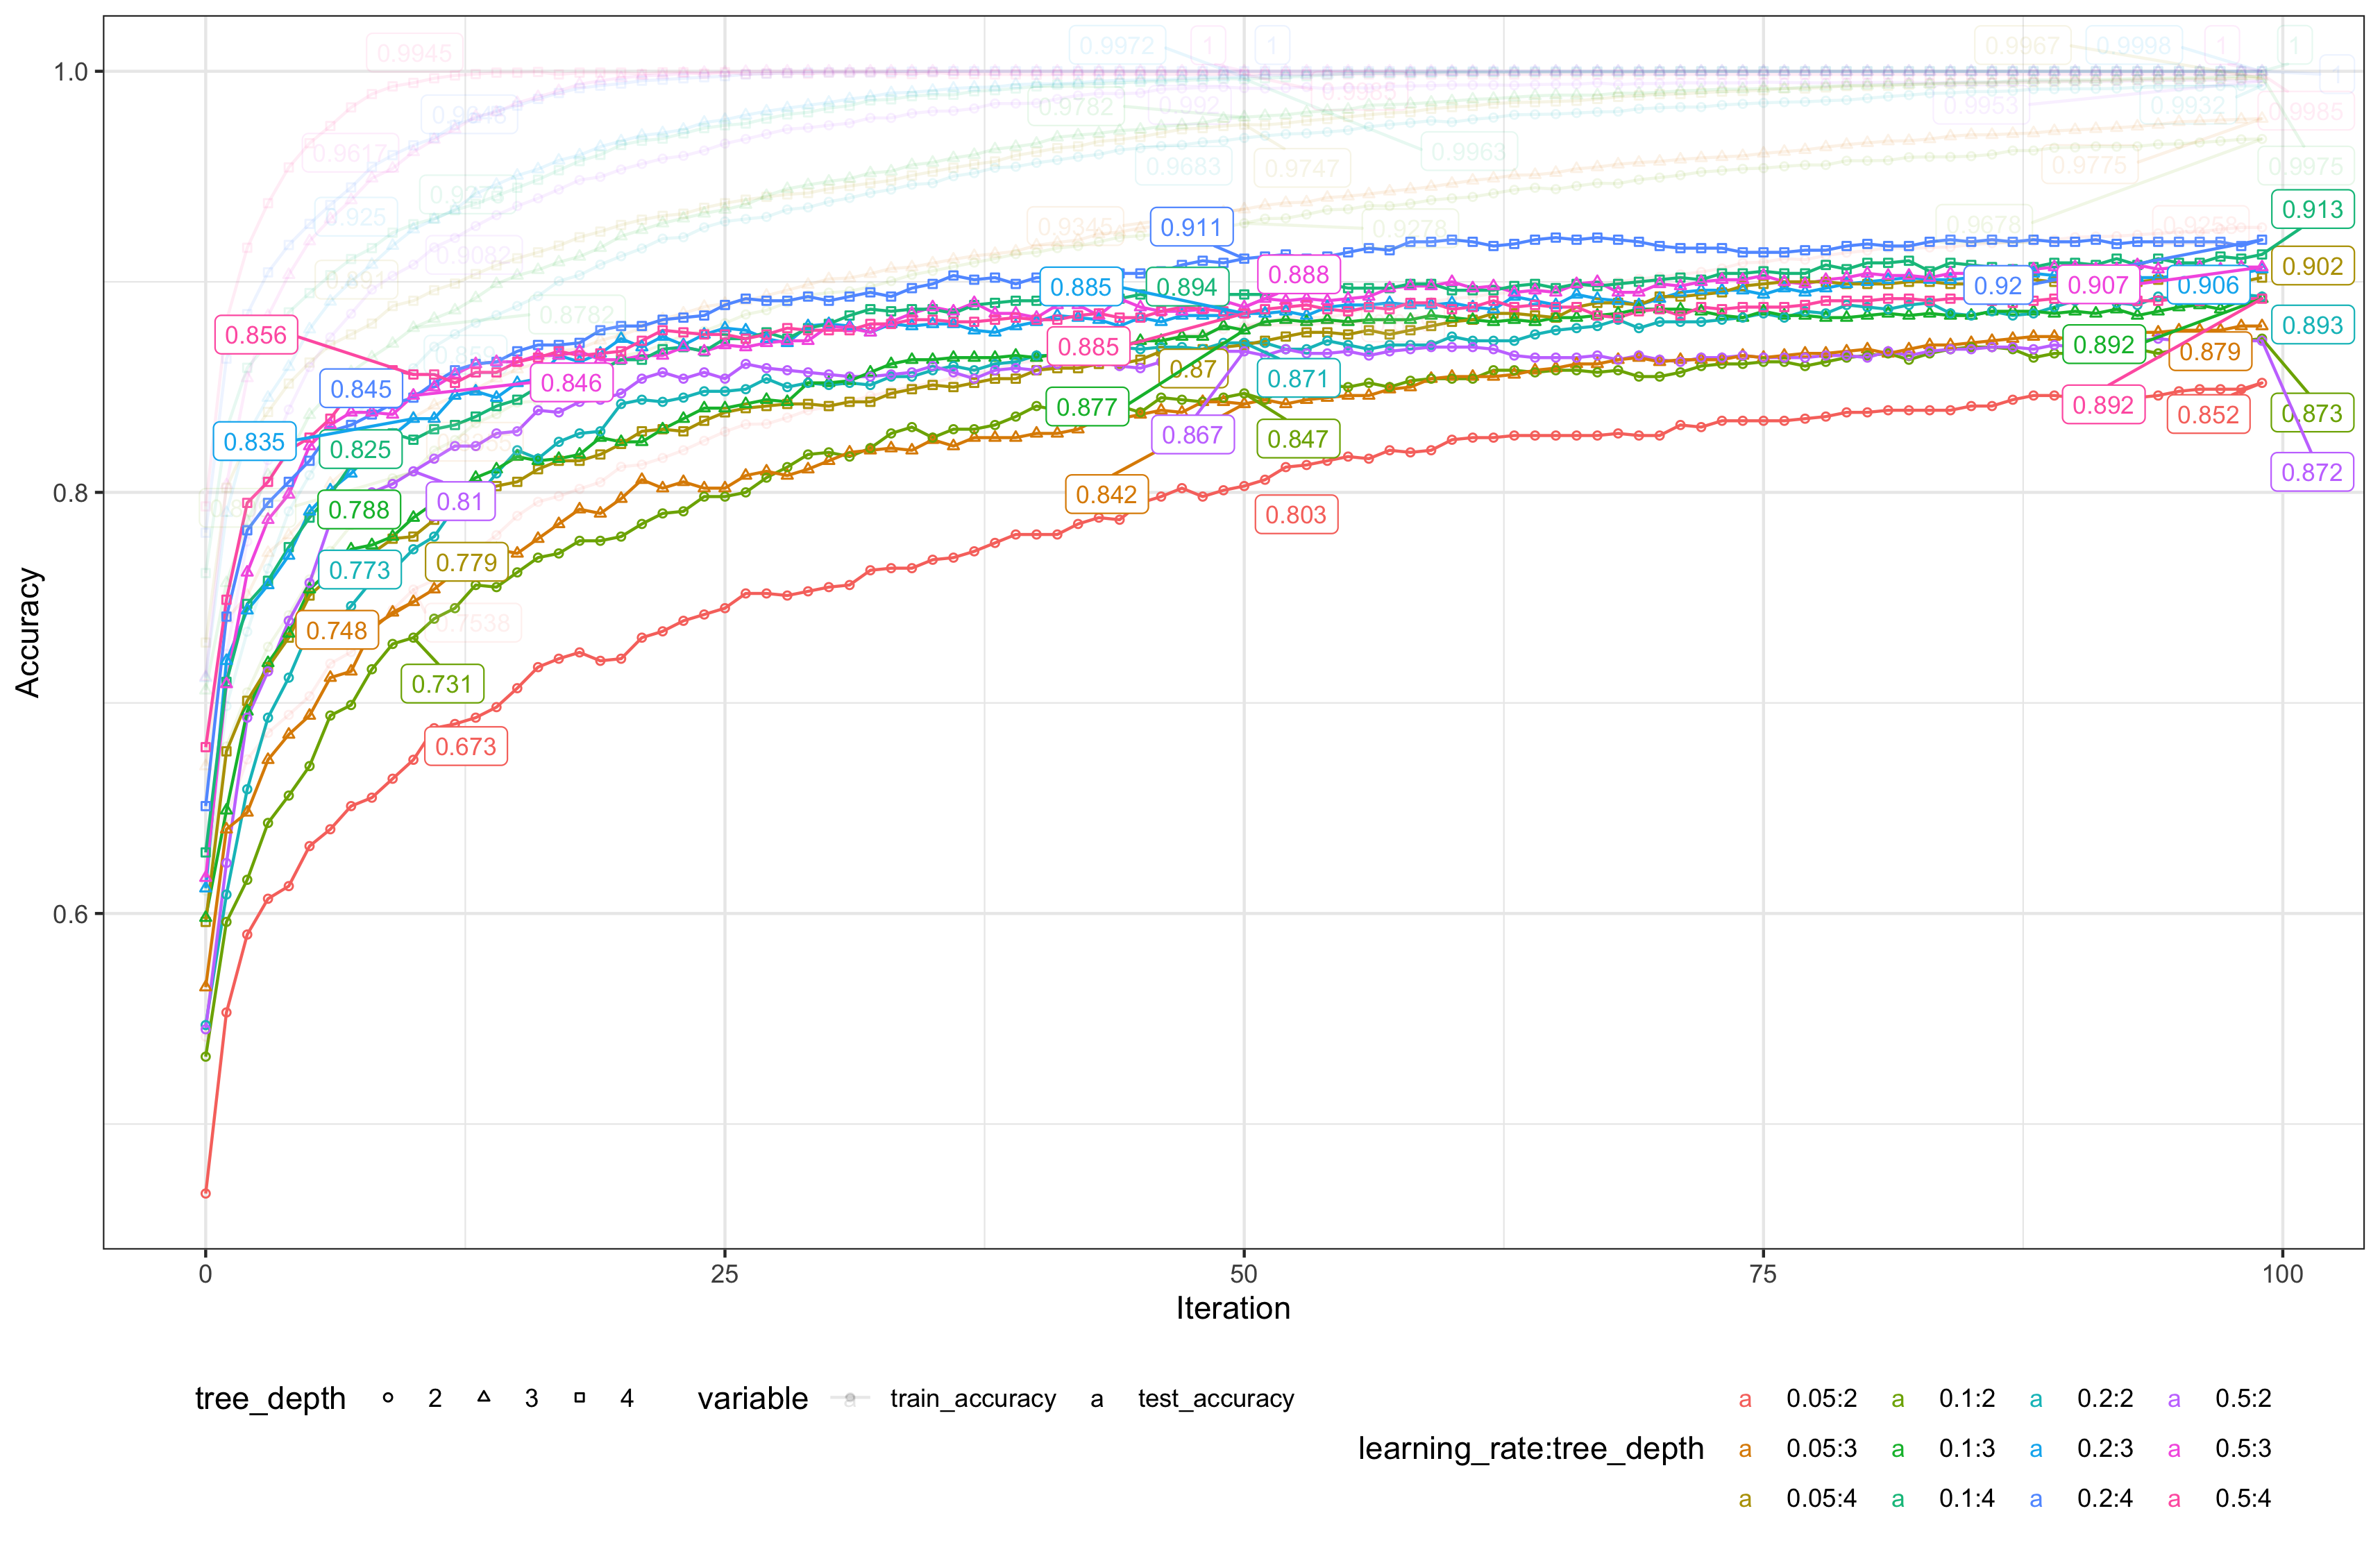
\includegraphics[width=0.7\textwidth]{figure/Gradient Boosting Accuracy By Iteration.png}}
\caption{Gradient Boosting Accuracy By Iteration}
\label{Gradient Boosting Accuracy By Iteration}
\end{figure}	
\end{frame}



\subsubsection{Train best model with whole data set}
\begin{frame}[allowframebreaks]{\secname : \subsecname}{\subsubsecname}
Now we train the model of learning rate $=0.2,$ tree depth $=4$ with whole data set. It takes 7,321 seconds to train the model, the test accuracy is 0.9673, train accuracy is 0.9981, and the confusion table is as TABLE \ref{tab:Gradient Boosting confusion table}.


% Table generated by Excel2LaTeX from sheet 'Sheet1'
\begin{table}[htbp]
\tiny
  \centering
  \caption{Gradient Boosting confusion table}
\begin{tabular}{|r|rrrrrrrrrr|r|}
\hline
  & 0 & 1 & 2 & 3 & 4 & 5 & 6 & 7 & 8 & 9 &  \\
\hline
0 & 962 & 0 & 0 & 2 & 0 & 7 & 4 & 2 & 3 & 0 & 0.9816 \\
1 & 0 & 1121 & 2 & 1 & 1 & 1 & 4 & 1 & 4 & 0 & 0.9877 \\
2 & 5 & 2 & 995 & 7 & 3 & 2 & 1 & 8 & 8 & 1 & 0.9641 \\
3 & 1 & 1 & 6 & 960 & 1 & 18 & 0 & 8 & 9 & 6 & 0.9505 \\
4 & 1 & 0 & 1 & 0 & 960 & 1 & 5 & 0 & 3 & 11 & 0.9776 \\
5 & 2 & 1 & 0 & 1 & 2 & 871 & 5 & 1 & 6 & 3 & 0.9765 \\
6 & 7 & 3 & 1 & 0 & 4 & 14 & 922 & 1 & 6 & 0 & 0.9624 \\
7 & 1 & 7 & 10 & 5 & 3 & 1 & 0 & 985 & 1 & 15 & 0.9582 \\
8 & 2 & 1 & 3 & 4 & 5 & 7 & 2 & 6 & 940 & 4 & 0.9651 \\
9 & 3 & 7 & 1 & 7 & 10 & 8 & 1 & 7 & 8 & 957 & 0.9485 \\
\hline
% Table generated by Excel2LaTeX from sheet 'Sheet2'
  & 0.9776 & 0.9808 & 0.9764 & 0.9726 & 0.9707 & 0.9366 & 0.9767 & 0.9666 & 0.9514 & 0.9599 & 0.9673 \\
\hline
\end{tabular}%
 \label{tab:Gradient Boosting confusion table}%
\end{table}%	
\end{frame}



\section{Neutral Network}\label{nn}
\begin{frame}[allowframebreaks]{\secname}
A neural network is a series of algorithms that endeavors to recognize underlying relationships in a set of data through a process that mimics the way the human brain operates.
%\begin{figure}[htbp]
%\centerline{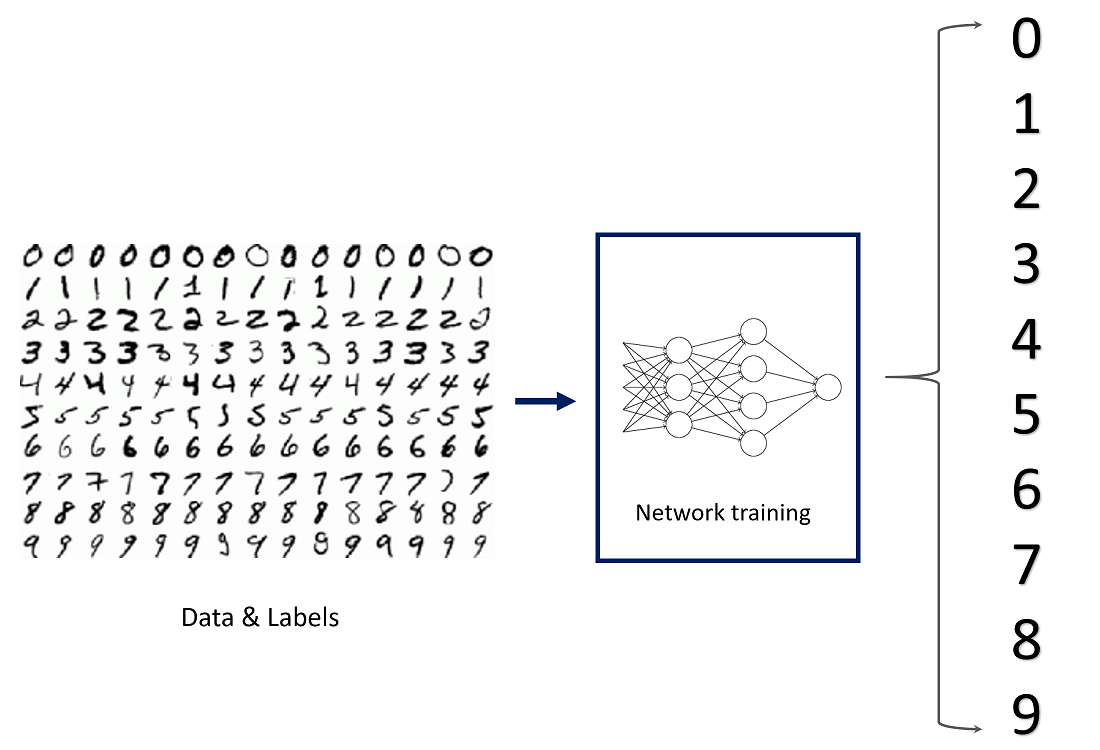
\includegraphics[width=0.2\textwidth]{figure/MNIST DATABASE}}
%\caption{Neural network}
%\label{neural network}
%\end{figure}
We use batch\footnote{Batch: a set of N samples. The samples in a batch are processed independently, in parallel. If training, a batch results in only one update to the model.
A batch generally approximates the distribution of the input data better than a single input.} and epoch\footnote{Epoch: an arbitrary cutoff, generally defined as "one pass over the entire dataset", used to separate training into distinct phases, which is useful for logging and periodic evaluation.} to update our parameters\cite{chollet2015keras}.
\end{frame}



\subsection{1-layer Neutral Network}
\subsubsection{Softmax activation function}\label{Softmax activation function}
\begin{frame}[allowframebreaks]{\secname : \subsecname}{\subsubsecname}
Softmax is a basic activation function because it not only maps our output to a [0,1] range but also maps each output in such a way that the total sum is 1.
$$
\sigma(\mathbf{z})_{j}=\frac{e^{\mathbf{z}_{j}}}{\sum_{k=1}^{K} e^{\mathbf{z}_{k}}} \quad \text { for } j=1, \ldots, K
$$

We trained 216 1-layer Neutral Network models with different hidden nodes, learning rates and bias, for every type of model we trained 10 epochs. The hyper-parameter field are as follows.
\begin{itemize}
  \item Bias: 1, None;
  \item Number of hidden nodes: 20, 50, 100, 150, 250, 500;
  \item batch size: 100, 200, 300;
  \item loss function: mean squared error, categorical cross entropy;
  \item Learning rate: 0.001, 0.01, 0.1.
\end{itemize}



\framebreak
Firstly, we need to know if all our model is converged. From Fig. \ref{1-layer Neural Network Test Accuracy By Epoch}, we get 9 models that are not converged. Therefore we need to add more epoch to those unconverged model until them converged, and then use the converged model's test accuracy as their final accuracy. 
\begin{figure}[htbp]
\centerline{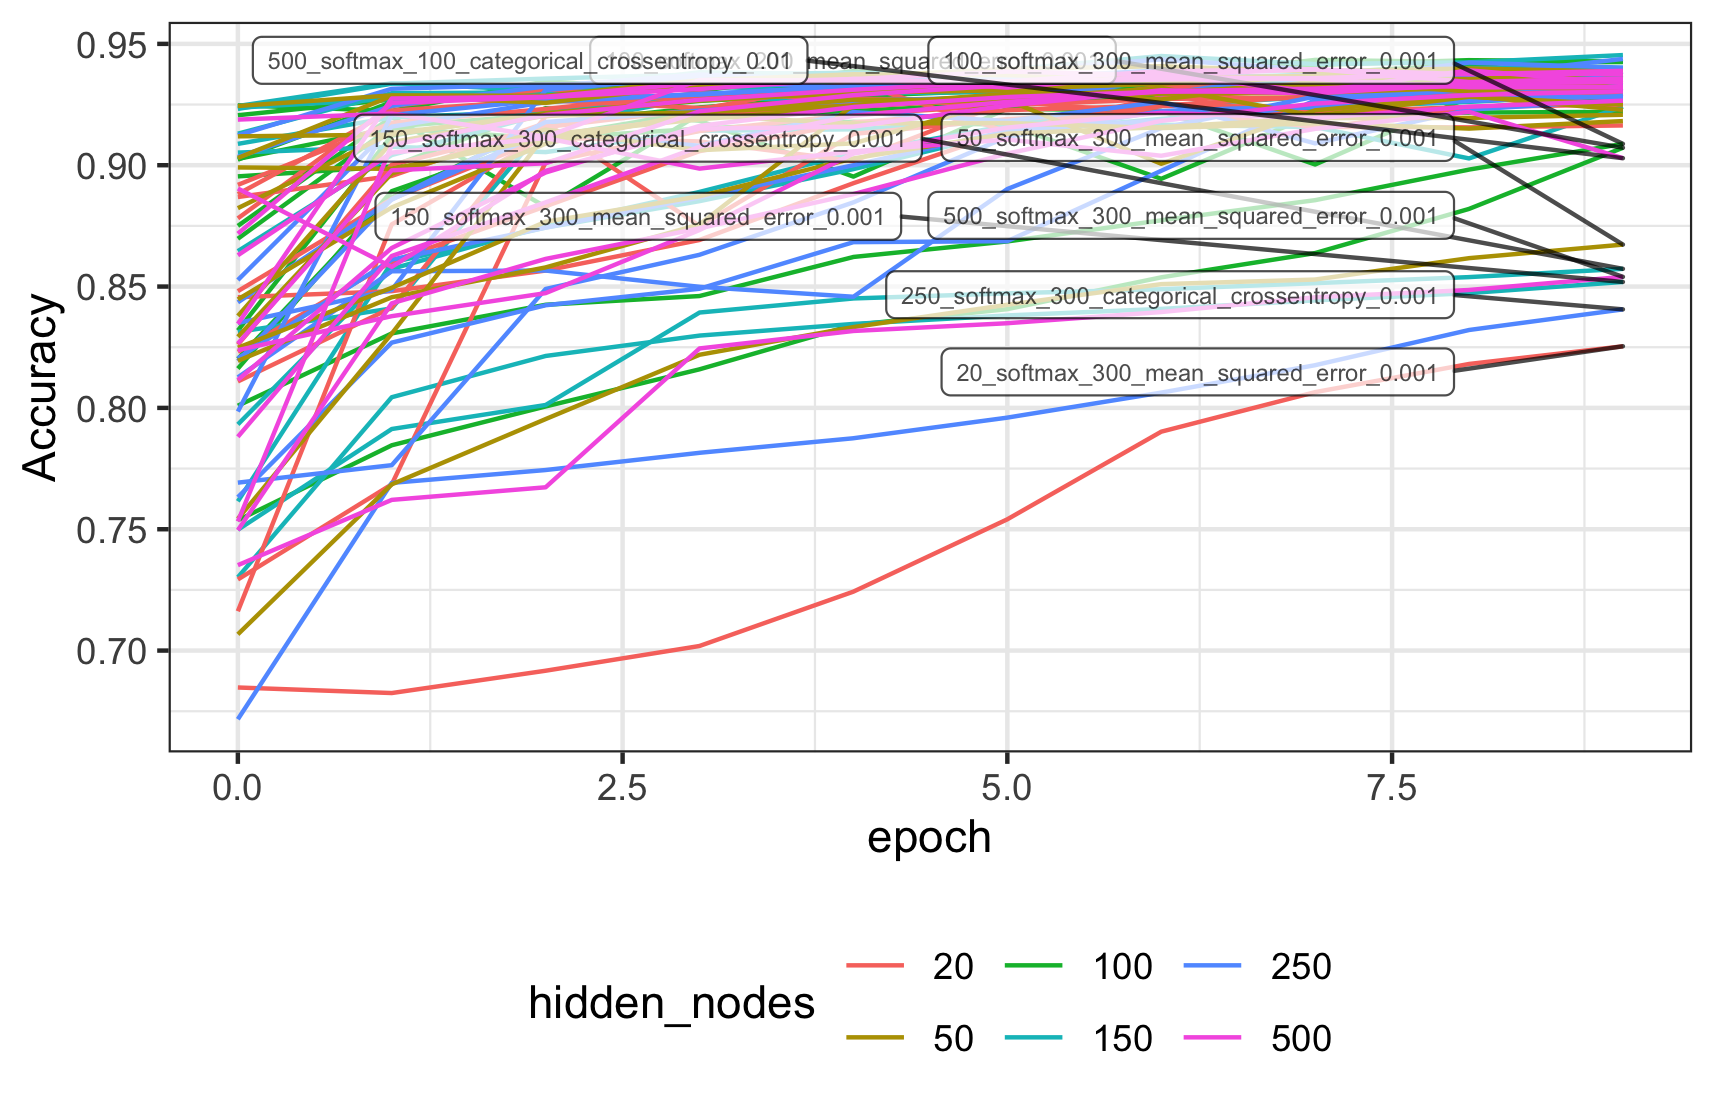
\includegraphics[width=0.8\textwidth]{figure/1-layer Neural Network Test Accuracy By Epoch.png}}
\caption{1-layer Neural Network Test Accuracy By Epoch}
\label{1-layer Neural Network Test Accuracy By Epoch}
\vspace{-1.5em}
\end{figure}


Next, we tune all the hyper-parameters. From Fig. \ref{1-Hidden Layer Neural Network Accuracy rate versus bias}, we can see that bias barely improves accuracy.
\begin{figure}[htbp]
\centerline{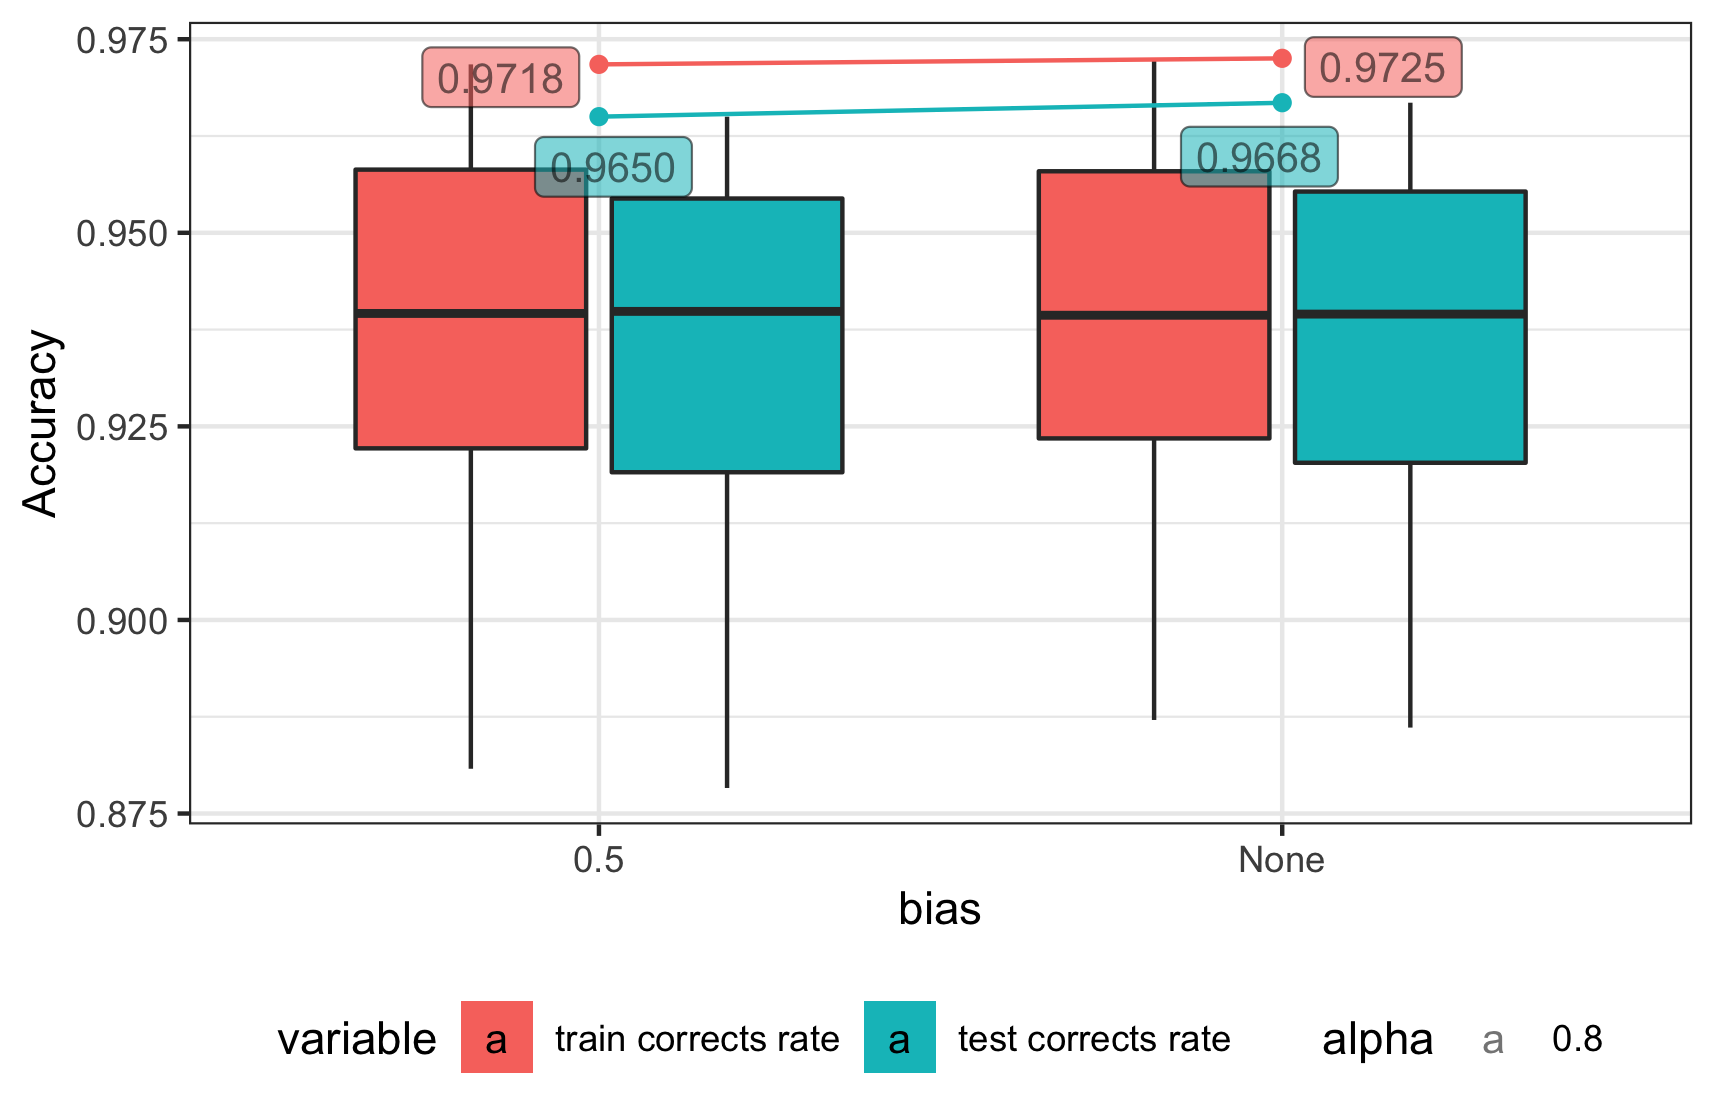
\includegraphics[width=0.8\textwidth]{figure/1-Hidden Layer Neural Network Accuracy rate versus bias.png}}
\caption{1-Hidden Layer NN Accuracy rate versus bias(Softmax)}
\label{1-Hidden Layer Neural Network Accuracy rate versus bias}
\vspace{-1.5em}
\end{figure}

From Fig. \ref{1-Hidden Layer Neural Network Accuracy rate versus hidden nodes}, we can see that a lager number of hidden nodes tends to have better accuracy. However, the best test accuracy is when number of hidden nodes equals 150.
\begin{figure}[htbp]
\centerline{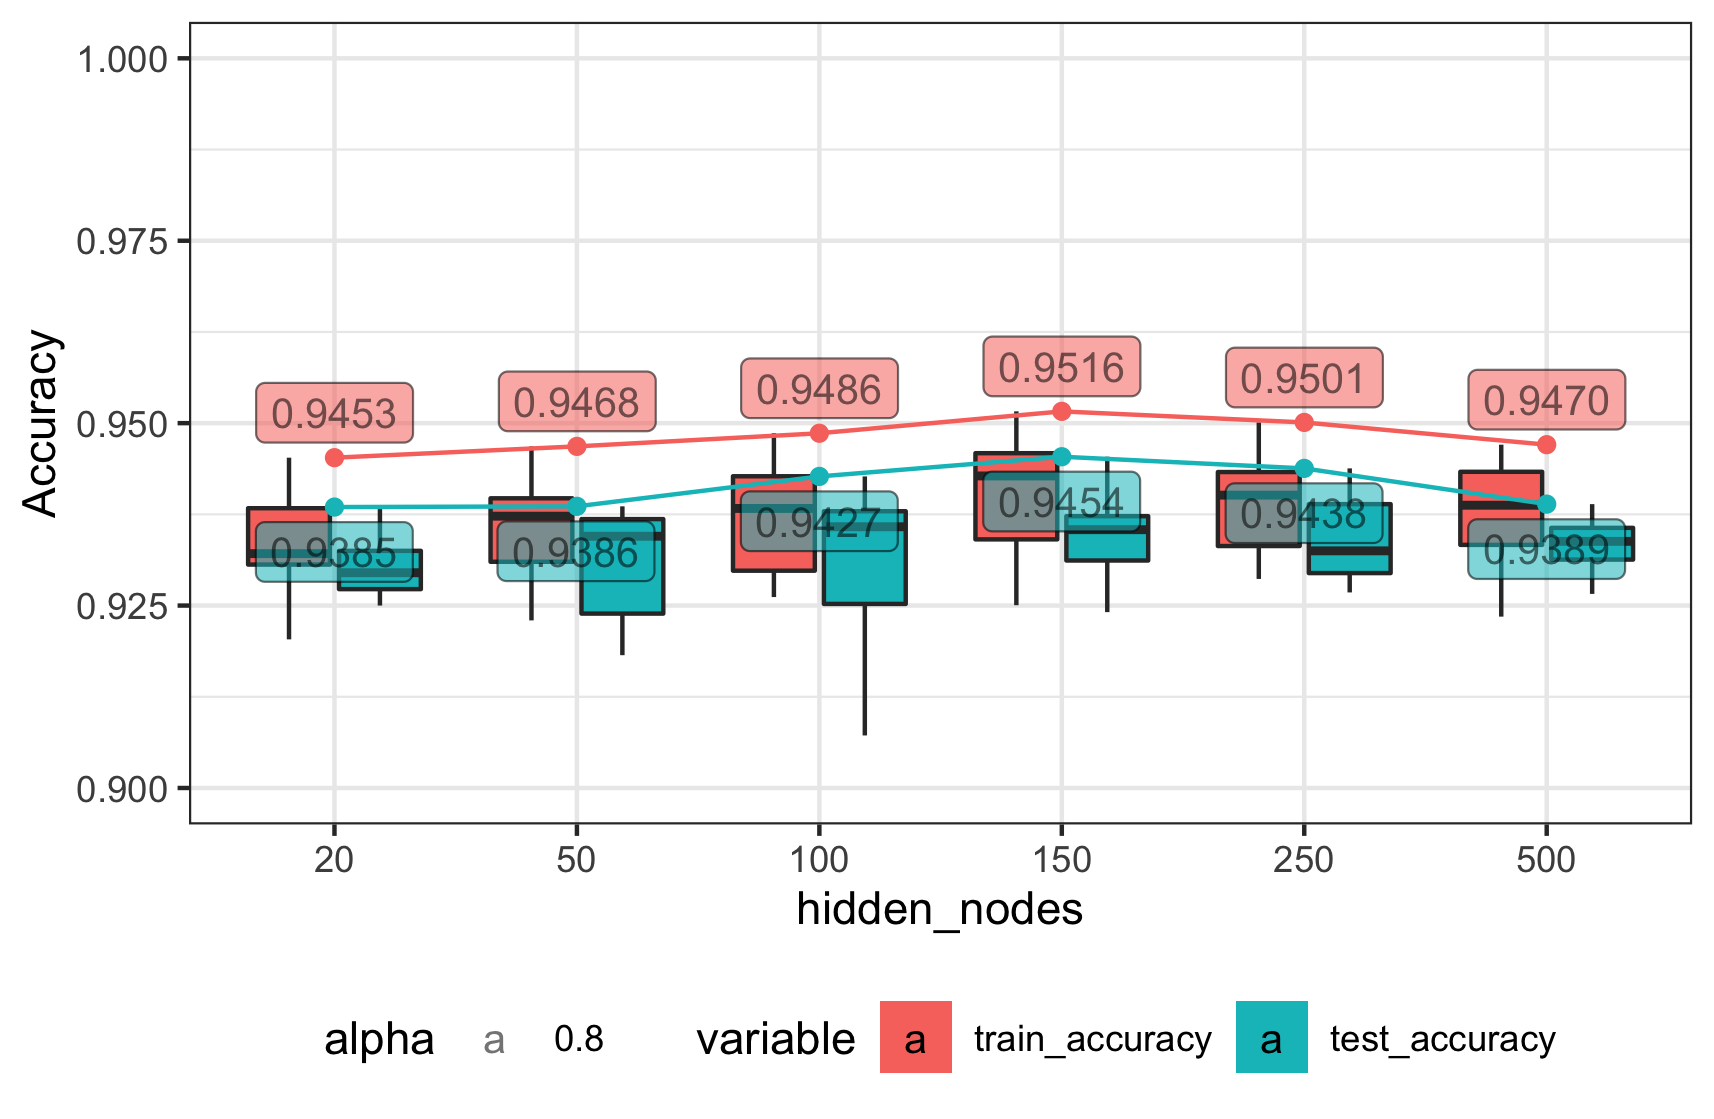
\includegraphics[width=0.8\textwidth]{figure/1-Hidden Layer Neural Network Accuracy rate versus hidden_nodes.png}}
\caption{1-Hidden Layer NN Accuracy rate versus hidden nodes(Softmax)}
\label{1-Hidden Layer Neural Network Accuracy rate versus hidden nodes}
\vspace{-1.5em}
\end{figure}

From Fig. \ref{1-Hidden Layer Neural Network Accuracy rate versus learning rate}\footnote{Besides, we also used a learning rate of 0.1. However, the accuracy of training result was trapped around 10\%, which means that a learning rate of 0.1 skipped the best parameter. Therefore, we didn't show the box plot of 0.1 learning rate here.}, we can see that a learning rate of $0.01$ tends to have better accuracy than 0.001. 
\begin{figure}[htbp]
\centerline{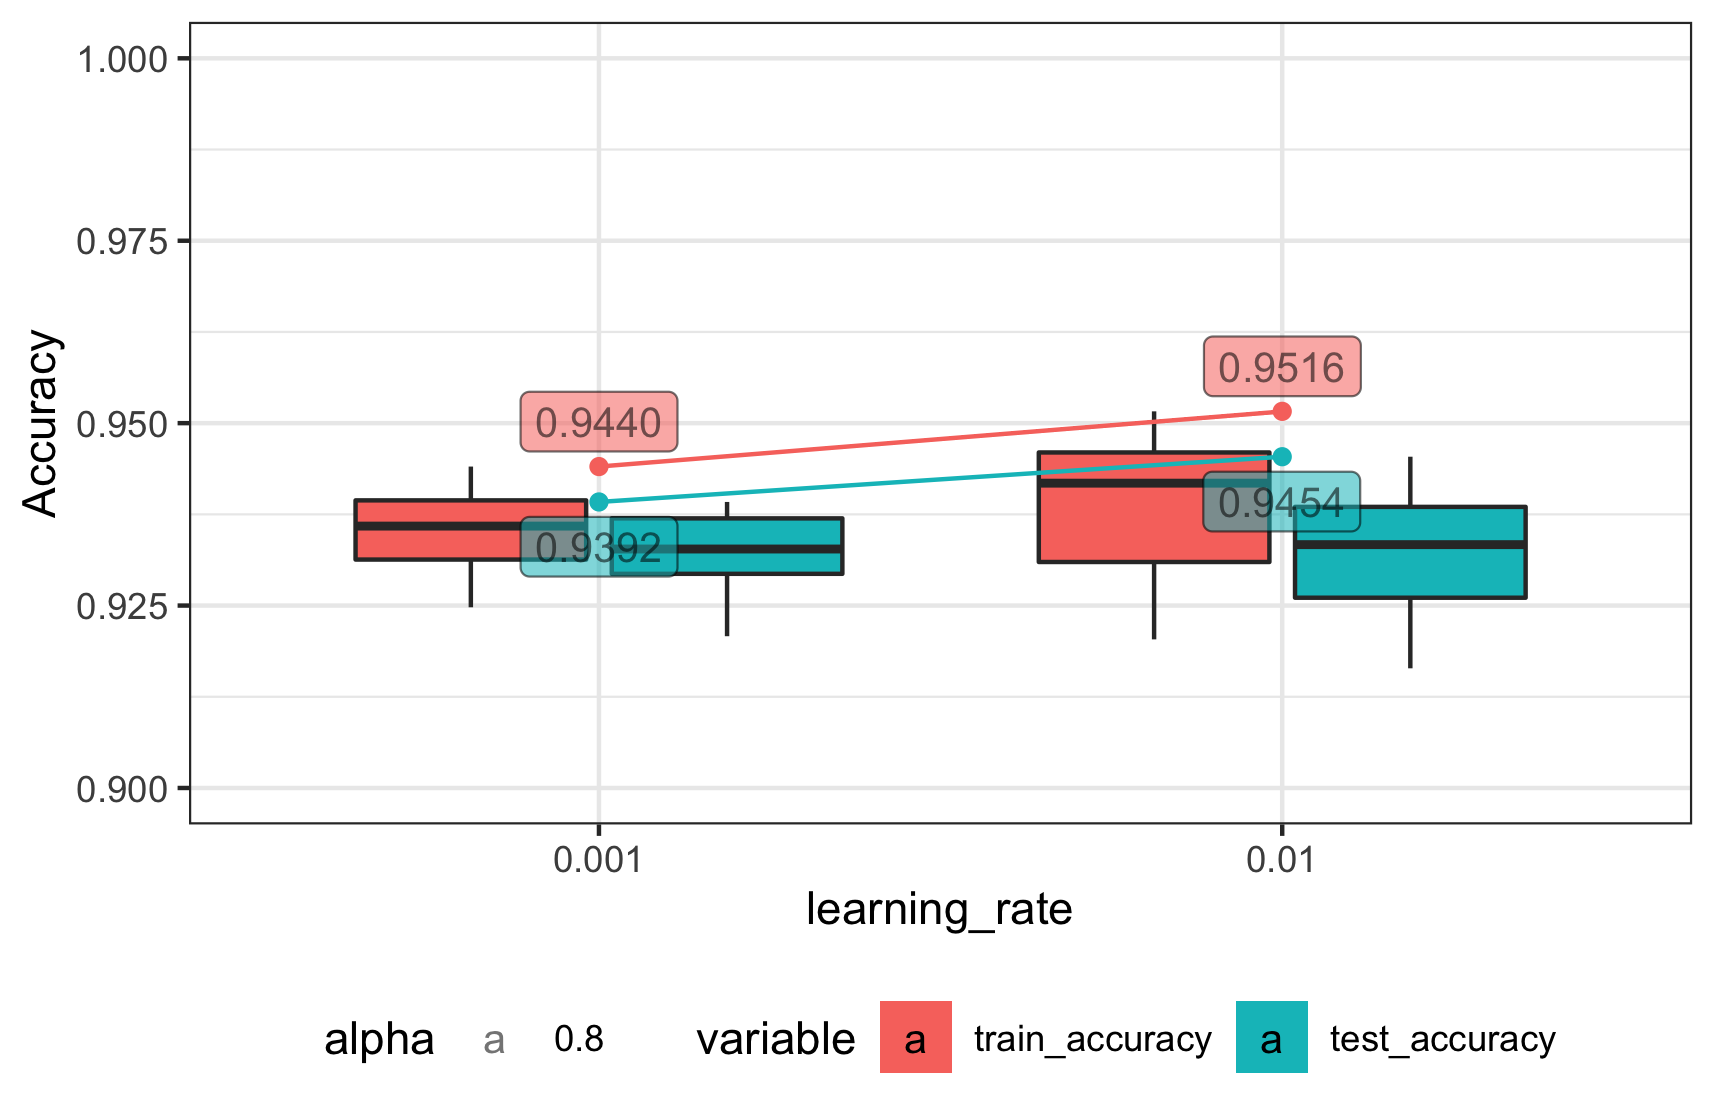
\includegraphics[width=0.8\textwidth]{figure/1-Hidden Layer Neural Network Accuracy rate versus learning_rate.png}}
\caption{1-Hidden Layer NN Accuracy rate versus learning rate(Softmax)}
\label{1-Hidden Layer Neural Network Accuracy rate versus learning rate}
\vspace{-1.5em}
\end{figure}

From Fig. \ref{1-Hidden Layer Neural Network Accuracy rate versus loss}, we can see that a the use of different loss function don't impact the test accuracy a lot.
\begin{figure}[htbp]
\centerline{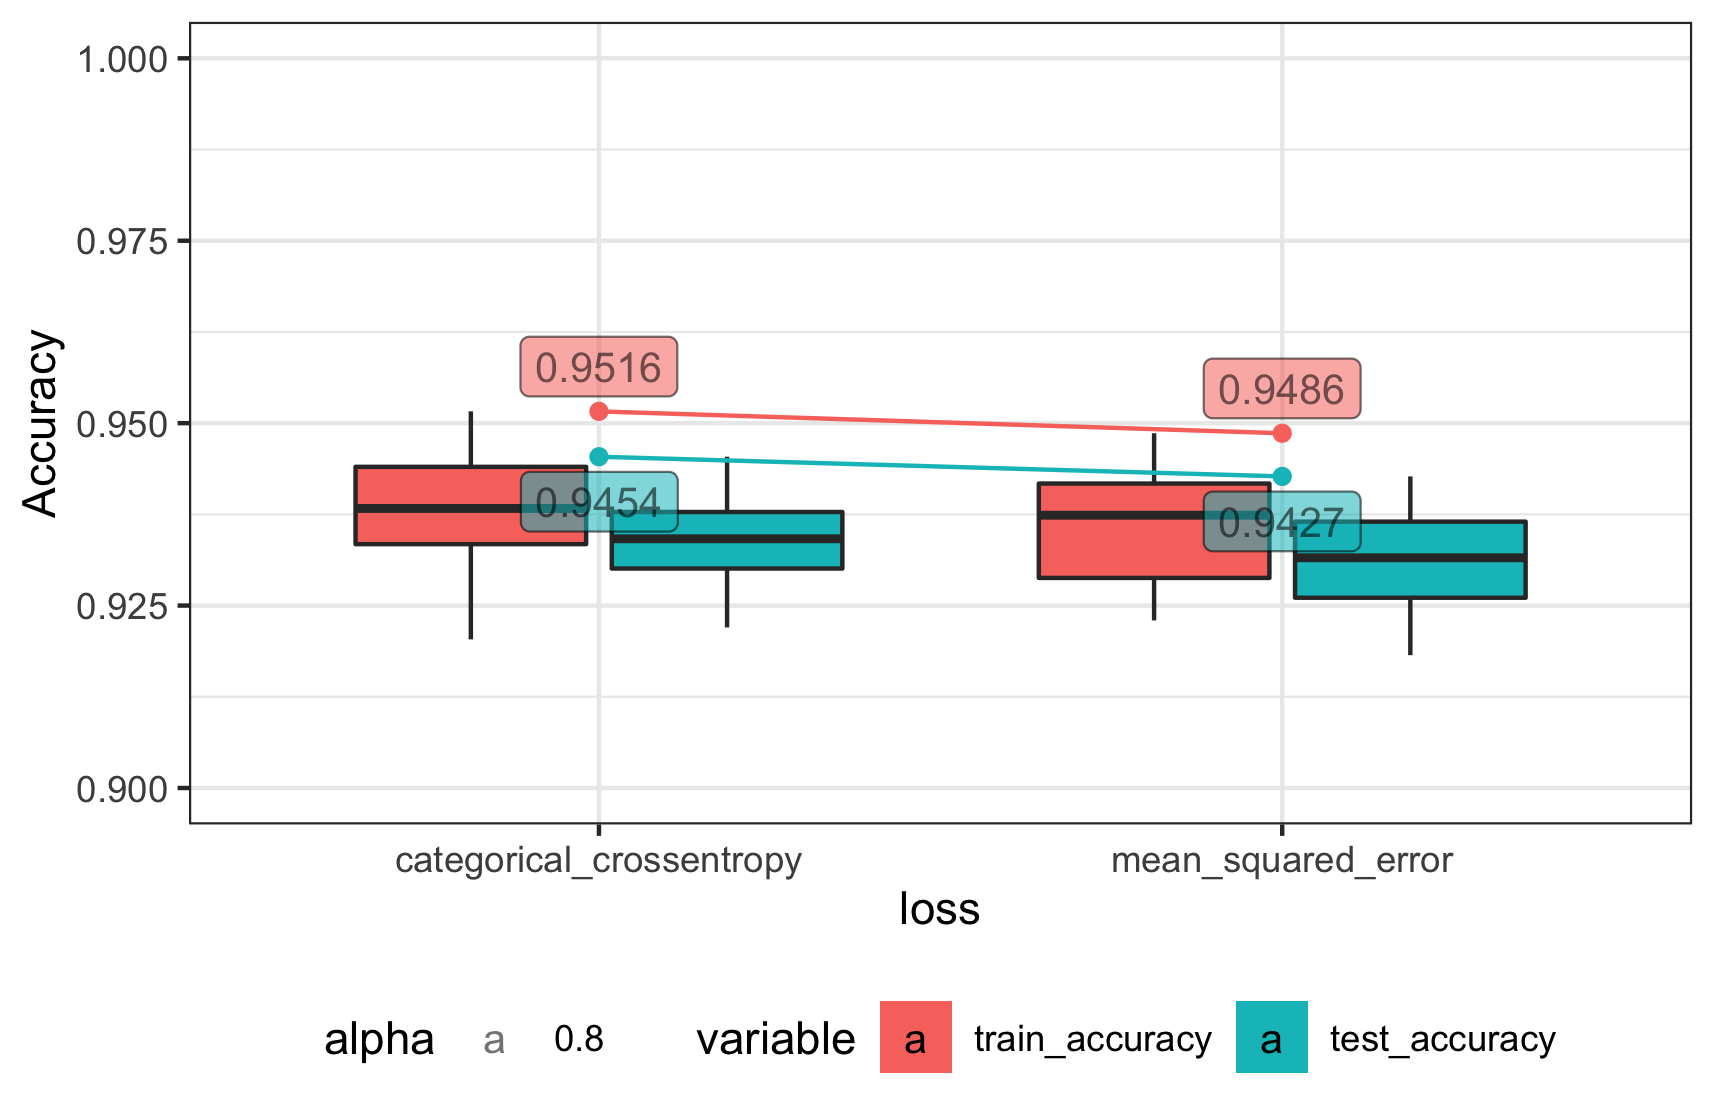
\includegraphics[width=0.8\textwidth]{figure/1-Hidden Layer Neural Network Accuracy rate versus loss.png}}
\caption{1-Hidden Layer NN Accuracy rate versus loss(Softmax)}
\label{1-Hidden Layer Neural Network Accuracy rate versus loss}
\vspace{-1.5em}
\end{figure}

\begin{figure}[htbp]
\centerline{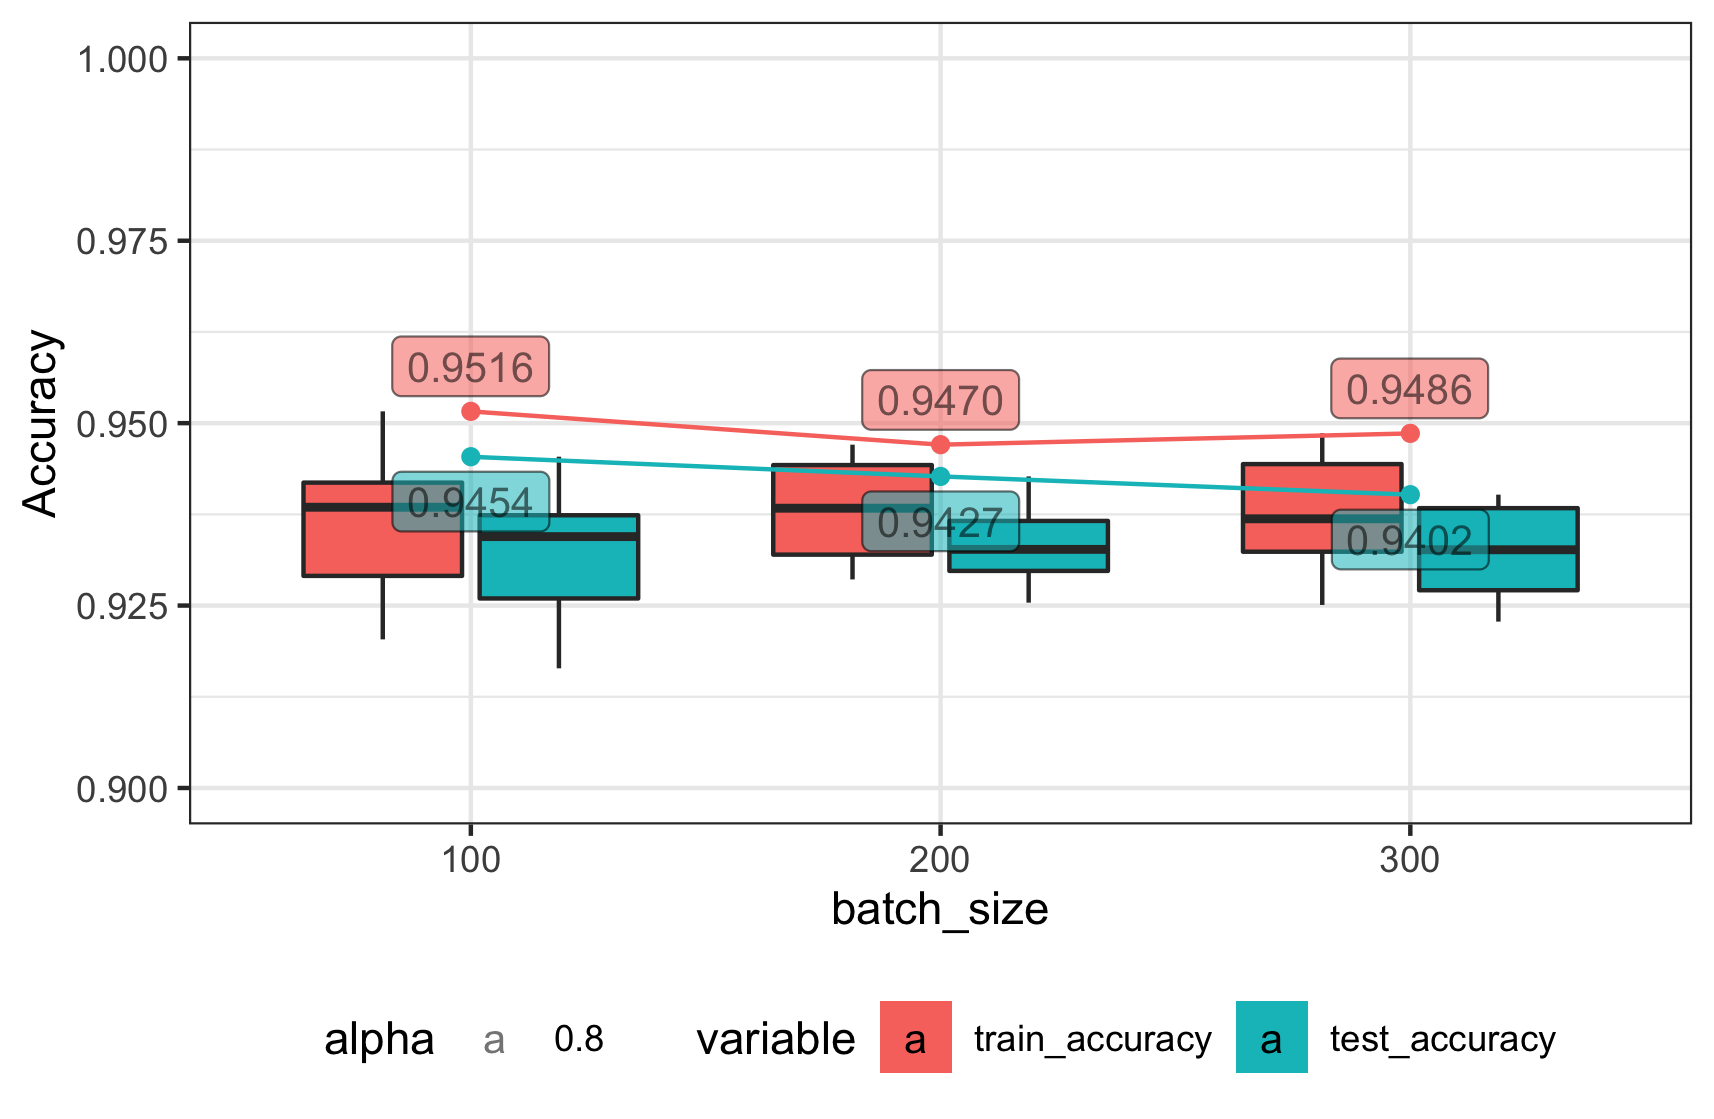
\includegraphics[width=0.8\textwidth]{figure/1-Hidden Layer Neural Network Accuracy rate versus batch_size.png}}
\caption{1-Hidden Layer NN Accuracy rate versus batch size(Softmax)}
\label{1-Hidden Layer Neural Network Accuracy rate batch size loss}
\vspace{-1.5em}
\end{figure}



We pick the model of best test accuracy, whose details are as in TABLE \ref{1-layer Neutral Network best hyper-parameter(softmax)} and the confusion table is as TABLE \ref{1-layer Neutral Network confusion table(softmax)}.
% latex table generated in R 3.5.2 by xtable 1.8-4 package
% Mon Apr 13 03:32:32 2020
\begin{table}[htbp]
\tiny
\centering
\caption{1-layer Neutral Network best hyper-parameter(softmax)}
\begin{tabular}{|c|c|c|c|}
  \hline
 hidden\_nodes & activation & batch\_size & loss \\

 150 & softmax & 100 & categorical\_crossentropy \\
  \hline
 learning\_rate & epoch & variable & value \\ 

 0.01 &   9 & test\_accuracy & 0.9454 \\ 
   \hline
\end{tabular}
\label{1-layer Neutral Network best hyper-parameter(softmax)}	
\end{table}



% Table generated by Excel2LaTeX from sheet 'Sheet1'
\begin{table}[htbp]
\tiny
  \centering
  \caption{1-layer Neutral Network confusion table(softmax)}
% Table generated by Excel2LaTeX from sheet 'Sheet2'
\begin{tabular}{|r|rrrrrrrrrr|r|}
\hline
  & 0 & 1 & 2 & 3 & 4 & 5 & 6 & 7 & 8 & 9 &  \\
\hline
0 & 965 & 0 & 9 & 0 & 2 & 5 & 6 & 1 & 5 & 2 & 0.9698 \\
1 & 0 & 1126 & 4 & 0 & 0 & 1 & 4 & 8 & 4 & 6 & 0.9766 \\
2 & 0 & 4 & 998 & 7 & 1 & 1 & 1 & 22 & 3 & 1 & 0.9615 \\
3 & 1 & 1 & 5 & 977 & 0 & 10 & 0 & 10 & 23 & 9 & 0.9431 \\
4 & 0 & 0 & 2 & 2 & 952 & 2 & 5 & 3 & 7 & 12 & 0.9665 \\
5 & 3 & 1 & 0 & 10 & 0 & 853 & 13 & 0 & 7 & 1 & 0.9606 \\
6 & 4 & 1 & 3 & 1 & 9 & 7 & 924 & 0 & 3 & 1 & 0.9696 \\
7 & 1 & 1 & 7 & 4 & 0 & 2 & 0 & 966 & 5 & 5 & 0.9748 \\
8 & 1 & 1 & 3 & 3 & 1 & 8 & 5 & 1 & 909 & 1 & 0.9743 \\
9 & 5 & 0 & 1 & 6 & 17 & 3 & 0 & 17 & 8 & 971 & 0.9446 \\
\hline
  & 0.9847 & 0.9921 & 0.9671 & 0.9673 & 0.9695 & 0.9563 & 0.9645 & 0.9397 & 0.9333 & 0.9623 & 0.9454 \\
\hline
\end{tabular}%
  \label{1-layer Neutral Network confusion table(softmax)}%
\end{table}%
\end{frame}


















\subsubsection{ReLU activation function}
\begin{frame}[allowframebreaks]{\secname : \subsecname}{\subsubsecname}
ReLU stands for rectified linear unit, and is a type of activation function:
$$\sigma(\mathbf{z})_j=\max (0,\mathbf{z}_j)\quad \text { for } j=1, \ldots, K$$

Since we conclude bias term nearly have no affects in improving test accuracy in \ref{Softmax activation function}, we didn't consider bias term from now on. 

We trained 108 1-layer Neutral Network models with different hidden nodes, learning rates and bias, for every type of model we trained 10 epochs. The hyper-parameter field are as follows, which are the same as the hyper-parameter field of 1-hidden layer neural networks with softmax activation function.
\begin{itemize}
  \item Number of hidden nodes: 20, 50, 100, 150, 250, 500;
  \item batch size: 100, 200, 300;
  \item loss function: mean squared error, categorical cross-entropy;
  \item Learning rate: 0.001, 0.01, 0.1.
\end{itemize}

\framebreak
First, we need to know if all our model is converged. From Fig. \ref{1-layer Neural Network Test Accuracy By Epoch(ReLU)}, we can see that all of our models are converged. Besides, we can also see that those different group of model's iteration lines are approximately parallel, which implies that ReLU activation function can update the parameter more correctly, compared to Fig. \ref{1-layer Neural Network Test Accuracy By Epoch}.
\begin{figure}[htbp]
\centerline{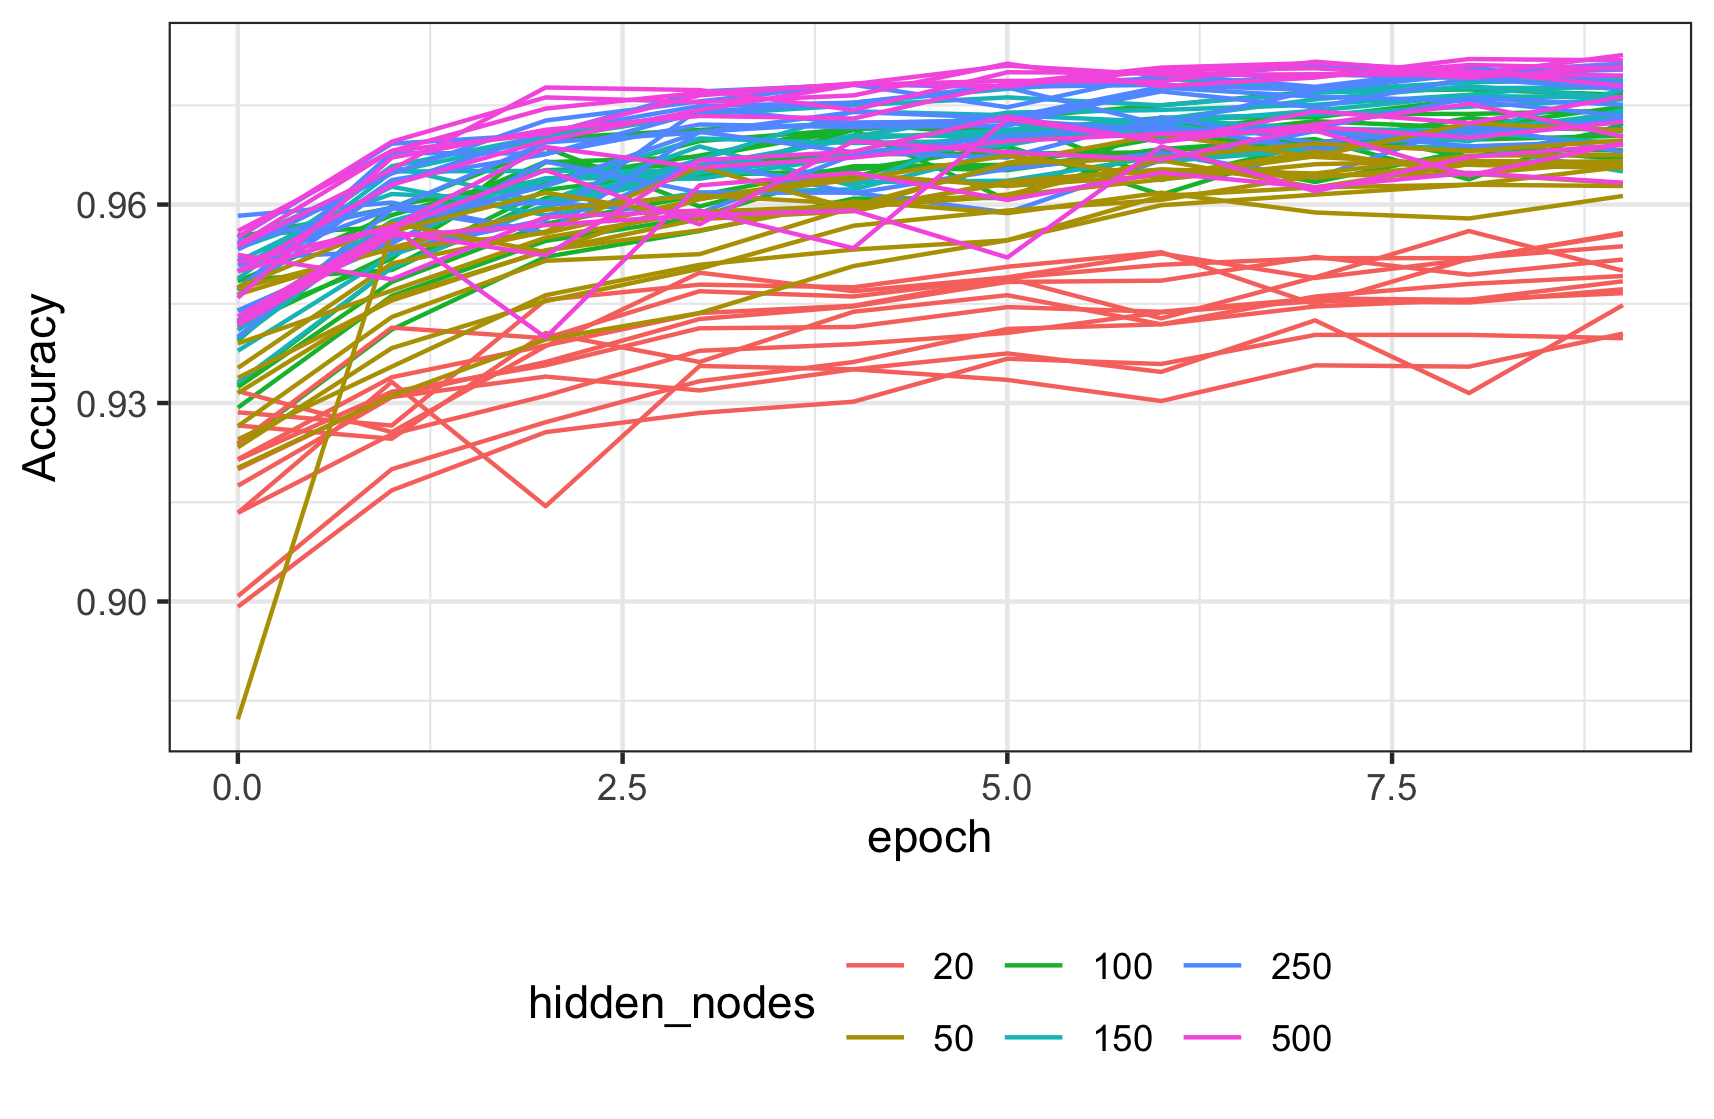
\includegraphics[width=0.7\textwidth]{figure/91-layer Neural Network Test Accuracy By Epoch.png}}
\caption{1-layer Neural Network Test Accuracy By Epoch(ReLU)}
\label{1-layer Neural Network Test Accuracy By Epoch(ReLU)}
\vspace{-1.5em}
\end{figure}


Next, we tune all the hyper-parameters. From Fig. \ref{1-Hidden Layer Neural Network Accuracy rate versus hidden nodes(ReLU)}, we can see that the more hidden nodes, the better the maximum test accuracy is.
\begin{figure}[htbp]
\centerline{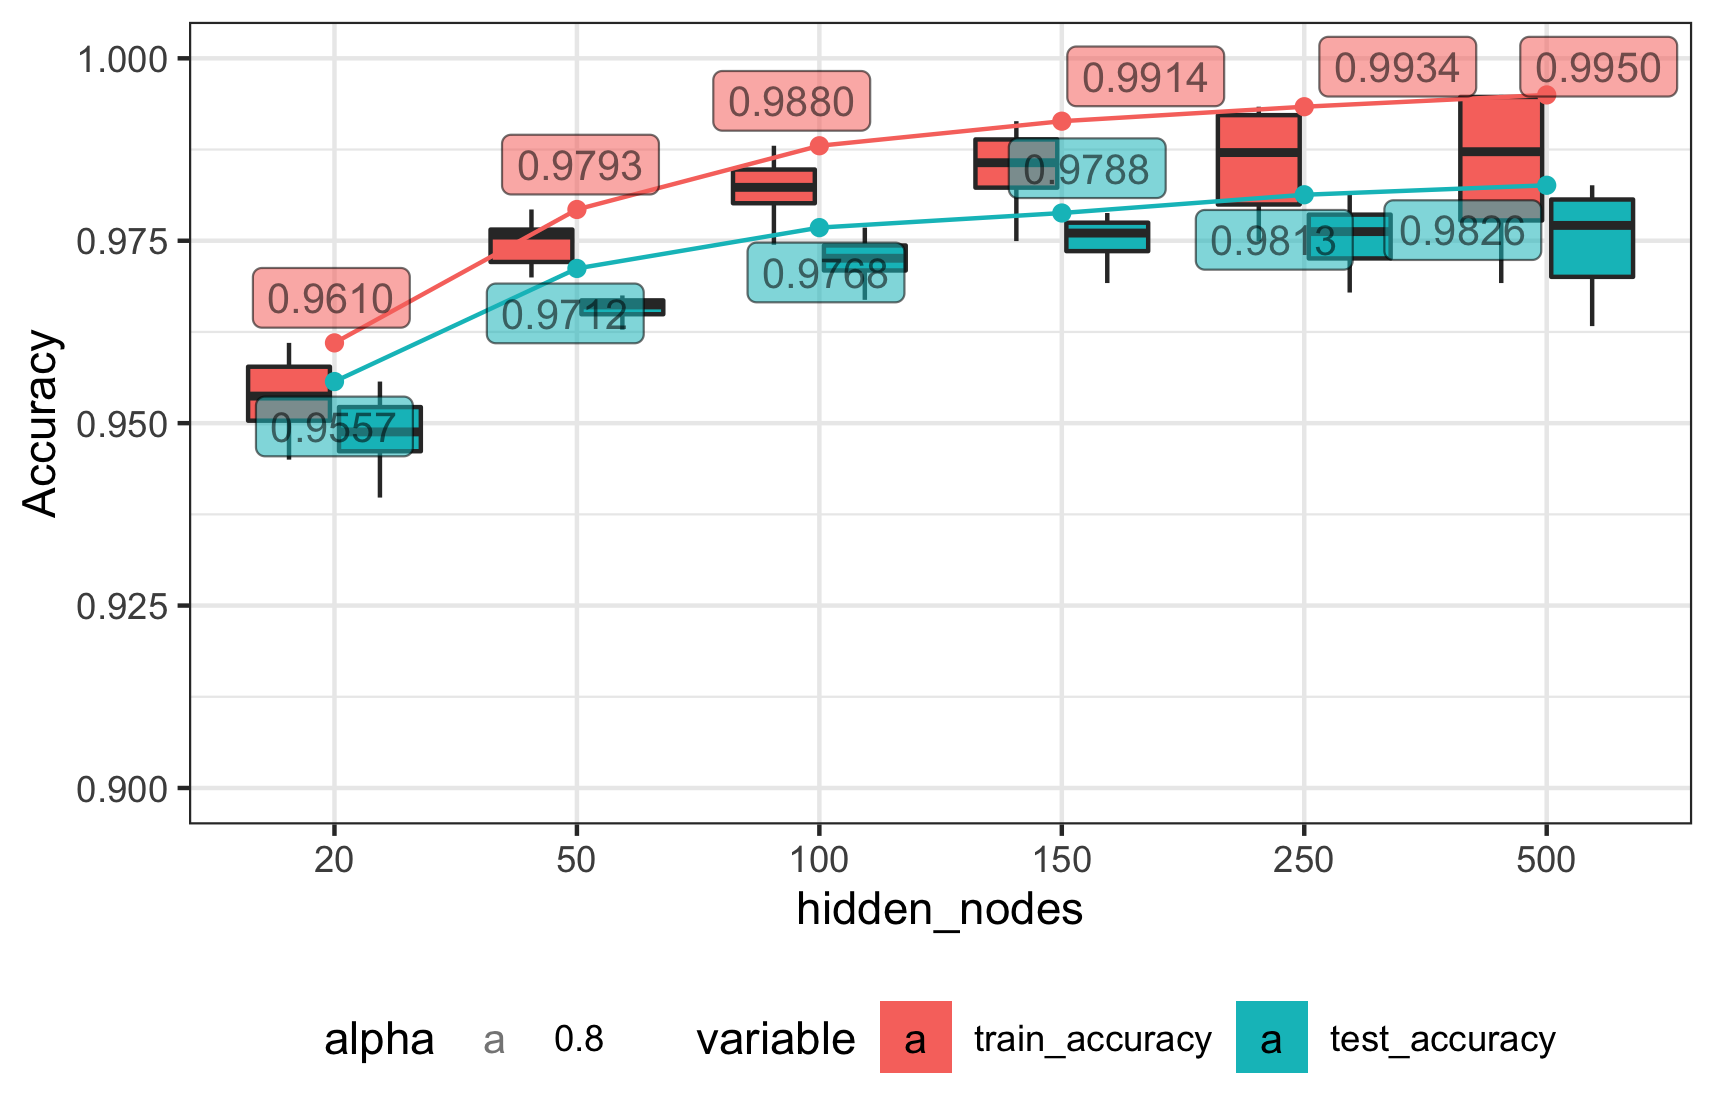
\includegraphics[width=0.8\textwidth]{figure/91-Hidden Layer Neural Network Accuracy rate versus hidden_nodes.png}}
\caption{1-Hidden Layer NN Accuracy rate versus hidden nodes(ReLU)}
\label{1-Hidden Layer Neural Network Accuracy rate versus hidden nodes(ReLU)}
\vspace{-1.5em}
\end{figure}

From Fig. \ref{1-Hidden Layer Neural Network Accuracy rate versus learning rate(ReLU)}, we can see that a learning rate of 0.001 is better than 0.01. Besides, we also used a learning rate of 0.1. However, the accuracy of training result was trapped around 10\%, which means that a learning rate of 0.1 skipped the best parameter. Therefore, we didn't show the box plot of 0.1 learning rate here.
\begin{figure}[htbp]
\centerline{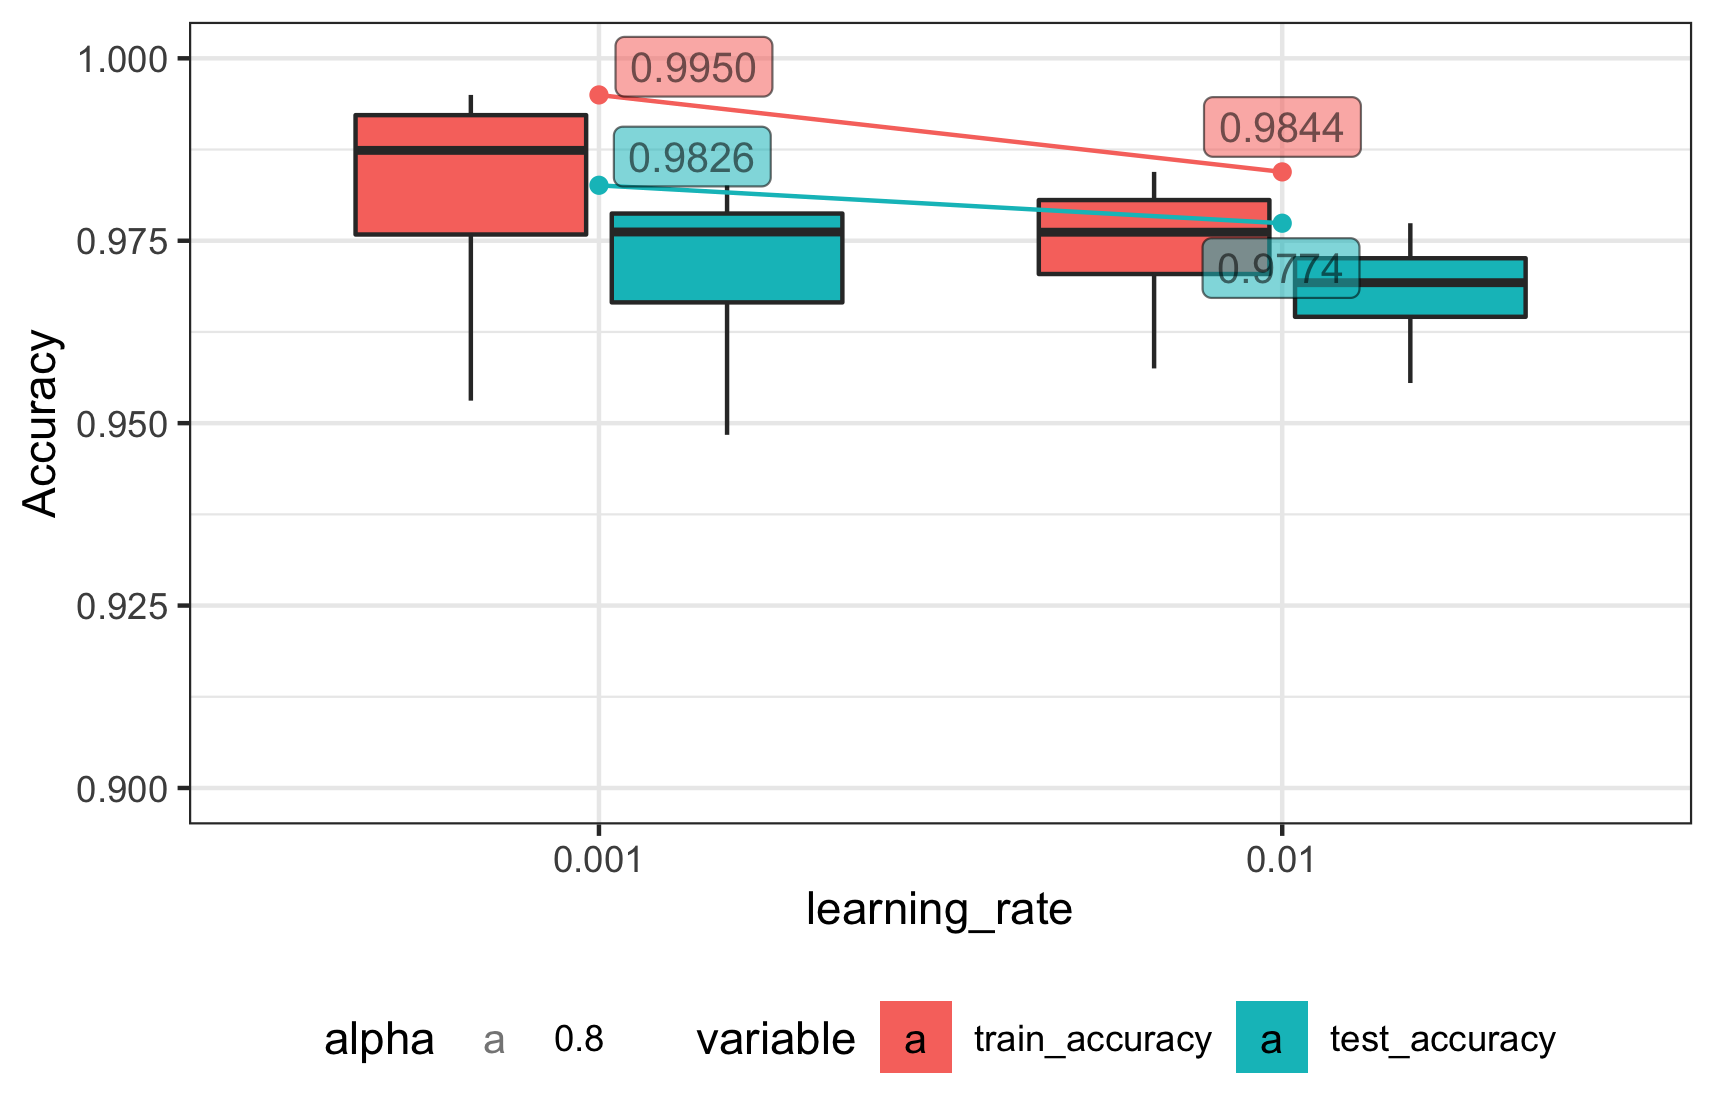
\includegraphics[width=0.8\textwidth]{figure/91-Hidden Layer Neural Network Accuracy rate versus learning_rate.png}}
\caption{1-Hidden Layer Neural Network Accuracy rate versus learning rate(ReLU)}
\label{1-Hidden Layer Neural Network Accuracy rate versus learning rate(ReLU)}
\vspace{-1.5em}
\end{figure}

From Fig. \ref{1-Hidden Layer Neural Network Accuracy rate versus loss(ReLU)}, we conclude loss function barely impact accuracy.
\begin{figure}[htbp]
\centerline{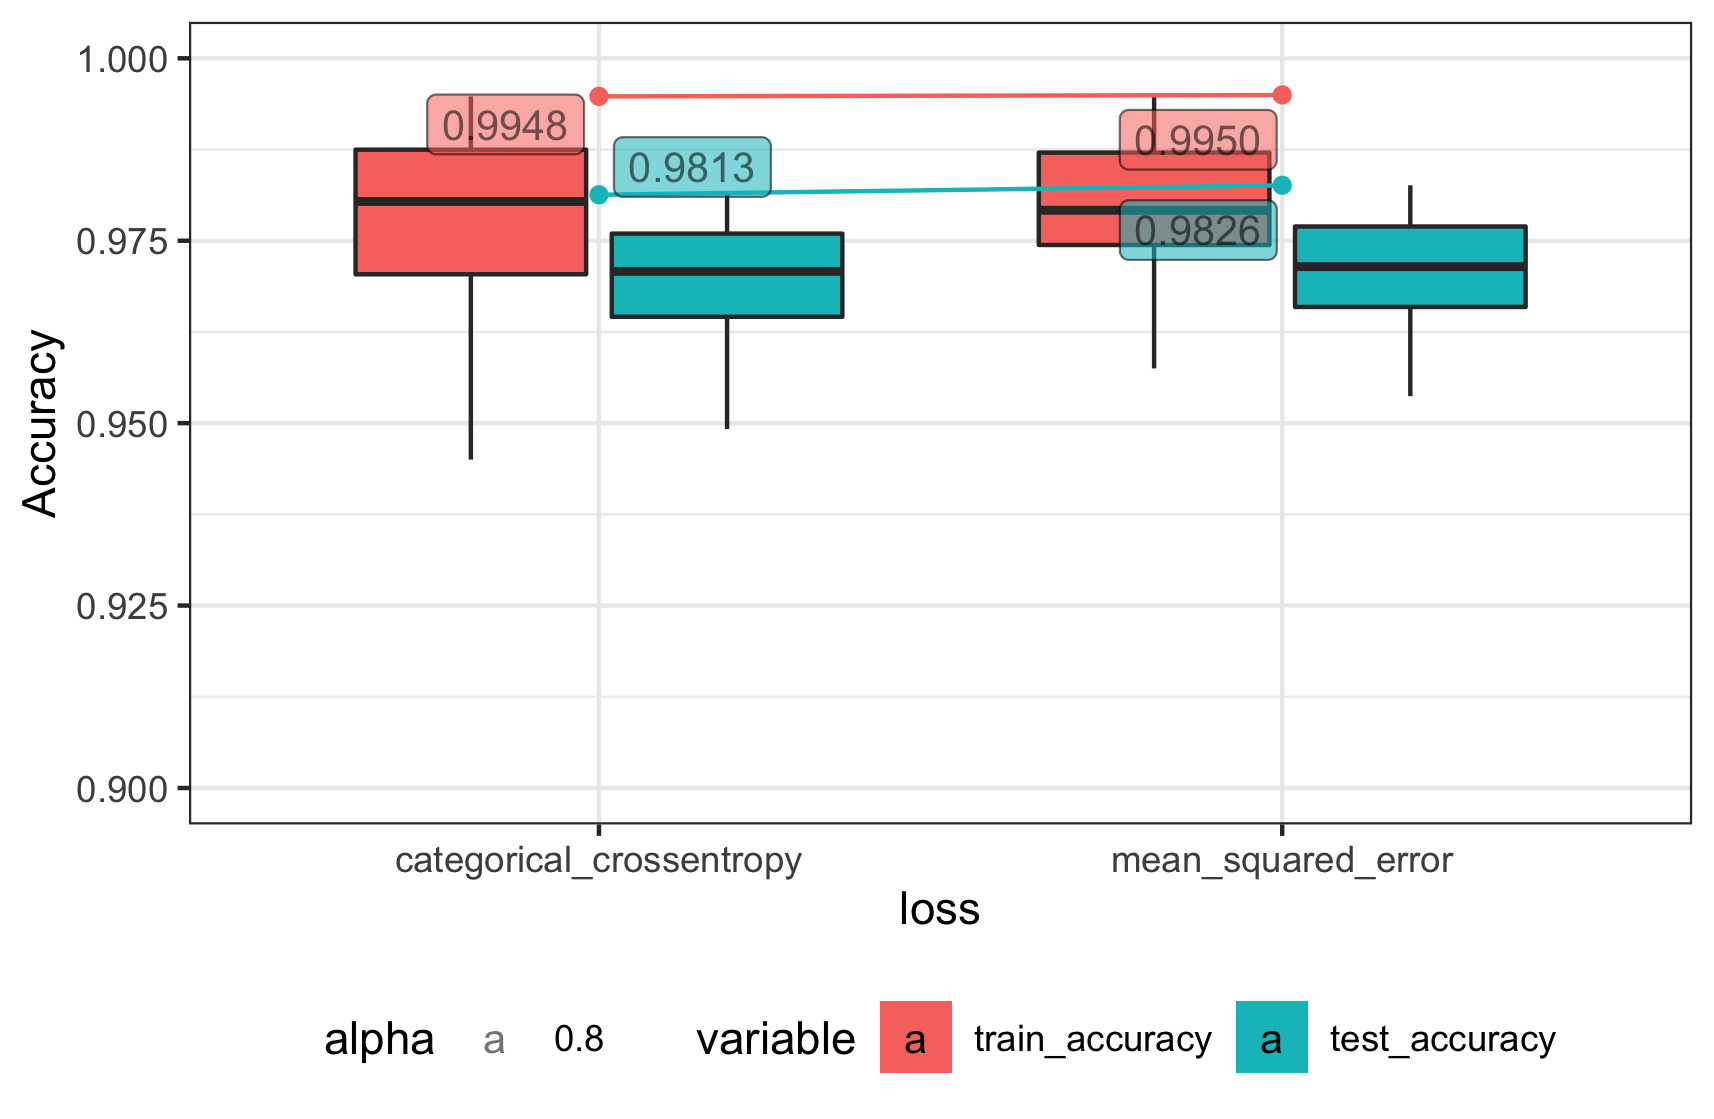
\includegraphics[width=0.8\textwidth]{figure/91-Hidden Layer Neural Network Accuracy rate versus loss.png}}
\caption{1-Hidden Layer NN Accuracy rate versus loss(ReLU)}
\label{1-Hidden Layer Neural Network Accuracy rate versus loss(ReLU)}
\vspace{-1.5em}
\end{figure}

From Fig. \ref{1-Hidden Layer Neural Network Accuracy rate versus batch size(ReLU)}, we conclude batch size barely impact accuracy.
\begin{figure}[htbp]
\centerline{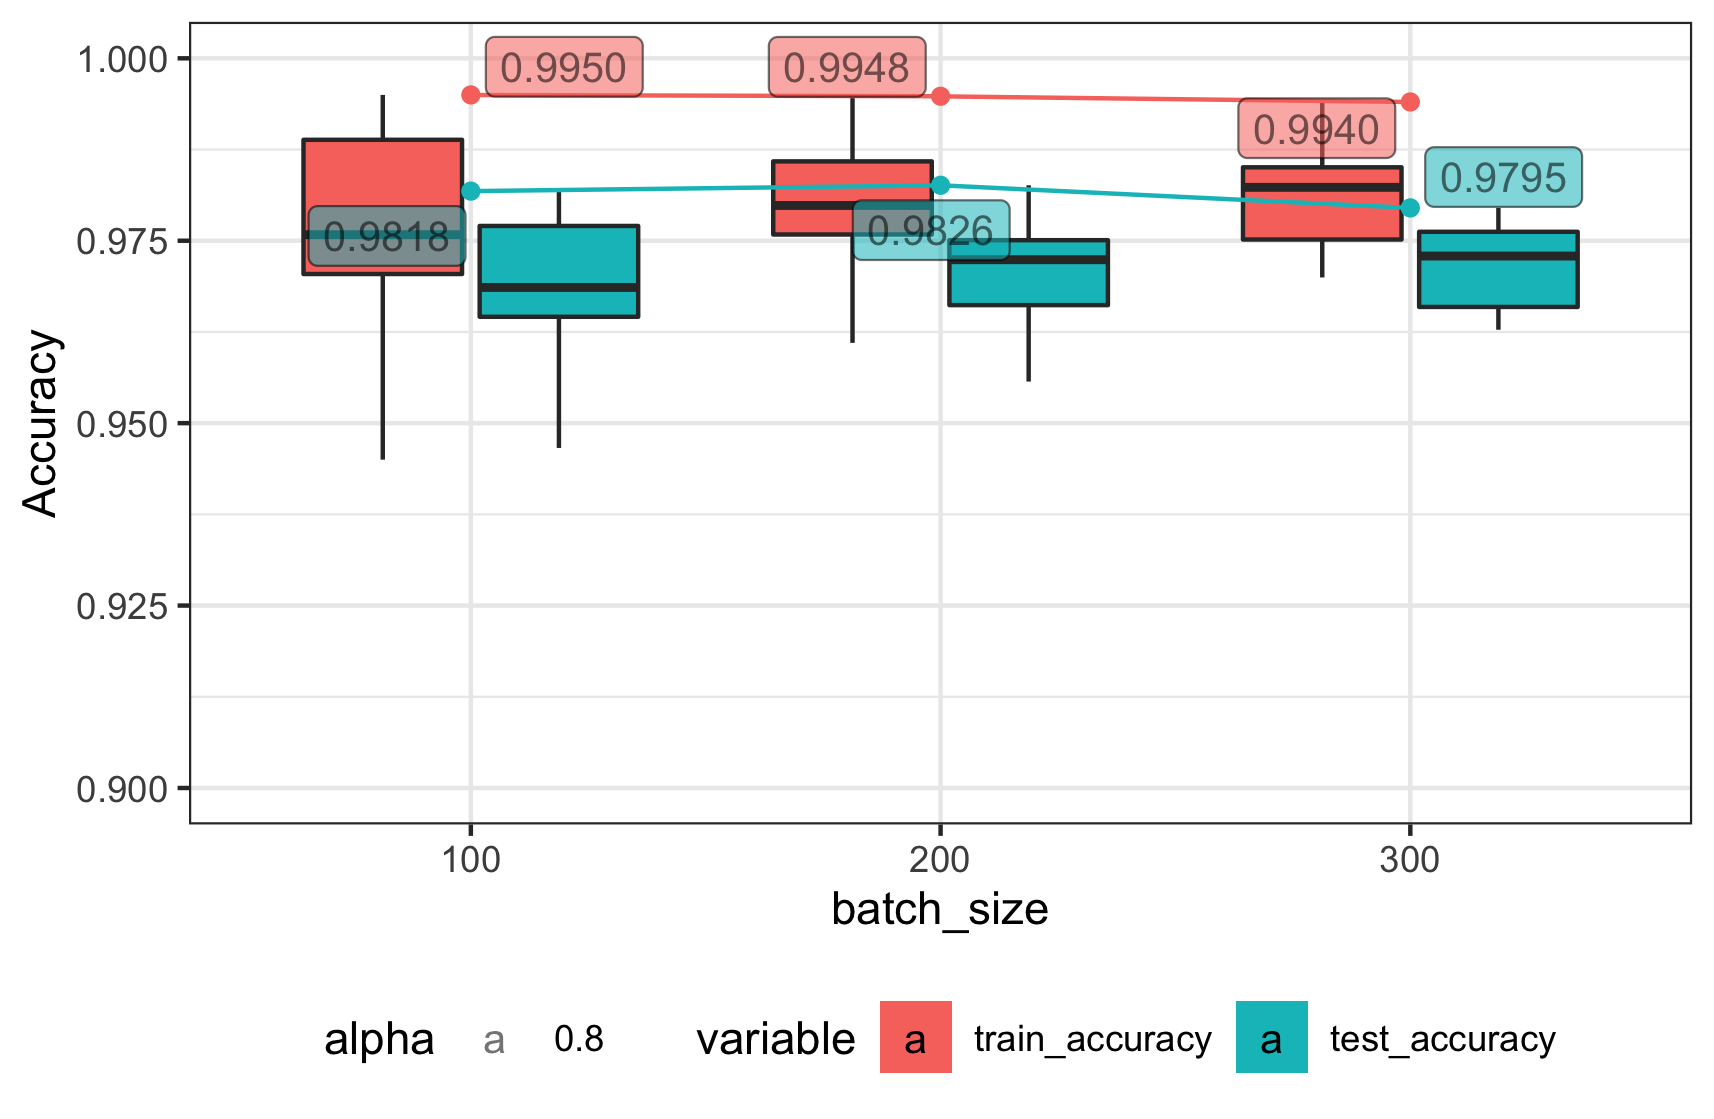
\includegraphics[width=0.8\textwidth]{figure/91-Hidden Layer Neural Network Accuracy rate versus batch_size.png}}
\caption{1-Hidden Layer NN Accuracy rate versus batch size(ReLU)}
\label{1-Hidden Layer Neural Network Accuracy rate versus batch size(ReLU)}
\vspace{-1.5em}
\end{figure}



We pick the model of best test accuracy, whose details are as in TABLE \ref{1-layer Neutral Network best hyper-parameter(ReLU)} and the confusion table is as TABLE \ref{1-layer Neutral Network confusion table(ReLU)}.
% latex table generated in R 3.5.2 by xtable 1.8-4 package
% Mon Apr 13 03:32:32 2020
\begin{table}[htbp]
\tiny
\centering
\caption{1-layer Neutral Network best hyper-parameter(ReLU)}
\begin{tabular}{|c|c|c|c|}
  \hline
 hidden\_nodes & activation & batch\_size & loss \\

 500 & ReLU & 200 & mean\_squared\_error \\
  \hline
 learning\_rate & epoch & variable & value \\ 

 0.001 &   10 & test\_accuracy & 0.9826 \\ 
   \hline
\end{tabular}
\label{1-layer Neutral Network best hyper-parameter(ReLU)}	
\end{table}



% Table generated by Excel2LaTeX from sheet 'Sheet1'
\begin{table}[htbp]
\tiny
  \centering
  \caption{1-layer Neutral Network confusion table(ReLU)}
% Table generated by Excel2LaTeX from sheet 'Sheet2'
\begin{tabular}{|r|rrrrrrrrrr|r|}
\hline
  & 0 & 1 & 2 & 3 & 4 & 5 & 6 & 7 & 8 & 9 &  \\
\hline
0 & 971 & 0 & 0 & 1 & 0 & 5 & 0 & 1 & 2 & 0 & 0.9908 \\
1 & 0 & 1126 & 3 & 2 & 0 & 0 & 2 & 1 & 1 & 0 & 0.9921 \\
2 & 1 & 1 & 1018 & 4 & 0 & 0 & 1 & 4 & 3 & 0 & 0.9864 \\
3 & 0 & 0 & 2 & 996 & 0 & 5 & 0 & 3 & 1 & 3 & 0.9861 \\
4 & 0 & 0 & 5 & 1 & 960 & 2 & 5 & 1 & 0 & 8 & 0.9776 \\
5 & 1 & 0 & 0 & 4 & 0 & 885 & 1 & 0 & 1 & 0 & 0.9922 \\
6 & 4 & 2 & 1 & 1 & 2 & 10 & 937 & 0 & 1 & 0 & 0.9781 \\
7 & 1 & 2 & 8 & 3 & 0 & 1 & 0 & 1005 & 3 & 5 & 0.9776 \\
8 & 2 & 0 & 6 & 6 & 3 & 8 & 3 & 5 & 939 & 2 & 0.9641 \\
9 & 1 & 2 & 2 & 12 & 7 & 10 & 0 & 4 & 3 & 968 & 0.9594 \\
\hline
  & 0.9898 & 0.9938 & 0.9742 & 0.9670 & 0.9877 & 0.9557 & 0.9874 & 0.9814 & 0.9843 & 0.9817 & 0.9826 \\
\hline
\end{tabular}%
\label{1-layer Neutral Network confusion table(ReLU)}%
\end{table}%
\end{frame}


\subsubsection{Comparison}
\begin{frame}[allowframebreaks]{\secname : \subsecname}{\subsubsecname}
Now we compare the result of softmax activation function and ReLU activation function.

From Fig. \ref{1-Hidden Layer Neural Network Accuracy rate versus activation}, we can see that ReLU activation greatly improved the overall accuracy.
\begin{figure}[htbp]
\centerline{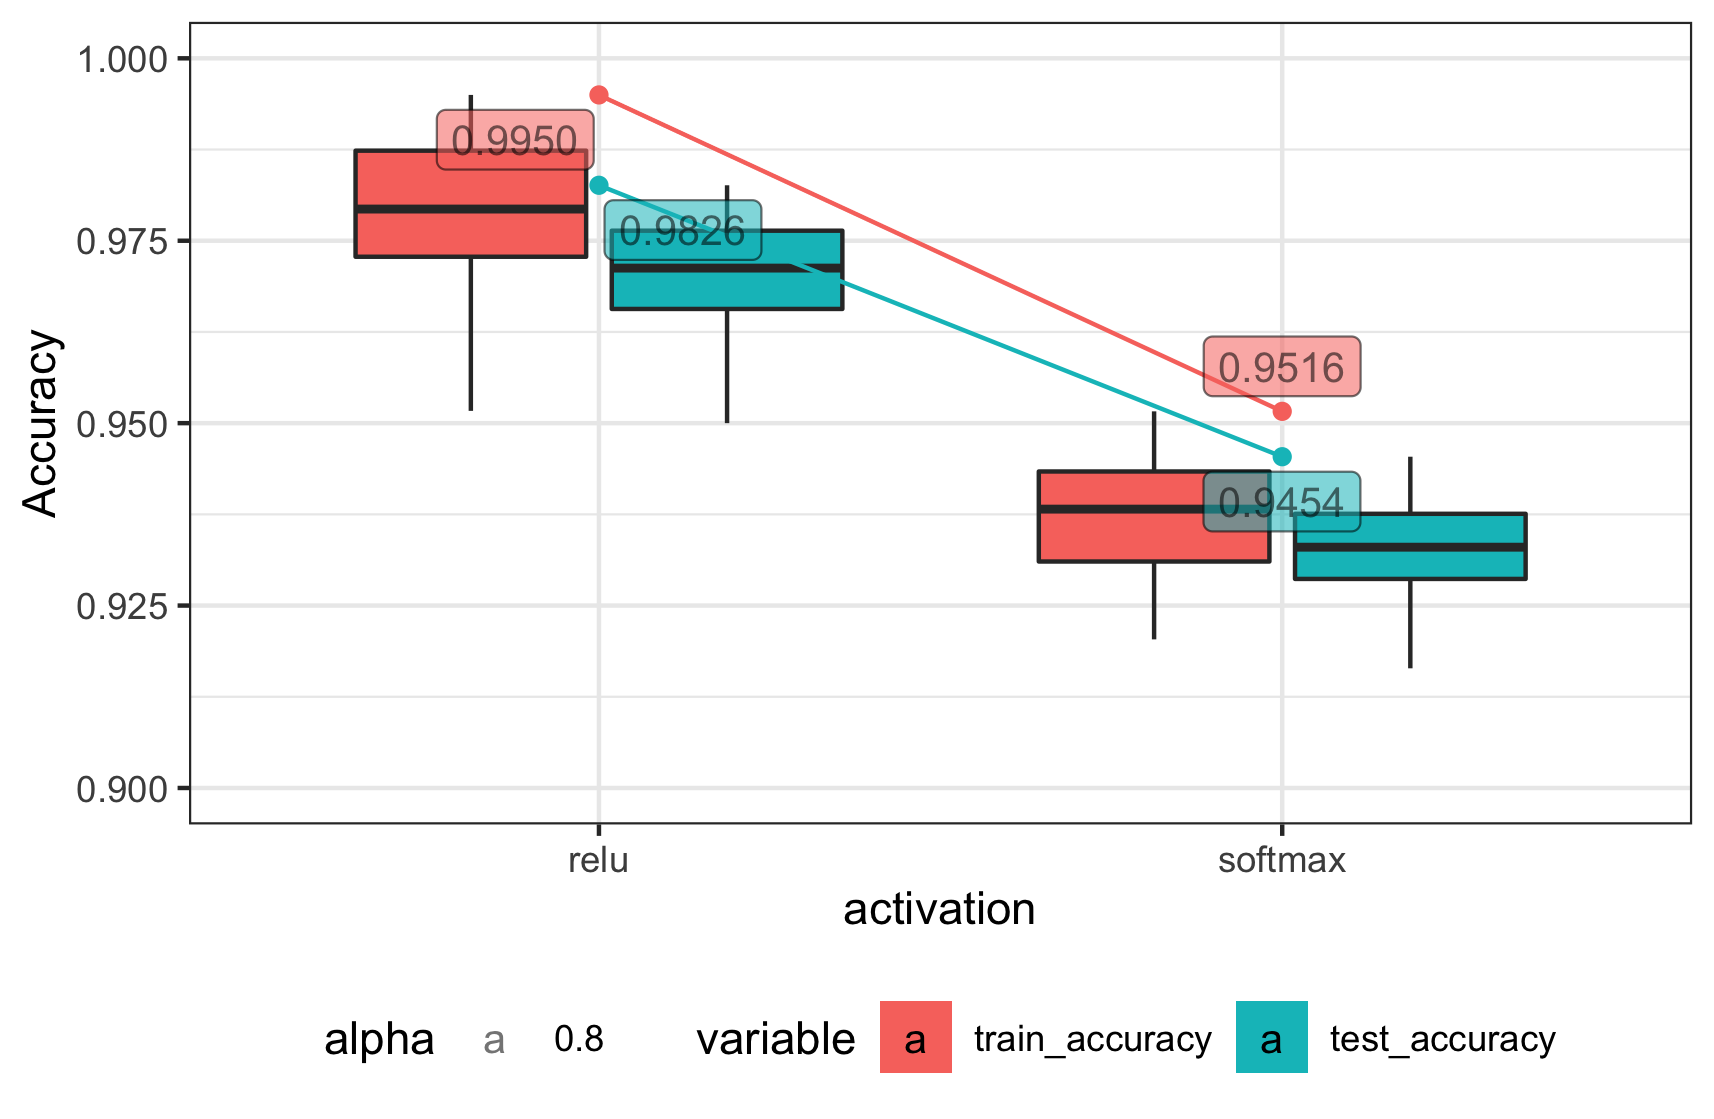
\includegraphics[width=0.8\textwidth]{figure/1-Hidden Layer Neural Network Accuracy rate versus activation.png}} 
\caption{1-Hidden Layer Neural Network Accuracy rate versus activation}
\label{1-Hidden Layer Neural Network Accuracy rate versus activation}
\vspace{-1.5em}
\end{figure}

From Fig. \ref{1-Hidden layer Neural Network Accuracy rate By Epoch}, we can see that ReLU activation greatly shortened the converge time of neural network.
\begin{figure}[htbp]
\centerline{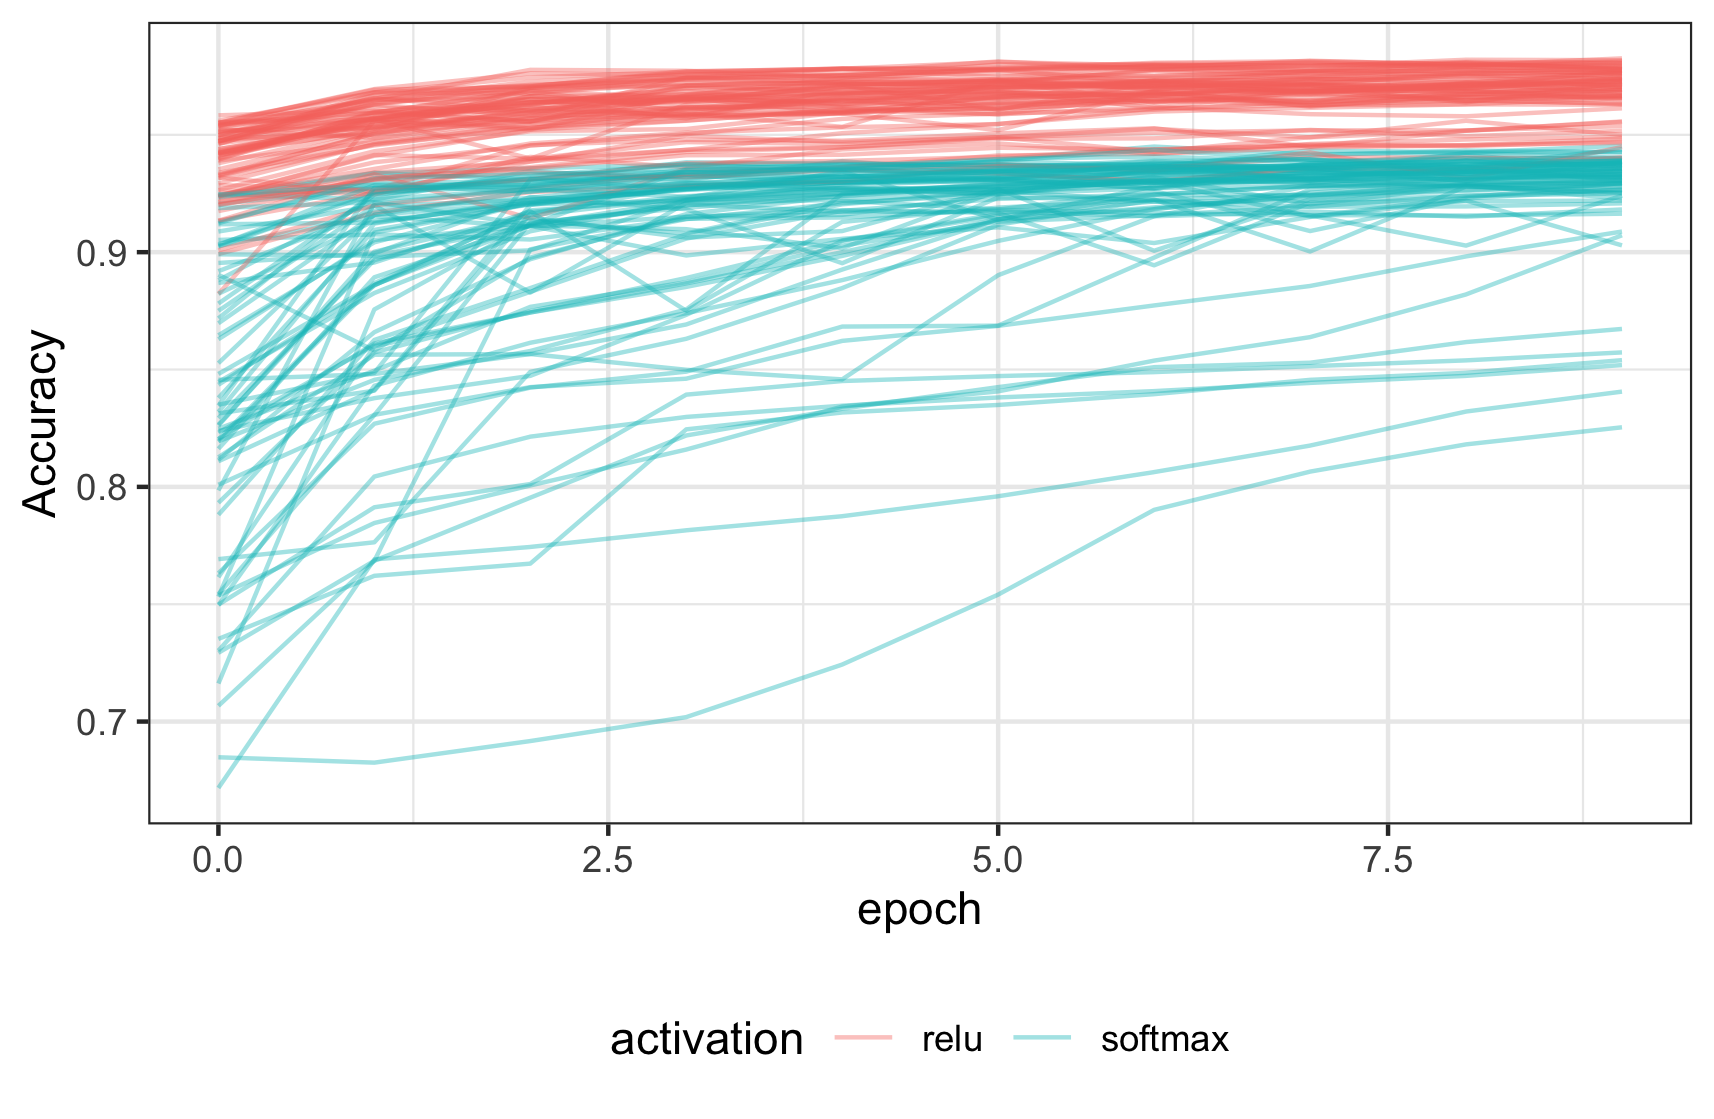
\includegraphics[width=0.8\textwidth]{figure/1-Hidden layer Neural Network Accuracy rate By Epoch.png}}
\caption{1-Hidden layer Neural Network Accuracy rate By Epoch}
\label{1-Hidden layer Neural Network Accuracy rate By Epoch}
\vspace{-1.5em}
\end{figure}
\end{frame}


















\subsection{2-layer Neutral Network}
\begin{frame}[allowframebreaks]{\secname : \subsecname}
We didn't introduce bias term in this section and skipped the learning rate of 0.1 when tunning hyper-parameters and only uses ReLU activation function. We trained 648 2-layer Neutral Network models with different hidden nodes, learning rates and bias, and for every type of model we trained 10 epochs. The hyper-parameter field are as follows:
\begin{itemize}
  \item Number of hidden nodes of 1st layer: 20, 50, 100, 150, 250, 500;
  \item Number of hidden nodes of 2nd layer: 20, 50, 100, 150, 250, 500;
  \item batch size: 100, 200, 300;
  \item loss function: mean squared error, categorical cross-entropy;
  \item Learning rate: 0.001, 0.01.
\end{itemize}

\begin{figure}[htbp]
\centerline{\includegraphics[width=0.8\textwidth]{figure/2-layer Neural Network Test Accuracy By Epoch.png}}
\caption{2-layer Neural Network Test Accuracy By Epoch(ReLU)-1}
\label{2-layer Neural Network Test Accuracy By Epoch(ReLU)-1}
\end{figure}
\begin{figure}[htbp]
\centerline{\includegraphics[width=0.8\textwidth]{figure/2-layer Neural Network Test Accuracy By Epoch2.png}}
\caption{2-layer Neural Network Test Accuracy By Epoch(ReLU)-2}
\label{2-layer Neural Network Test Accuracy By Epoch(ReLU)-2}
\end{figure}
First, we need to know if all our model is converged. From Fig. \ref{2-layer Neural Network Test Accuracy By Epoch(ReLU)-1} and Fig. \ref{2-layer Neural Network Test Accuracy By Epoch(ReLU)-2}, we can see that all of our models are converged. And from Fig. \ref{2-layer Neural Network Test Accuracy By Epoch(ReLU)-1}, we can see that with the number of 1st hidden layer nodes going up, the test accuracy going up.

Next, we tune all the hyper-parameters.
\begin{figure}[htbp]
\centerline{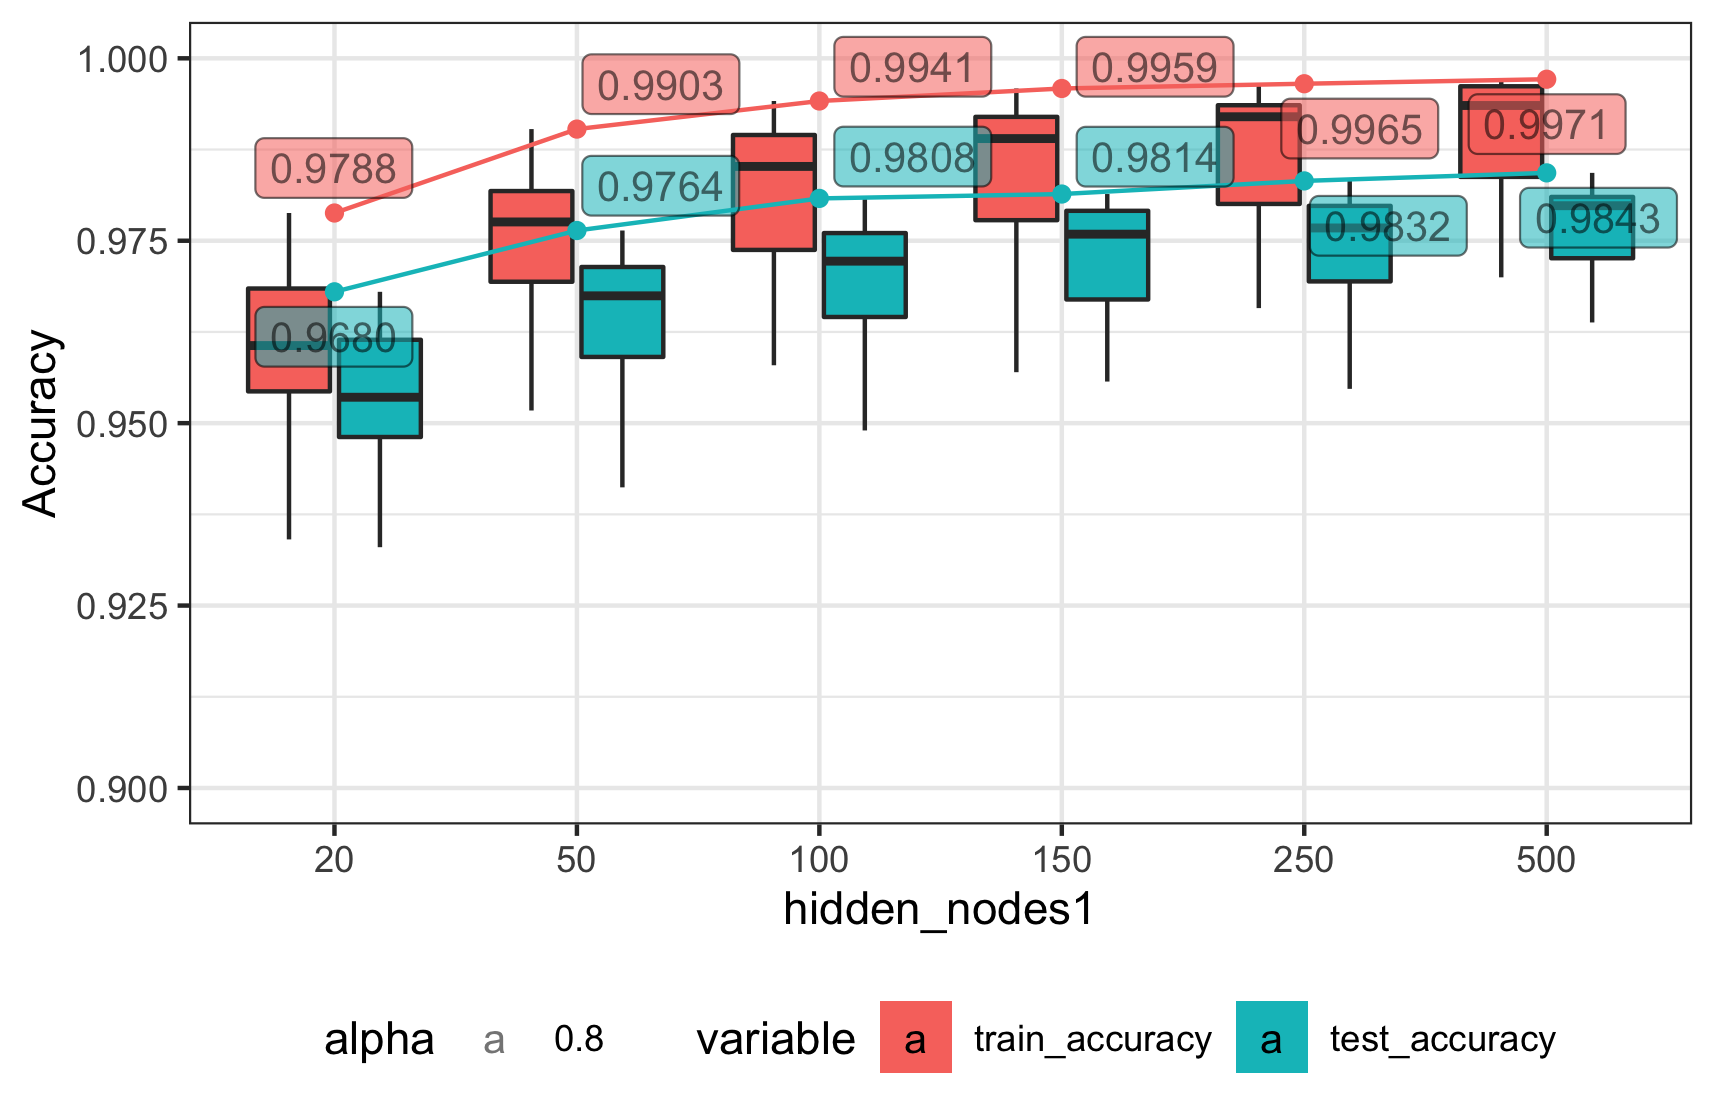
\includegraphics[width=0.8\textwidth]{figure/2-Hidden Layer Neural Network Accuracy rate versus hidden_nodes1.png}}
\caption{2-Hidden Layer NN Accuracy rate versus hidden nodes of 1st layer(ReLU)}
\label{2-Hidden Layer Neural Network Accuracy rate versus hidden nodes of 1st layer(ReLU)}
\vspace{-1.5em}
\end{figure}
From Fig. \ref{2-Hidden Layer Neural Network Accuracy rate versus hidden nodes of 1st layer(ReLU)} and Fig. \ref{2-Hidden Layer Neural Network Accuracy rate versus hidden nodes of 2nd layer(ReLU)}, we can see that the more 1st layer hidden nodes, the better the maximum test accuracy is, the more 2nd layer hidden nodes, the larger the variance of test accuracy is.
\begin{figure}[htbp]
\centerline{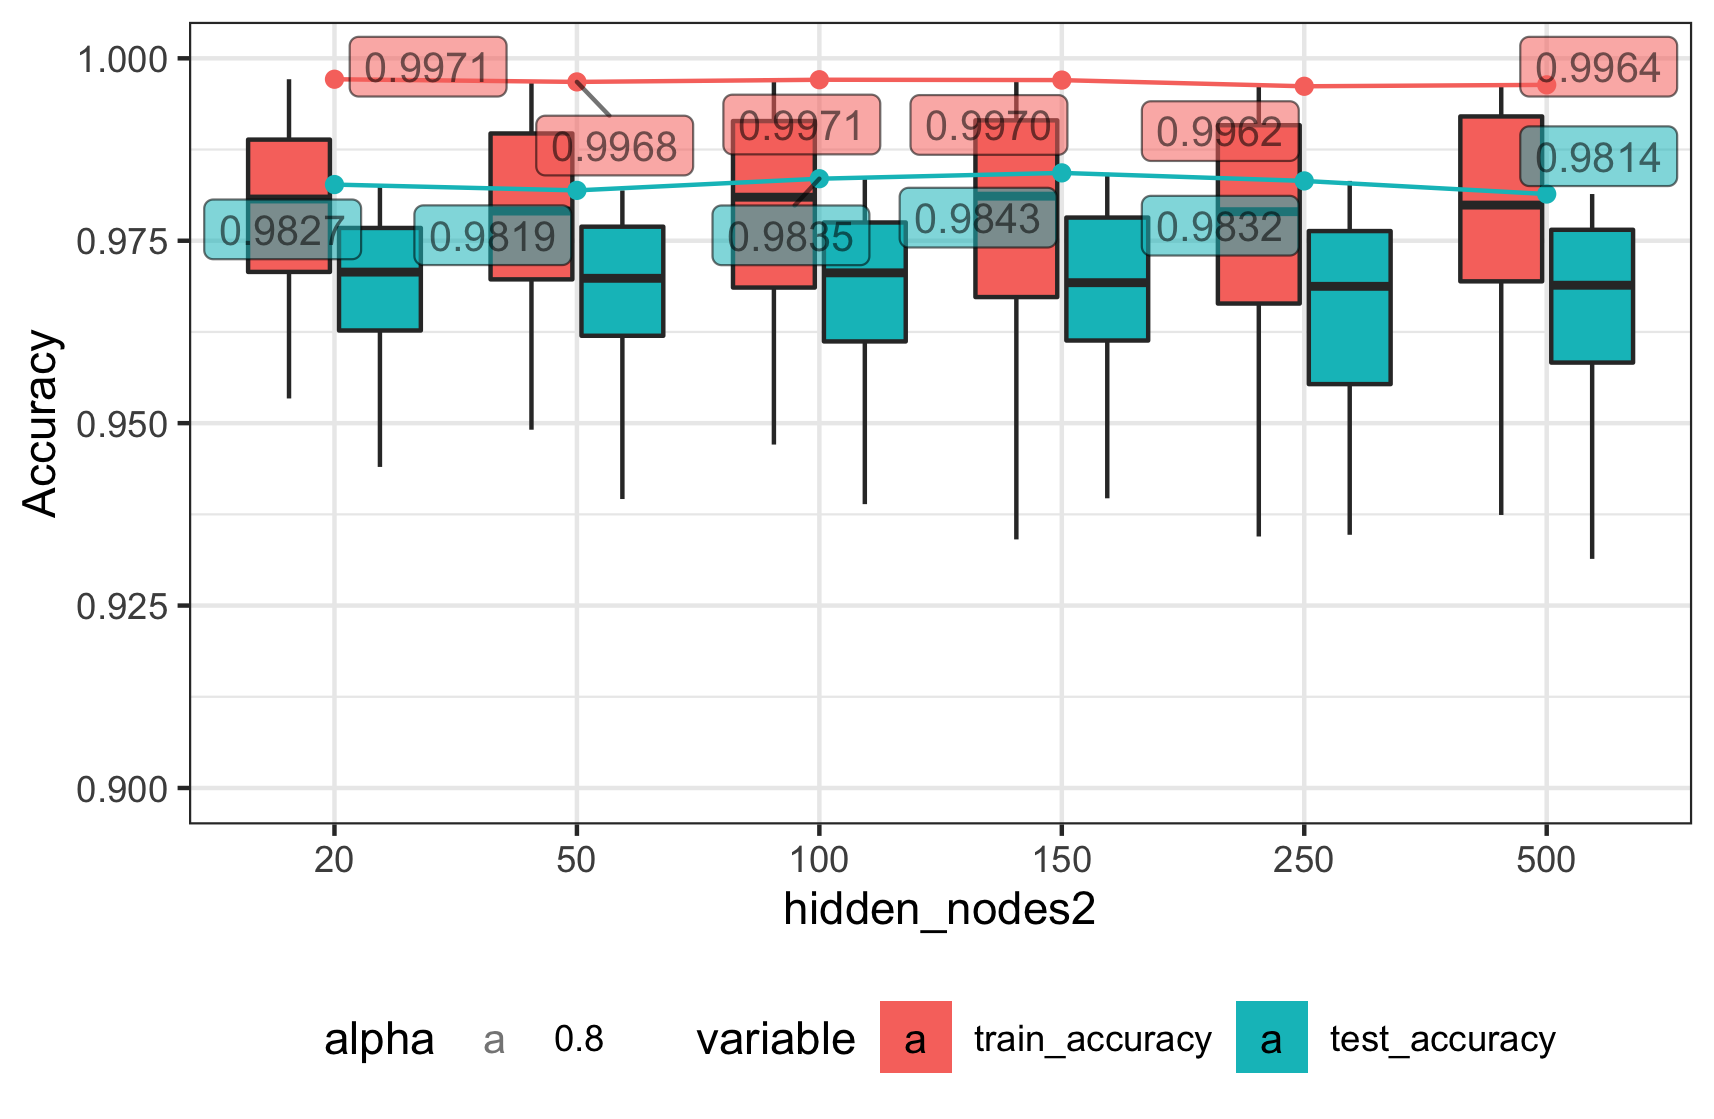
\includegraphics[width=0.8\textwidth]{figure/2-Hidden Layer Neural Network Accuracy rate versus hidden_nodes2.png}}
\caption{2-Hidden Layer NN Accuracy rate versus hidden nodes of 2nd layer(ReLU)}
\label{2-Hidden Layer Neural Network Accuracy rate versus hidden nodes of 2nd layer(ReLU)}
\end{figure}

From Fig. \ref{2-Hidden Layer Neural Network Accuracy rate versus learning rate(ReLU)}, we can see that a learning rate of 0.001 is better than 0.01.
\begin{figure}[htbp]
\centerline{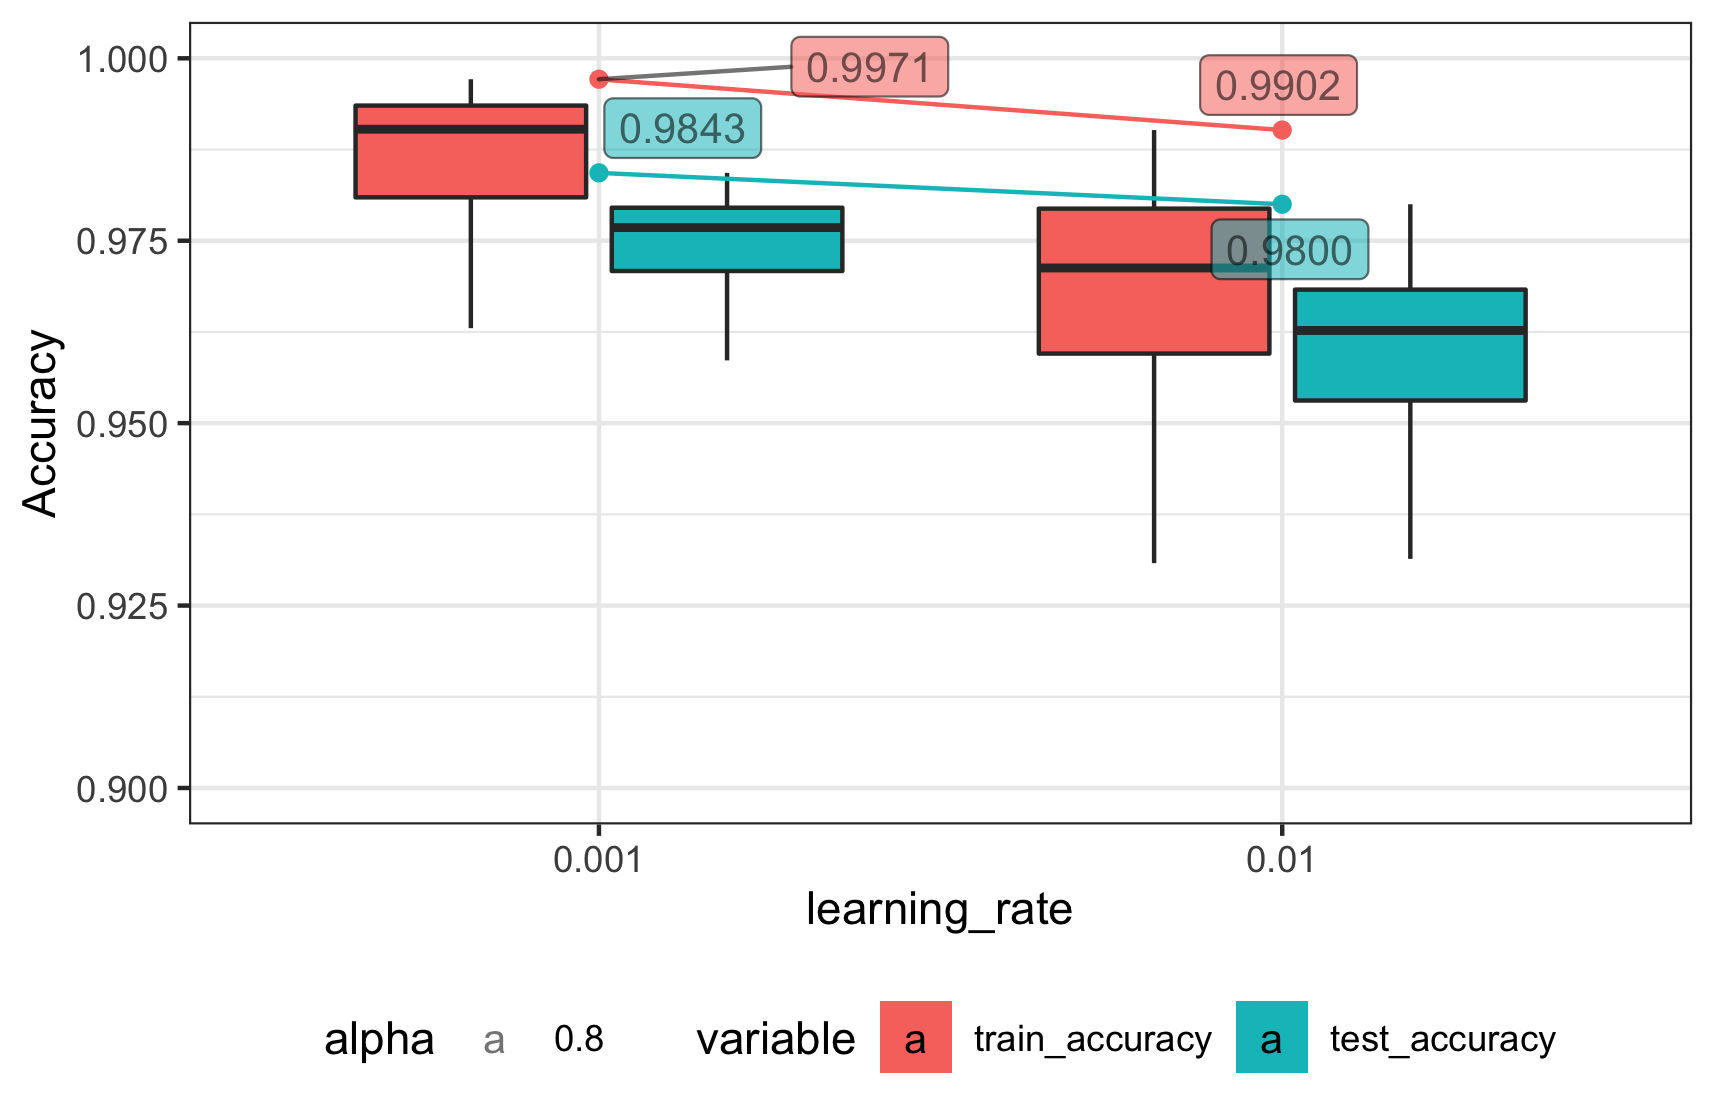
\includegraphics[width=0.8\textwidth]{figure/2-Hidden Layer Neural Network Accuracy rate versus learning_rate.png}}
\caption{2-Hidden Layer Neural Network Accuracy rate versus learning rate(ReLU)}
\label{2-Hidden Layer Neural Network Accuracy rate versus learning rate(ReLU)}
\end{figure}

From Fig. \ref{2-Hidden Layer Neural Network Accuracy rate versus loss(ReLU)}, we conclude loss function barely impact accuracy.
\begin{figure}[htbp]
\centerline{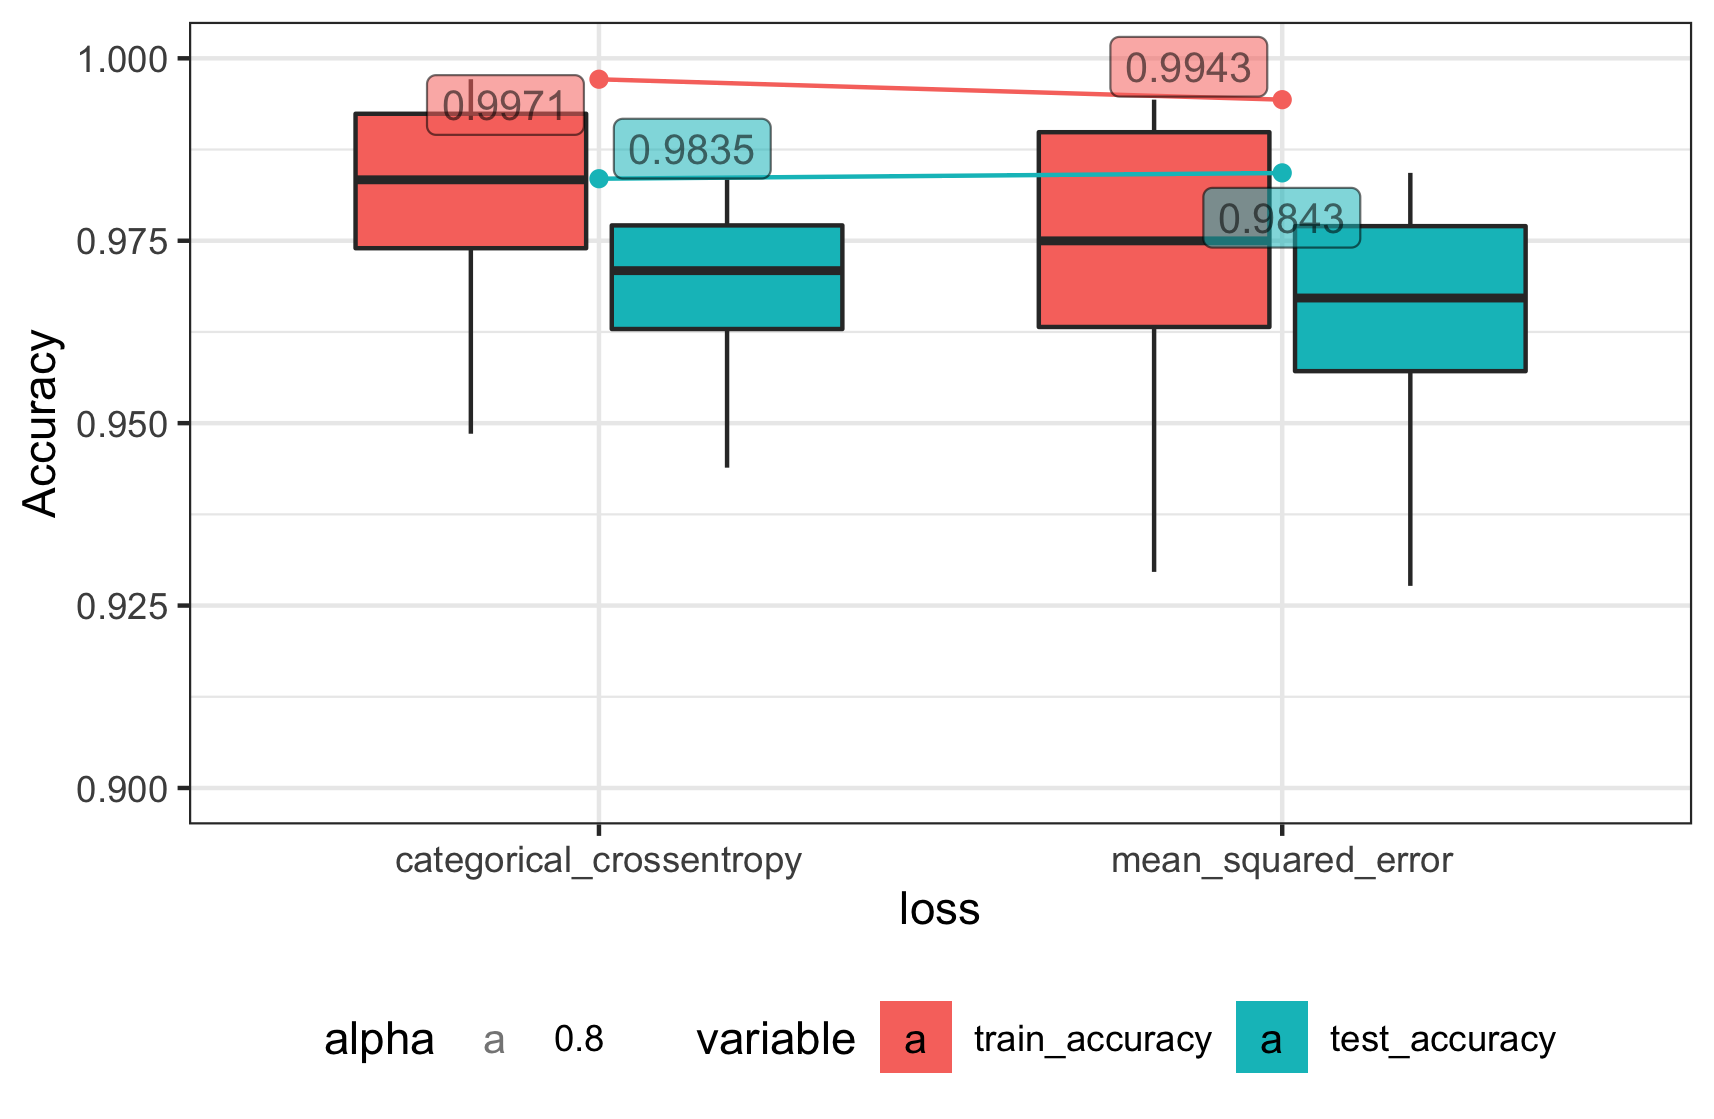
\includegraphics[width=0.8\textwidth]{figure/2-Hidden Layer Neural Network Accuracy rate versus loss.png}}
\caption{2-Hidden Layer NN Accuracy rate versus loss(ReLU)}
\label{2-Hidden Layer Neural Network Accuracy rate versus loss(ReLU)}
\end{figure}

From Fig. \ref{2-Hidden Layer Neural Network Accuracy rate versus batch size(ReLU)}, we conclude batch size barely impact accuracy.
\begin{figure}[htbp]
\centerline{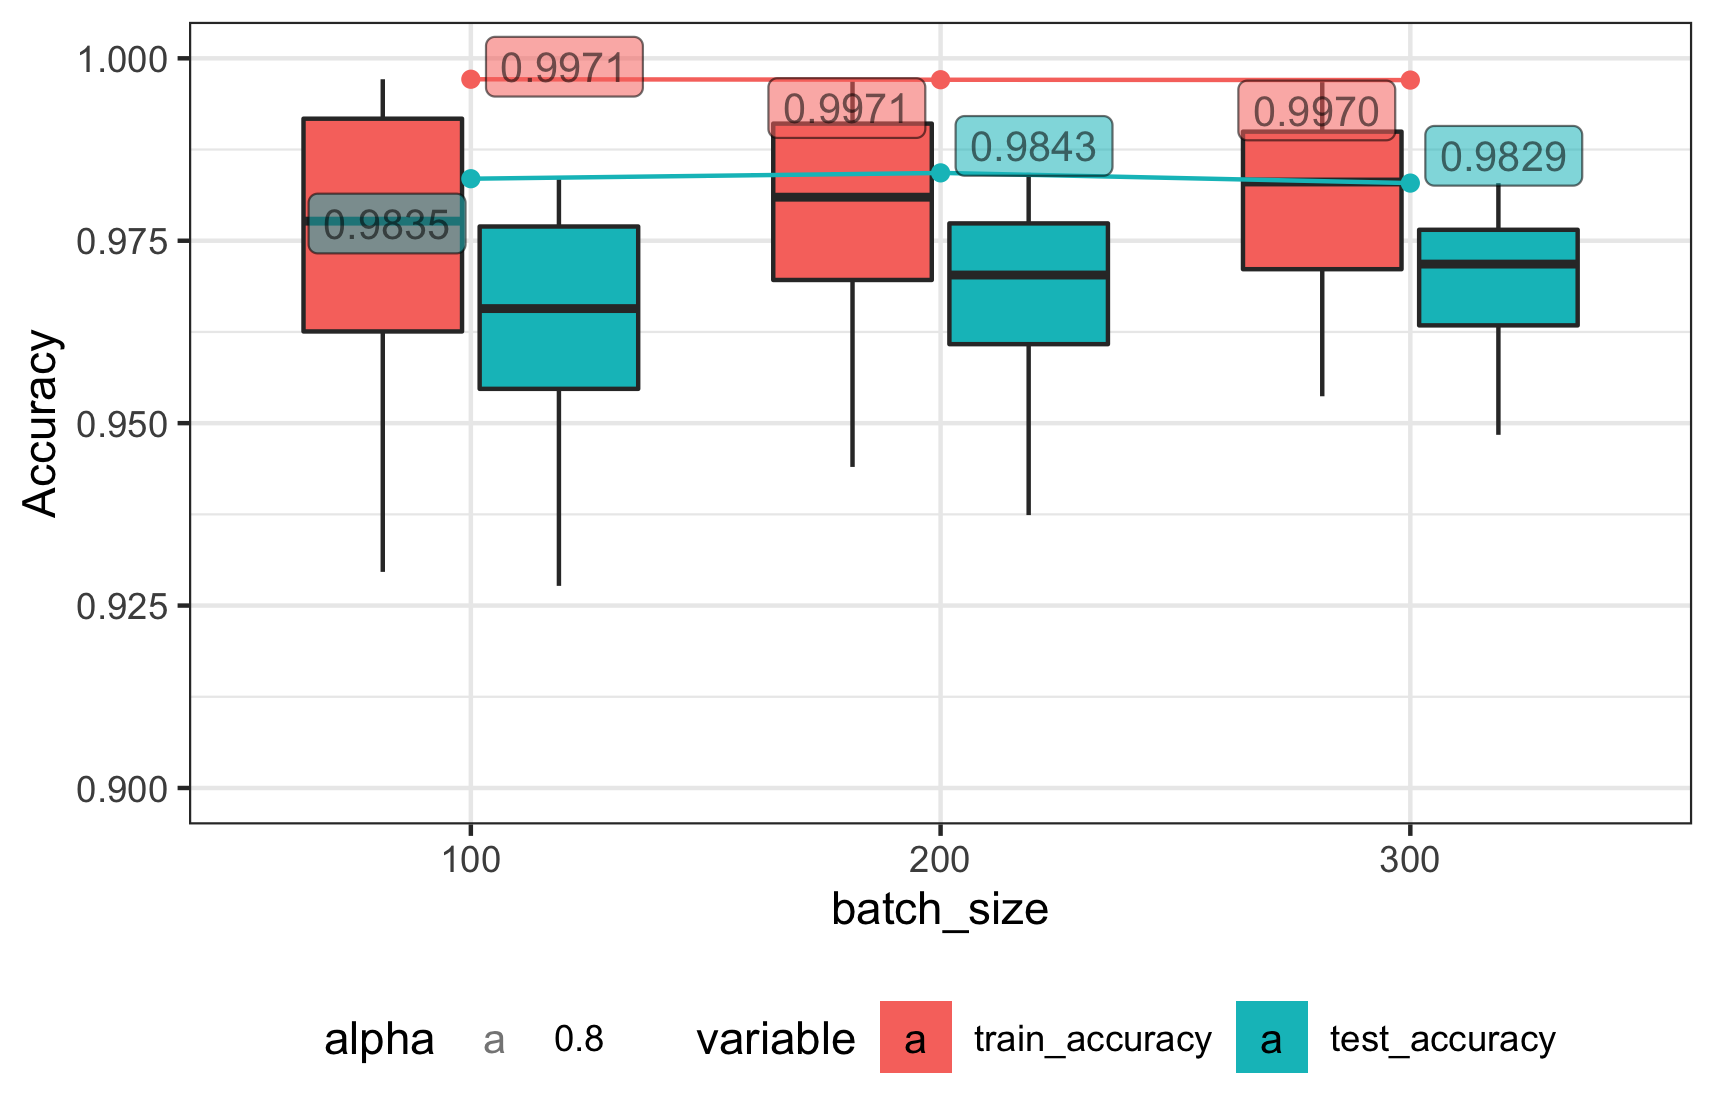
\includegraphics[width=0.8\textwidth]{figure/2-Hidden Layer Neural Network Accuracy rate versus batch_size.png}}
\caption{2-Hidden Layer NN Accuracy rate versus batch size(ReLU)}
\label{2-Hidden Layer Neural Network Accuracy rate versus batch size(ReLU)}
\vspace{-1.5em}
\end{figure}




\begin{itemize}
  \item The hyper-parameter of best model is as TABLE \ref{2-layer Neutral Network best hyper-parameter(ReLU)}
  \item The test accuracy is 0.9843, train accuracy is 0.9971, and the confusion table is as TABLE \ref{2-layer Neutral Network confusion table}. 
  \item Here, we achieved a slight improvement than the 1 hidden layer neural network.
\end{itemize}

\begin{table}[htbp]
\tiny
\centering
\caption{2-layer Neutral Network best hyper-parameter(ReLU)}
\begin{tabular}{|c|c|c|c|}
  \hline
 hidden\_nodes1& hidden\_nodes2 & activation & batch\_size  \\

500& 150& ReLU & 200  \\
  \hline
learning\_rate & epoch & variable & value \\ 

 0.001 &   10 & test\_accuracy & 0.9843 \\ 
    \hline
 loss&&&\\
 mean\_squared\_error&&&\\
   \hline
\end{tabular}
\label{2-layer Neutral Network best hyper-parameter(ReLU)}	
\end{table}
% Table generated by Excel2LaTeX from sheet 'Sheet1'
\begin{table}[htbp]
\tiny
  \centering
  \caption{2-layer Neutral Network confusion table}
% Table generated by Excel2LaTeX from sheet 'Sheet2'
\begin{tabular}{|r|rrrrrrrrrr|r|}
\hline
  & 0 & 1 & 2 & 3 & 4 & 5 & 6 & 7 & 8 & 9 &  \\
\hline
  & 0 & 1 & 2 & 3 & 4 & 5 & 6 & 7 & 8 & 9 &  \\
0 & 975 & 1 & 0 & 0 & 1 & 1 & 1 & 1 & 1 & 0 & 0.9939 \\
1 & 0 & 1129 & 1 & 2 & 0 & 1 & 2 & 0 & 0 & 0 & 0.9947 \\
2 & 4 & 3 & 1002 & 3 & 5 & 0 & 4 & 6 & 4 & 0 & 0.9719 \\
3 & 0 & 1 & 1 & 1000 & 0 & 4 & 0 & 4 & 4 & 1 & 0.9852 \\
4 & 0 & 2 & 3 & 0 & 968 & 0 & 2 & 0 & 0 & 7 & 0.9857 \\
5 & 3 & 1 & 0 & 5 & 1 & 867 & 7 & 0 & 2 & 1 & 0.9775 \\
6 & 2 & 2 & 0 & 1 & 8 & 4 & 941 & 0 & 0 & 0 & 0.9823 \\
7 & 1 & 5 & 4 & 2 & 0 & 0 & 0 & 1007 & 4 & 5 & 0.9796 \\
8 & 2 & 1 & 2 & 3 & 3 & 1 & 4 & 3 & 953 & 2 & 0.9784 \\
9 & 3 & 4 & 0 & 4 & 8 & 9 & 1 & 4 & 4 & 972 & 0.9633 \\
\hline
  & 0.9848 & 0.9826 & 0.9891 & 0.9804 & 0.9738 & 0.9775 & 0.9782 & 0.9824 & 0.9805 & 0.9838 & 0.9843 \\
\hline
\end{tabular}%
  \label{2-layer Neutral Network confusion table}%
\end{table}%

\end{frame}










\section{Conclusion}
\begin{frame}[allowframebreaks]{\secname}
\begin{table}[htbp]
  \centering
  \caption{Comparison}
    \begin{tabular}{lccc}
\hline
    Method & \multicolumn{1}{l}{Train Accurancy} & \multicolumn{1}{l}{Test Accurancy} & \multicolumn{1}{l}{Time(Second)} \\
\hline
    SVM Linear Kernel & 0.9239 & 0.9178 & 344 \\
    SVM RBF Kernel & 0.9983 & 0.9852 & 2,749 \\
    SVM Polynomial Kernel & 0.9989 & 0.9806 & 1,439 \\
% Table generated by Excel2LaTeX from sheet 'Sheet3'
	Gradient Boosting & 0.9981 & 0.9673 & 7,321 \\
	Ada Boosting & 0.8911 & 0.8902 & 1,402 \\
    \makecell[l]{1-layer NN 150\\\quad (Softmax)}  & 0.9516 & 0.9454 & 30 \\
    \makecell[l]{1-layer NN 500\\\quad(ReLU)}  & 0.9950 & 0.9826 & 40 \\
    \makecell[l]{2-Layer NN 500-150\\\quad(ReLU,ReLU)} & 0.9971 & 0.9843 & 57 \\
\hline
    \end{tabular}%
  \label{tab:Comparison}%
\end{table}%
\begin{itemize}
  \item From TABLE \ref{tab:Comparison}, we can see that SVM with RBF kernel have the best test accuracy, but it takes a lot of time to train. 
  \item The second best model is 2-layer neural network with 500-150 hidden nodes and ReLU activation function, and it only takes 57 seconds to train the model. 
  \item The test accuracy difference of these 2 model is only 0.0008, but the time difference is nearly 3,000 seconds. 
  \item Therefore, we conclude that for MNIST data, the best model, considering test accuracy and training time, is 2-layer neural network with 500-150 hidden nodes and ReLU activation function.
\end{itemize}

\end{frame}








%\section{Futrue works}
%\begin{frame}[allowframebreaks]{\secname}
%\begin{enumerate}
%  \item Try more nodes on 2-Layer Neural Network
%  \item Try some tree based method
%  \item Try KNN
%  \item Try tune SVM with global optimazation
%\end{enumerate}	
%\end{frame}





%\subsubsection{Convolutional net LeNet-4}
%When we start learning deep learning with neural network, we realize that one of the most powerful supervised deep learning techniques is the Convolutional Neural Networks (abbreviated as “CNN”).


%\section{Conclusion}
%


%\section{Futrue works}
%\begin{frame}{\secname}
%\begin{itemize}
%  \item More method	
%  \begin{itemize}
%	  \item Tree method
%	  \begin{itemize}
%	  \item Random forest
%	  \item Boosting
%	  \end{itemize}
%	
%	  \item SVM with different kernel
%	  \begin{itemize}
%	  \item RBF kernel
%	  \item Polynomial kernel.
%	  \end{itemize}
%	
%	  \item Convolutional Neural Network
%  \end{itemize}
%  \item Running time comparison.
%\end{itemize}
%
%
%\end{frame}


\section{References}
\begin{frame}[label=bibliography,allowframebreaks]{\secname}
\scriptsize
  \bibliographystyle{unsrt}
  \bibliography{references}
\end{frame}


\section{Questions}
\begin{frame}[allowframebreaks]{\secname}
\begin{itemize}
  \item Questions?
\end{itemize}
\end{frame}



\end{document}